\chapter{Вычисления} \label{chapter:computations}

В данной главе рассматриваются вопросы выполнения вычислений применительно к задаче нахождения одного или нескольких решений однородной системы:

$$
	S X = 0,
$$

где $S$ --- несимметричная матрица, ранг которой меньше количества столбцов в матрице $S$.

Для применения метода Ланцоша--Монтгомери матрица системы симметризуется путем умножения слева на матрицу $S^T$:

$$
	S^T S X = 0.
$$

\section{Схема вычисления} \label{section:computational_scheme}

В соответствии с методом решения однородной системы уравнений прежде всего необходимо сформировать случайным образом матрицу $Y$ порядка $n \times n_b$ и вычислить
матрицу $S^T S Y$:

\computationstep{сформировать случайным образом $Y$}
\computationstep{вычислить матрицу $B = S^T S Y$}

Полученная матрица $B$ принимается в качестве правой части неоднородной системы \ref{equation:ti:nhs:non_homogeneous_equation_system},
для которой необходимо найти решение по методу Ланцоша--Монтгомери, изложенному в разделе \ref{section:ti:non_homogeneous_systems}.

Согласно методу столбцы матрицы $B$ используются в качестве начального набора столбцов $V_1$.

\computationstep{$V_1 = B$}

Далее начинается итерационная часть алгоритма, в которой номер $i$ используется как номер подпространства:

\computationstep{$i = 1$}

В начале каждой итерации необходимо из столбцов матрицы $V_i$ сформировать матрицу $W_i$ такую, что:

\begin{enumerate}
	\item матрица $Q_i = W_i^T S^T S W_i$ является невырожденной;
	\item матрица $W_i$ содержит наибольшее возможное количество столбцов,
\end{enumerate}

а затем еще вычислить обратную матрицу $Q_i^{-1}$.

Определение столбцов $W_i$ и нахождение матрицы $Q_i^{-1}$, вообще говоря, можно выполнять схожими способами на основе метода исключения Гаусса, поэтому существуют
такие алгоритмы, которые одновременное решают обе задачи. Один из таких алгоритмов приводит в своей статье \cite{Montgomery} Монтгомери.

Прежде всего необходимо вычислить матрицу $S W_i$. К сожалению, на этом этапе пока еще не известно какие столбцы из $V_i$ образуют $W_i$, поэтому приходится вычислять
матрицу $S V_i$, которая содержит $S W_i$ как подматрицу:

\computationstep{вычислить $V_i^{(S)} = S V_i$}

Используя полученную матрицу $V_i^{(S)}$, необходимо вычислить расширенную матрицу $\widetilde{Q}_i$, которая включает в себя матрицу $Q_i$ как подматрицу:

\computationstep{вычислить $\widetilde{Q}_i = {\left ( V_i^{(S)} \right )}^T V_i^{(S)} \left ( = {\left ( S V_i \right )}^T \left ( S V_i \right ) \right ) $}

Вообще говоря, расширенная матрица $\widetilde{Q}_i$ может оказаться вырожденной, тем не менее если расширенная матрица $\widetilde{Q}_i$ ненулевая, то в ней можно
выделить невырожденную подматрицу $Q_i$. Причем поскольку матрица $\widetilde{Q}_i$ является симметричной, то можно сделать так, чтобы набор строк и набор столбцов,
на пересечении которых размещаются элементы подматрица $Q_i$, совпадали. Кроме того, крайне желательно, чтобы невырожденная подматрица $Q_i$ содержала бы как можно
больше строк/столбцов, поскольку набор номеров столбцов, из которых составлена подматрица $Q_i$, является тем самым набором номеров столбцов матрицы $V_i$, которые
выбираются для формирования матрицы $W_i$. Далее для выделенной подматрицы $Q_i$ необходимо найти обратную к ней матрицу $Q_i^{-1}$.

Упомянутый ранее алгоритм Монтгомери (из статьи \cite{Montgomery}) позволяет найти обратную матрицу $Q_i^{-1}$, точнее алгоритм Монтгомери формирует расширенную
матрицу $\widetilde{Q}_i^{(inv)}$ и набор номеров столбцов (он же набор номеров строк), на пересечении которых размещаются элементы матрицы $Q_i^{-1}$.

\computationstep{по алгоритму Монтгомери вычислить $\widetilde{Q}_i^{(inv)}$, одновременно определив набор столбцов матрицы $V_i$, которые войдут в состав $W_i$}

После вычисления $\widetilde{Q}_i^{(inv)}$ появляется возможность "выделения"{} обратной матрицы $Q_i^{-1}$, которую необходимо умножить справа на $W_i$:

\computationstep{вычислить $W_i^{(Q)} = W_i Q_i^{-1} \left ( = W_i {\left ( W_i^T S^T S W_i \right ) }^{-1} \right )$}

Вычисленную матрицу $W_i^{(Q)}$ нужно сохранить, поскольку она используется в трех дальнейших $S^TS$-ортогонализациях.

Далее остается лишь вычислить произведение $W_i^T B$:

\computationstep{вычислить $W_i^{(B)} = W_i^T B$}

\noindent и модифицировать текущее "приближение"{} к решению:

\computationstep{вычислить $X = X + W_i^{(Q)}W_i^{(B)}$}

После модификации "приближения"{} $X$ необходимо перейти к вычислению следующего набора векторов $V_{i+1}$.

При вычислении $\widehat{V}_{i+1}$ можно использовать два шага: во-первых, вычислить $S^T V_i^{(S)}$ (это будет матрица
$[ \begin{array}{cc} S^T S \widehat{W}_i & B^T B \widehat{W}_i \end{array}]$):

\computationstep{вычислить $\widehat{V}_{i+1} = S^T V_i^{(S)}$}

во-вторых, в столбцах $S^T \widehat{W_i}$), вернуть столбцы $\widehat{W}_i$ из матрицы $V_i$, в результате получится матрица
$[ \begin{array}{cc} \widehat{W}_i & S^T S \widehat{W}_i \end{array}]$

\computationstep{в матрице $\widehat{V}_{i+1}$ вернуть столбцы $\widehat{W}_i$, взяв их из матрицы $V_i$}

Теперь необходимо $S^T S$-ортогонализовать полученный набор столбцов $\widehat{V}_{i+1}$ путем вычисления соотношения:

$$
	\begin{array}{ccl}
		V_{i+1} & = & \widehat{V}_{i+1} + \\
	        &   & + W_{(i+1)-1} \left ( W_{(i+1)-1}^T S^T S W_{(i+1)-1} \right ) ^{-1} W_{(i+1)-1}^T S^T S \widehat{V}_{i+1} + \\
	        &   & + W_{(i+1)-2} \left ( W_{(i+1)-2}^T S^T S W_{(i+1)-2} \right ) ^{-1} W_{(i+1)-2}^T S^T S \widehat{V}_{i+1} + \\
	        &   & + W_{(i+1)-3} \left ( W_{(i+1)-3}^T S^T S W_{(i+1)-3} \right ) ^{-1} W_{(i+1)-3}^T S^T S \widehat{V}_{i+1}
	\end{array}
	,
$$

в котором некоторые матрицы уже вычислены, в частности:

$$
	\begin{array}{lll}
		W_i^{(Q)}     & = & W_{(i+1)-1} \left ( W_{(i+1)-1}^T S^T S W_{(i+1)-1} \right ) ^{-1} \\
		W_{i-1}^{(Q)} & = & W_{(i+1)-2} \left ( W_{(i+1)-2}^T S^T S W_{(i+1)-2} \right ) ^{-1} \\
		W_{i-2}^{(Q)} & = & W_{(i+1)-3} \left ( W_{(i+1)-3}^T S^T S W_{(i+1)-3} \right ) ^{-1} .
	\end{array}
$$

Таким образом,

$$
	\begin{array}{ccl}
		V_{i+1} & = & \widehat{V}_{i+1} + \\
	        &   & + W_i^{(Q)}     W_{i}^T   S^T S \widehat{V}_{i+1} + \\
	        &   & + W_{i-1}^{(Q)} W_{i-1}^T S^T S \widehat{V}_{i+1} + \\
	        &   & + W_{i-2}^{(Q)} W_{i-2}^T S^T S \widehat{V}_{i+1} .
	\end{array}
$$

Далее, матрица $W_{i}^T S^T S$ является подматрицей матрицы $\widehat{V}_{i+1}^T$, точно так же как $W_{i-1}^T S^T S$ является подматрицей $\widehat{V}_{i+1}^T$,
а $W_{i-2}^T S^T S$ --- $\widehat{V}_{i-1}^T$, поэтому их можно представить в виде:

$$
	\begin{array}{ccl}
		W_{i}^T S^T S   & = & J_{i-1} \widehat{V}_{i+1}^T \\
		W_{i-1}^T S^T S & = & J_{i-2} \widehat{V}_{i}^T \\
		W_{i-2}^T S^T S & = & J_{i-3} \widehat{V}_{i-1}^T ,
	\end{array}
$$

где матрицы $J_{i-1}$, $J_{i-2}$ и $J_{i-3}$ --- проецирующие матрицы, выделяющие строки, соответствующие $W_{i}^T S^T S$, $W_{i-1}^T S^T S$ и $W_{i-2}^T S^T S$,
и отбрасывающие остальные (ненужные) строки.

Таким образом, выполнение $S^T S$-ортогонализации в конечном счете имеет вид:

$$
	\begin{array}{ccl}
		V_{i+1} & = & \widehat{V}_{i+1} + \\
	        &   & + W_i^{(Q)}     J_{i-1} \widehat{V}_{i+1}^T \widehat{V}_{i+1} + \\
	        &   & + W_{i-1}^{(Q)} J_{i-2} \widehat{V}_{i}^T   \widehat{V}_{i+1} + \\
	        &   & + W_{i-2}^T     J_{i-3} \widehat{V}_{i-1}^T \widehat{V}_{i+1} .
	\end{array}
$$

\begin{figure}
	\begin{tikzpicture}[scale=16]
		\node [above] at ( 0.00, 0.00 ) {$Y$};
		\draw [->] ( 0.00, 0.00 ) -- ( 0.00, -0.06 );
		\node [above] at ( 0.00, -0.10 ) {$S Y$};
		\draw [->] ( 0.00, -0.10 ) -- ( 0.00, -0.16 );
		\node [above] at ( 0.00, -0.20 ) {$B = S^T S Y$};
	\end{tikzpicture}
	\caption{Переход к решению неоднородной системы}
\end{figure}

\begin{figure}
	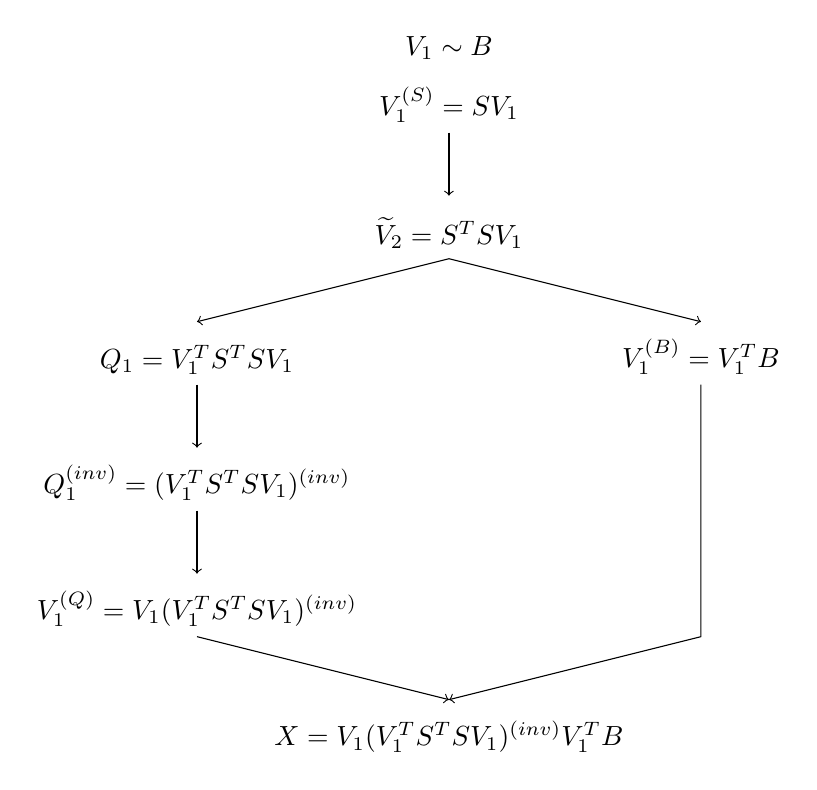
\begin{tikzpicture}[scale=16]
		\node [above] at ( 0.00, 0.05 ) {$V_1 \sim B$};
		\node [above] at ( 0.00, 0.00 ) {$V_1^{(S)} = S V_1$};
		\draw [->] ( 0.00, 0.00 ) -- ( 0.00, -0.05 );
		\node [above] at ( 0.00, -0.10 ) {$\widetilde{V}_{2} = S^T S V_1$};
		\draw [->] ( 0.00, -0.10 ) -- ( -0.20, -0.15 );
		\draw [->] ( 0.00, -0.10 ) -- ( 0.20, -0.15 );
		\node [above] at ( -0.20, -0.20 ) {$Q_1 = V_1^T S^T S V_1$};
		\draw [->] ( -0.20, -0.20 ) -- ( -0.20, -0.25 );
		\node [above] at ( -0.20, -0.30 ) {$Q_1^{(inv)} = ( V_1^T S^T S V_1 ) ^{(inv)}$};
		\draw [->] ( -0.20, -0.30 ) -- ( -0.20, -0.35 );
		\node [above] at ( -0.20, -0.40 ) {$V_1^{(Q)} = V_1 ( V_1^T S^T S V_1 ) ^{(inv)}$};
		\draw [->] ( -0.20, -0.40 ) -- ( 0.00, -0.45 );
		\node [above] at ( 0.20, -0.20 ) {$V_1^{(B)} = V_1^T B$};
		\draw [->] ( 0.20, -0.20 ) -- ( 0.20, -0.40 ) -- ( 0.00, -0.45 );
		\node [above] at ( 0.00, -0.50 ) {$X = V_1 ( V_1^T S^T S V_1 ) ^{(inv)} V_1^T B$};
	\end{tikzpicture}
	\caption{Вычисления с первым набором направлений $V_1$}
\end{figure}

\begin{figure}
	\begin{tikzpicture}[scale=16]
		\node [above] at ( 0.00, 0.00 ) {$\widehat{V}_i = \widetilde{V}_i \leftarrow \widehat{W}_{i-1}$};
		\draw [->] ( 0.00, 0.00 ) -- ( -0.30, -0.05 );
		\draw [->] ( 0.00, 0.00 ) -- ( 0.00, -0.05 );
		\draw [->] ( 0.00, 0.00 ) -- ( 0.30, -0.05 );
		\node [above] at ( -0.35, -0.10 ) {$\widehat{V}_i^T \widehat{V}_i$};
		\node [above] at ( 0.00, -0.10 ) {$\widehat{V}_{i-1}^T \widehat{V}_i$};
		\node [above] at ( 0.35, -0.10 ) {$\widehat{V}_{i-2}^T \widehat{V}_i$};
		\draw [->] ( -0.35, -0.10 ) -- ( -0.35, -0.15 );
		\draw [->] ( 0.00, -0.10 ) -- ( 0.00, -0.15 );
		\draw [->] ( 0.35, -0.10 ) -- ( 0.35, -0.15 );
		\node [above] at ( -0.35, -0.20 ) {$V_{i-1} ( V_{i-1} S^T S V_{i-1} )^{(inv)} \widehat{V}_i^T \widehat{V}_i$};
		\node [above] at ( 0.00, -0.20 ) {$V_{i-2} ( V_{i-2} S^T S V_{i-2} )^{(inv)} \widehat{V}_{i-1}^T \widehat{V}_i$};
		\node [above] at ( 0.35, -0.20 ) {$V_{i-3} ( V_{i-3} S^T S V_{i-3} )^{(inv)} \widehat{V}_{i-2}^T \widehat{V}_i$};
		\draw [->] ( -0.35, -0.20 ) -- ( 0.00, -0.25 );
		\draw [->] ( 0.00, -0.20 ) -- ( 0.00, -0.25 );
		\draw [->] ( 0.35, -0.20 ) -- ( 0.00, -0.25 );
		\node [below] at ( 0.00, -0.25 ) {$\begin{array}{c}
												V_i = \widehat{V}_i + \\
												+ V_{i-1} ( V_{i-1} S^T S V_{i-1} )^{(inv)} \widehat{V}_i^T \widehat{V}_i + \\
												+ V_{i-2} ( V_{i-2} S^T S V_{i-2} )^{(inv)} \widehat{V}_{i-1}^T \widehat{V}_i + \\
												+ V_{i-3} ( V_{i-3} S^T S V_{i-3} )^{(inv)} \widehat{V}_{i-2}^T \widehat{V}_i
											\end{array}$};
		\draw [->] ( 0.00, -0.40 ) -- ( 0.00, -0.45 );
		\node [above] at ( 0.00, -0.50 ) {$V_i^{(S)} = S V_i$};
		\draw [->] ( 0.00, -0.50 ) -- ( 0.00, -0.55 );
		\node [above] at ( 0.00, -0.60 ) {$\widetilde{V}_{i+1} = S^T S V_i$};
		\draw [->] ( 0.00, -0.60 ) -- ( -0.20, -0.65 );
		\draw [->] ( 0.00, -0.60 ) -- ( 0.20, -0.65 );
		\node [above] at ( -0.20, -0.70 ) {$Q_i = V_i^T S^T S V_i$};
		\draw [->] ( -0.20, -0.70 ) -- ( -0.20, -0.75 );
		\node [above] at ( -0.20, -0.80 ) {$Q_i^{(inv)} = ( V_i^T S^T S V_i ) ^{(inv)}$};
		\draw [->] ( -0.20, -0.80 ) -- ( -0.20, -0.85 );
		\node [above] at ( -0.20, -0.90 ) {$V_i^{(Q)} = V_i ( V_i^T S^T S V_i ) ^{(inv)}$};
		\draw [->] ( -0.20, -0.90 ) -- ( 0.00, -0.95 );
		\node [above] at ( 0.20, -0.70 ) {$V_i^{(B)} = V_i^T B$};
		\draw [->] ( 0.20, -0.70 ) -- ( 0.20, -0.90 ) -- ( 0.00, -0.95 );
		\node [above] at ( 0.00, -1.00 ) {$X = X + V_i ( V_i^T S^T S V_i ) ^{(inv)} V_i^T B$};
	\end{tikzpicture}
	\caption{Итерационная часть: вычисления с текущим набором направлений $V_i$}
\end{figure}

\section{Схемы вычислений в многопроцессной реализации} \label{section:computational_scheme_in_multiprocess_implementation}

Для большей наглядности вычислительные схемы рассматриваются для простого частного случая сетки процессов $4 \times 3$: каждый процесс имеет свой номер строки и номер столбца,
нумерация которых начинается с 1, как и для элементов матриц.

Вычислительные схемы включают в себя 12 прямоугольников, обозначеных пунктирными линиями, каждый из которых соответствует процессу. В верхнем левом углу каждого
пунктирного прямоугольника в квадратных скобках указывается номер строки и номер столбца процесса. Эти номера указаны только на первой схеме, поскольку на всех остальных
схемах они такие же. Интересующие данные на схемах представлены прямоугольниками со сплошными линиями, причем размеры прямоугольников в некоторой мере воспроизводят размеры
матриц. Стрелки на схемах обозначают передачу данных между процессами. 

\subsection{Распределение блочных векторов}

Блочные векторы $V_i$ делятся на блоки в соответствии с сеткой процессов: 4 строки и 3 столбца.

$$
	V_i
	=
	\begin{pmatrix}
		V_{i,(1,1)} & V_{i,(1,2)} & V_{i,(1,3)} \\
		V_{i,(2,1)} & V_{i,(2,2)} & V_{i,(2,3)} \\
		V_{i,(3,1)} & V_{i,(3,2)} & V_{i,(3,3)} \\
		V_{i,(4,1)} & V_{i,(4,2)} & V_{i,(4,3)}
	\end{pmatrix}
	.
$$

Процесс с номером $[r,c]$ располагает блоком $V_{i,(r,c)}$ (рисунок \ref{figure:csmi:V_distribution}).

\begin{figure}
	\begin{tikzpicture}[scale=16]
		% решетка процессов
		\draw [dotted] ( 0.00, 0.00 ) rectangle ( 0.32, 0.24 ) node [below right] at ( 0.00, 0.24 ) {[4,1]};
		\draw [dotted] ( 0.34, 0.00 ) rectangle ( 0.66, 0.24 ) node [below right] at ( 0.34, 0.24 ) {[4,2]};
		\draw [dotted] ( 0.68, 0.00 ) rectangle ( 1.00, 0.24 ) node [below right] at ( 0.68, 0.24 ) {[4,3]};
		\draw [dotted] ( 0.00, 0.26 ) rectangle ( 0.32, 0.50 ) node [below right] at ( 0.00, 0.50 ) {[3,1]};
		\draw [dotted] ( 0.34, 0.26 ) rectangle ( 0.66, 0.50 ) node [below right] at ( 0.34, 0.50 ) {[3,2]};
		\draw [dotted] ( 0.68, 0.26 ) rectangle ( 1.00, 0.50 ) node [below right] at ( 0.68, 0.50 ) {[3,3]};
		\draw [dotted] ( 0.00, 0.52 ) rectangle ( 0.32, 0.76 ) node [below right] at ( 0.00, 0.76 ) {[2,1]};
		\draw [dotted] ( 0.34, 0.52 ) rectangle ( 0.66, 0.76 ) node [below right] at ( 0.34, 0.76 ) {[2,2]};
		\draw [dotted] ( 0.68, 0.52 ) rectangle ( 1.00, 0.76 ) node [below right] at ( 0.68, 0.76 ) {[2,3]};
		\draw [dotted] ( 0.00, 0.78 ) rectangle ( 0.32, 1.02 ) node [below right] at ( 0.00, 1.02 ) {[1,1]};
		\draw [dotted] ( 0.34, 0.78 ) rectangle ( 0.66, 1.02 ) node [below right] at ( 0.34, 1.02 ) {[1,2]};
		\draw [dotted] ( 0.68, 0.78 ) rectangle ( 1.00, 1.02 ) node [below right] at ( 0.68, 1.02 ) {[1,3]};

		% процесс ( 1, 1 )
		\draw ( 0.09, 0.82 ) rectangle ( 0.11, 0.97 ) node [left] at ( 0.09, 0.89 ) {$V_{i,(1,1)}$};

		% процесс ( 1, 2 )
		\draw ( 0.43, 0.82 ) rectangle ( 0.45, 0.97 ) node [left] at ( 0.43, 0.89 ) {$V_{i,(1,2)}$};

		% процесс ( 1, 3 )
		\draw ( 0.77, 0.82 ) rectangle ( 0.79, 0.97 ) node [left] at ( 0.77, 0.89 ) {$V_{i,(1,3)}$};

		% процесс ( 2, 1 )
		\draw ( 0.09, 0.56 ) rectangle ( 0.11, 0.71 ) node [left] at ( 0.09, 0.63 ) {$V_{i,(2,1)}$};

		% процесс ( 2, 2 )
		\draw ( 0.43, 0.56 ) rectangle ( 0.45, 0.71 ) node [left] at ( 0.43, 0.63 ) {$V_{i,(2,2)}$};

		% процесс ( 2, 3 )
		\draw ( 0.77, 0.56 ) rectangle ( 0.79, 0.71 ) node [left] at ( 0.77, 0.63 ) {$V_{i,(2,3)}$};

		% процесс ( 3, 1 )
		\draw ( 0.09, 0.30 ) rectangle ( 0.11, 0.45 ) node [left] at ( 0.09, 0.37 ) {$V_{i,(3,1)}$};

		% процесс ( 3, 2 )
		\draw ( 0.43, 0.30 ) rectangle ( 0.45, 0.45 ) node [left] at ( 0.43, 0.37 ) {$V_{i,(3,2)}$};

		% процесс ( 3, 3 )
		\draw ( 0.77, 0.30 ) rectangle ( 0.79, 0.45 ) node [left] at ( 0.77, 0.37 ) {$V_{i,(3,3)}$};

		% процесс ( 4, 1 )
		\draw ( 0.09, 0.04 ) rectangle ( 0.11, 0.19 ) node [left] at ( 0.09, 0.11 ) {$V_{i,(4,1)}$};

		% процесс ( 4, 2 )
		\draw ( 0.43, 0.04 ) rectangle ( 0.45, 0.19 ) node [left] at ( 0.43, 0.11 ) {$V_{i,(4,2)}$};

		% процесс ( 4, 3 )
		\draw ( 0.77, 0.04 ) rectangle ( 0.79, 0.19 ) node [left] at ( 0.77, 0.11 ) {$V_{i,(4,3)}$};
	\end{tikzpicture}
	\caption{Распределение блочного вектора $V_i$}
	\label{figure:csmi:V_distribution}
\end{figure}

\subsection{Распределение матриц $S$ и $S^T$}

Матрицы $S$ и $S^T$ делятся на квадратные блоки по 4 блока в строке и столбце.

$$
	S
	=
	\begin{pmatrix}
		S_{(1,1)} & S_{(1,2)} & S_{(1,3)} & S_{(1,4)} \\
		S_{(2,1)} & S_{(2,2)} & S_{(2,3)} & S_{(2,4)} \\
		S_{(3,1)} & S_{(3,2)} & S_{(3,3)} & S_{(3,4)} \\
		S_{(4,1)} & S_{(4,2)} & S_{(4,3)} & S_{(4,4)}
	\end{pmatrix}
	,
$$

$$
	S^T
	=
	\begin{pmatrix}
		S^T_{(1,1)} & S^T_{(1,2)} & S^T_{(1,3)} & S^T_{(1,4)} \\
		S^T_{(2,1)} & S^T_{(2,2)} & S^T_{(2,3)} & S^T_{(2,4)} \\
		S^T_{(3,1)} & S^T_{(3,2)} & S^T_{(3,3)} & S^T_{(3,4)} \\
		S^T_{(4,1)} & S^T_{(4,2)} & S^T_{(4,3)} & S^T_{(4,4)}
	\end{pmatrix}
	.
$$

Предполагается, что в исходной матрице выполнена перестановка строк и столбцов, в результате которой единицы в разреженной части матрицы оказываются равномерно рассредоточенными
в этой части. Также предполагается, что после такой перестановки в исходной матрице плотные строки, находящиеся среди начальных строк, переставлены вниз
для получения матрицы $S$ таким образом, что в результате последующего разбиения на блоки $S_{(j,k)}$ в каждом блоке содержится одинаковое количество плотных строк,
сгруппированных и располагающихся, например, среди начальных строк блока (рисунок \ref{figure:csmi:S_decomposition}).

\begin{figure}
	\centering
	\begin{tikzpicture}[scale=1.3]
		% исходная матрица
		\draw [fill=lightgray] ( -8.0, 0.3 ) rectangle ( -4.8, 2.7 ) node at ( -6.4, 1.7 ) {разреженные} node at ( -6.4, 1.3 ) {строки};
		\draw [fill=gray] ( -8.0, 2.7 ) rectangle ( -4.8, 3.5 ) node at ( -6.4, 3.1 ) {плотные строки};
		\draw [->] ( -4.6, 1.9 ) -- ( -4.2, 1.9 );
		\node [above] at ( -6.4, 3.5 ) {исходная матрица};

		% матрица S
		\draw [fill=lightgray] ( -4.0, 0.3 ) rectangle ( -0.8, 3.5 );
		\draw [fill=gray] ( -4.0, 0.9 ) rectangle ( -0.8, 1.1 );
		\draw [fill=gray] ( -4.0, 1.7 ) rectangle ( -0.8, 1.9 );
		\draw [fill=gray] ( -4.0, 2.5 ) rectangle ( -0.8, 2.7 );
		\draw [fill=gray] ( -4.0, 3.3 ) rectangle ( -0.8, 3.5 );
		\draw [->] ( -0.6, 1.9 ) -- ( -0.2, 1.9 );
		\node [above] at ( -2.4, 3.5 ) {матрица $S$};

		% квадратные блоки матрицы S
		% (1,1)
		\draw [fill=lightgray] ( 0.0, 3.0 ) rectangle ( 0.8, 3.6 ) node at ( 0.4, 3.4 ) {$S_{(1,1)}$};
		\draw [fill=gray] ( 0.0, 3.6 ) rectangle ( 0.8, 3.8 );
		% (1,2)
		\draw [fill=lightgray] ( 1.0, 3.0 ) rectangle ( 1.8, 3.6 ) node at ( 1.4, 3.4 ) {$S_{(1,2)}$};
		\draw [fill=gray] ( 1.0, 3.6 ) rectangle ( 1.8, 3.8 );
		% (1,3)
		\draw [fill=lightgray] ( 2.0, 3.0 ) rectangle ( 2.8, 3.6 ) node at ( 2.4, 3.4 ) {$S_{(1,3)}$};
		\draw [fill=gray] ( 2.0, 3.6 ) rectangle ( 2.8, 3.8 );
		% (1,4)
		\draw [fill=lightgray] ( 3.0, 3.0 ) rectangle ( 3.8, 3.6 ) node at ( 3.4, 3.4 ) {$S_{(1,4)}$};
		\draw [fill=gray] ( 3.0, 3.6 ) rectangle ( 3.8, 3.8 );

		% (2,1)
		\draw [fill=lightgray] ( 0.0, 2.0 ) rectangle ( 0.8, 2.6 ) node at ( 0.4, 2.4 ) {$S_{(2,1)}$};
		\draw [fill=gray] ( 0.0, 2.6 ) rectangle ( 0.8, 2.8 );
		% (2,2)
		\draw [fill=lightgray] ( 1.0, 2.0 ) rectangle ( 1.8, 2.6 ) node at ( 1.4, 2.4 ) {$S_{(2,2)}$};
		\draw [fill=gray] ( 1.0, 2.6 ) rectangle ( 1.8, 2.8 );
		% (2,3)
		\draw [fill=lightgray] ( 2.0, 2.0 ) rectangle ( 2.8, 2.6 ) node at ( 2.4, 2.4 ) {$S_{(2,3)}$};
		\draw [fill=gray] ( 2.0, 2.6 ) rectangle ( 2.8, 2.8 );
		% (2,4)
		\draw [fill=lightgray] ( 3.0, 2.0 ) rectangle ( 3.8, 2.6 ) node at ( 3.4, 2.4 ) {$S_{(2,4)}$};
		\draw [fill=gray] ( 3.0, 2.6 ) rectangle ( 3.8, 2.8 );

		% (3,1)
		\draw [fill=lightgray] ( 0.0, 1.0 ) rectangle ( 0.8, 1.6 ) node at ( 0.4, 1.4 ) {$S_{(3,1)}$};
		\draw [fill=gray] ( 0.0, 1.6 ) rectangle ( 0.8, 1.8 );
		% (3,2)
		\draw [fill=lightgray] ( 1.0, 1.0 ) rectangle ( 1.8, 1.6 ) node at ( 1.4, 1.4 ) {$S_{(3,2)}$};
		\draw [fill=gray] ( 1.0, 1.6 ) rectangle ( 1.8, 1.8 );
		% (3,3)
		\draw [fill=lightgray] ( 2.0, 1.0 ) rectangle ( 2.8, 1.6 ) node at ( 2.4, 1.4 ) {$S_{(3,3)}$};
		\draw [fill=gray] ( 2.0, 1.6 ) rectangle ( 2.8, 1.8 );
		% (3,4)
		\draw [fill=lightgray] ( 3.0, 1.0 ) rectangle ( 3.8, 1.6 ) node at ( 3.4, 1.4 ) {$S_{(3,4)}$};
		\draw [fill=gray] ( 3.0, 1.6 ) rectangle ( 3.8, 1.8 );

		% (4,1)
		\draw [fill=lightgray] ( 0.0, 0.0 ) rectangle ( 0.8, 0.6 ) node at ( 0.4, 0.4 ) {$S_{(4,1)}$};
		\draw [fill=gray] ( 0.0, 0.6 ) rectangle ( 0.8, 0.8 );
		% (4,2)
		\draw [fill=lightgray] ( 1.0, 0.0 ) rectangle ( 1.8, 0.6 ) node at ( 1.4, 0.4 ) {$S_{(4,2)}$};
		\draw [fill=gray] ( 1.0, 0.6 ) rectangle ( 1.8, 0.8 );
		% (4,3)
		\draw [fill=lightgray] ( 2.0, 0.0 ) rectangle ( 2.8, 0.6 ) node at ( 2.4, 0.4 ) {$S_{(4,3)}$};
		\draw [fill=gray] ( 2.0, 0.6 ) rectangle ( 2.8, 0.8 );
		% (4,4)
		\draw [fill=lightgray] ( 3.0, 0.0 ) rectangle ( 3.8, 0.6 ) node at ( 3.4, 0.4 ) {$S_{(4,4)}$};
		\draw [fill=gray] ( 3.0, 0.6 ) rectangle ( 3.8, 0.8 );
	\end{tikzpicture}
	\caption{Формирование матрицы $S$ и разбиение её на блоки $S_{(j,k)}$}
	\label{figure:csmi:S_decomposition}
\end{figure}

Процесс с номером $[r,c]$ должен располагать блоками $S_{(\cdot,r)}$, образующими блочный столбец $r$ матрицы $S$, и блоками $S_{(\cdot,r)}^T$, образующими блочный столбец
$r$ матрицы $S^T$, то есть блоками $S_{(r,\cdot)}$, образующими блочную строку $r$ матрицы $S$ (рисунок \ref{figure:csmi:S_distribution}), поскольку
$S_{(j,k)}^T = ( S_{(k,j)} )^T$. 


\begin{figure}
	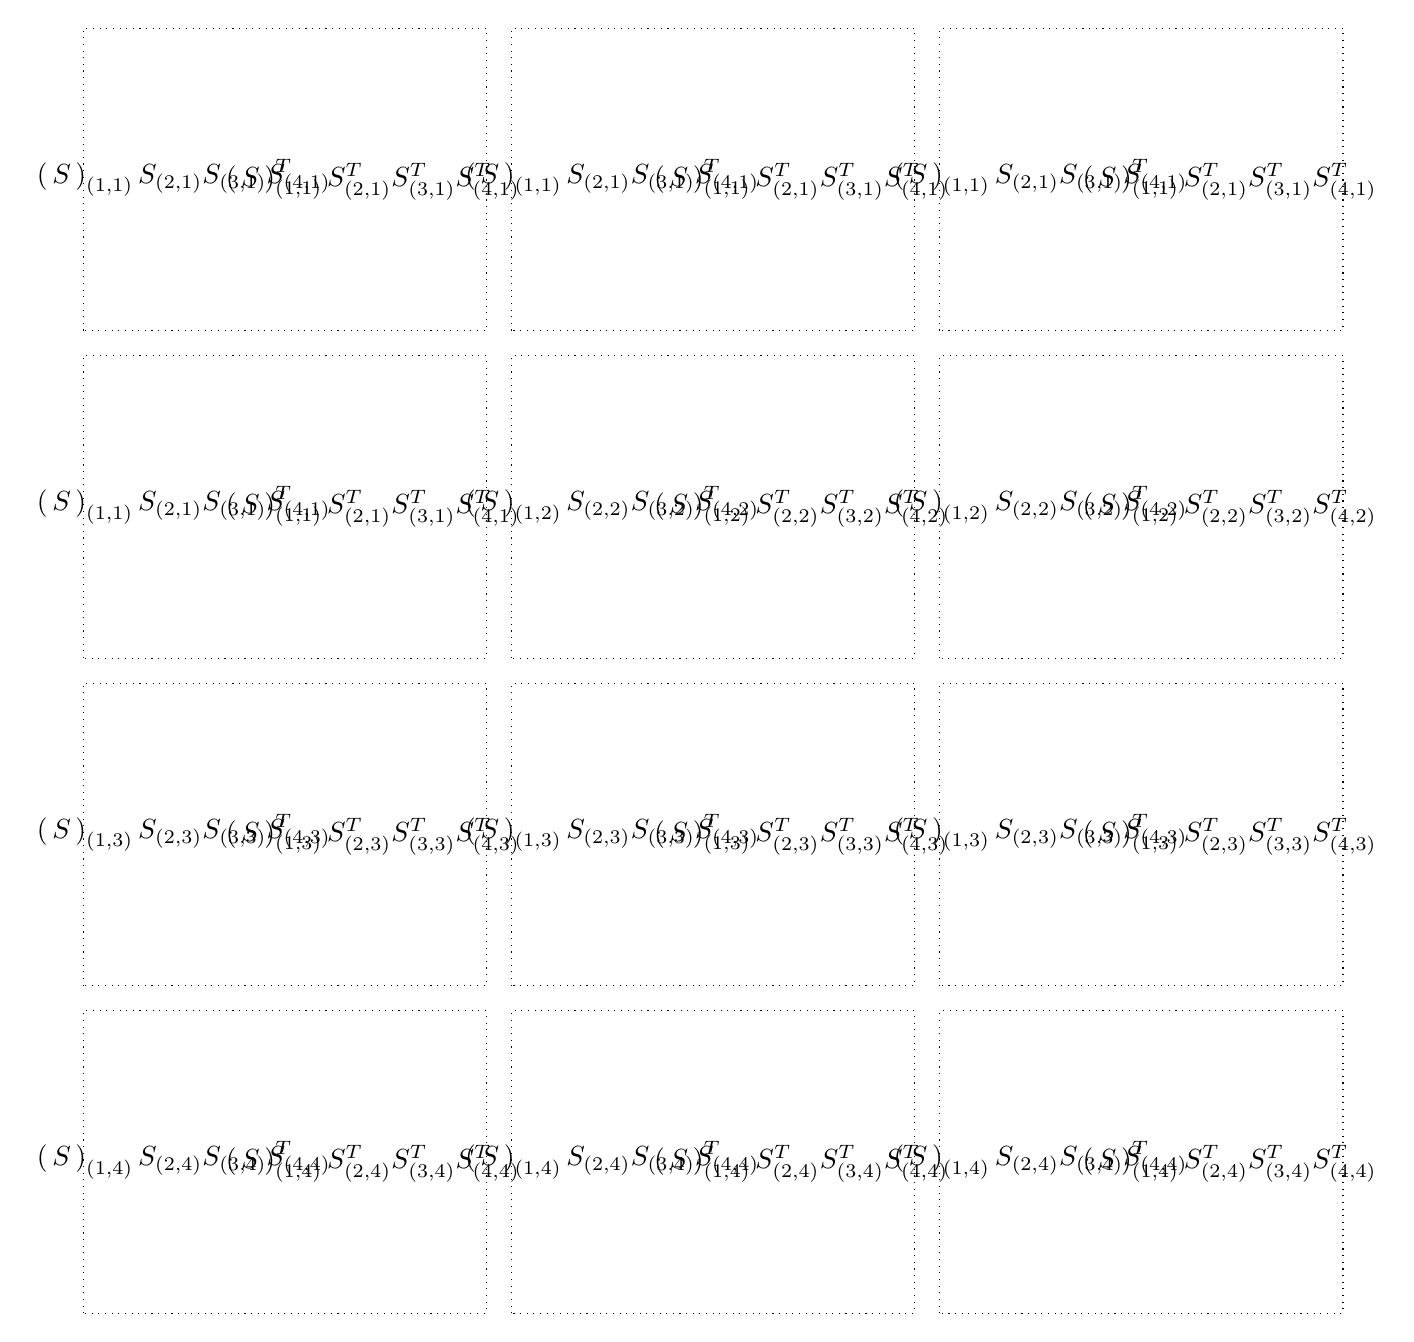
\begin{tikzpicture}[scale=16]
		% решетка процессов
		\draw [dotted] ( 0.00, 0.00 ) rectangle ( 0.32, 0.24 );
		\draw [dotted] ( 0.34, 0.00 ) rectangle ( 0.66, 0.24 );
		\draw [dotted] ( 0.68, 0.00 ) rectangle ( 1.00, 0.24 );
		\draw [dotted] ( 0.00, 0.26 ) rectangle ( 0.32, 0.50 );
		\draw [dotted] ( 0.34, 0.26 ) rectangle ( 0.66, 0.50 );
		\draw [dotted] ( 0.68, 0.26 ) rectangle ( 1.00, 0.50 );
		\draw [dotted] ( 0.00, 0.52 ) rectangle ( 0.32, 0.76 );
		\draw [dotted] ( 0.34, 0.52 ) rectangle ( 0.66, 0.76 );
		\draw [dotted] ( 0.68, 0.52 ) rectangle ( 1.00, 0.76 );
		\draw [dotted] ( 0.00, 0.78 ) rectangle ( 0.32, 1.02 );
		\draw [dotted] ( 0.34, 0.78 ) rectangle ( 0.66, 1.02 );
		\draw [dotted] ( 0.68, 0.78 ) rectangle ( 1.00, 1.02 );

		% процесс ( 1, 1 )
		\node at ( 0.08, 0.90 )	{ $ \begin{pmatrix} S_{(1,1)} \\ S_{(2,1)} \\ S_{(3,1)} \\ S_{(4,1)} \end{pmatrix} $ };
		\node at ( 0.23, 0.90 )	{ $ \begin{pmatrix}	S_{(1,1)}^T \\ S_{(2,1)}^T \\ S_{(3,1)}^T \\ S_{(4,1)}^T \end{pmatrix} $ };

		% процесс ( 1, 2 )
		\node at ( 0.42, 0.90 )	{ $ \begin{pmatrix} S_{(1,1)} \\ S_{(2,1)} \\ S_{(3,1)} \\ S_{(4,1)} \end{pmatrix} $ };
		\node at ( 0.57, 0.90 )	{ $ \begin{pmatrix}	S_{(1,1)}^T \\ S_{(2,1)}^T \\ S_{(3,1)}^T \\ S_{(4,1)}^T \end{pmatrix} $ };

		% процесс ( 1, 3 )
		\node at ( 0.76, 0.90 )	{ $ \begin{pmatrix} S_{(1,1)} \\ S_{(2,1)} \\ S_{(3,1)} \\ S_{(4,1)} \end{pmatrix} $ };
		\node at ( 0.91, 0.90 )	{ $ \begin{pmatrix}	S_{(1,1)}^T \\ S_{(2,1)}^T \\ S_{(3,1)}^T \\ S_{(4,1)}^T \end{pmatrix} $ };

		% процесс ( 2, 1 )
		\node at ( 0.08, 0.64 )	{ $ \begin{pmatrix} S_{(1,1)} \\ S_{(2,1)} \\ S_{(3,1)} \\ S_{(4,1)} \end{pmatrix} $ };
		\node at ( 0.23, 0.64 )	{ $ \begin{pmatrix}	S_{(1,1)}^T \\ S_{(2,1)}^T \\ S_{(3,1)}^T \\ S_{(4,1)}^T \end{pmatrix} $ };

		% процесс ( 2, 2 )
		\node at ( 0.42, 0.64 )	{ $ \begin{pmatrix} S_{(1,2)} \\ S_{(2,2)} \\ S_{(3,2)} \\ S_{(4,2)} \end{pmatrix} $ };
		\node at ( 0.57, 0.64 )	{ $ \begin{pmatrix}	S_{(1,2)}^T \\ S_{(2,2)}^T \\ S_{(3,2)}^T \\ S_{(4,2)}^T \end{pmatrix} $ };

		% процесс ( 2, 3 )
		\node at ( 0.76, 0.64 )	{ $ \begin{pmatrix} S_{(1,2)} \\ S_{(2,2)} \\ S_{(3,2)} \\ S_{(4,2)} \end{pmatrix} $ };
		\node at ( 0.91, 0.64 )	{ $ \begin{pmatrix}	S_{(1,2)}^T \\ S_{(2,2)}^T \\ S_{(3,2)}^T \\ S_{(4,2)}^T \end{pmatrix} $ };

		% процесс ( 3, 1 )
		\node at ( 0.08, 0.38 )	{ $ \begin{pmatrix} S_{(1,3)} \\ S_{(2,3)} \\ S_{(3,3)} \\ S_{(4,3)} \end{pmatrix} $ };
		\node at ( 0.23, 0.38 )	{ $ \begin{pmatrix}	S_{(1,3)}^T \\ S_{(2,3)}^T \\ S_{(3,3)}^T \\ S_{(4,3)}^T \end{pmatrix} $ };

		% процесс ( 3, 2 )
		\node at ( 0.42, 0.38 )	{ $ \begin{pmatrix} S_{(1,3)} \\ S_{(2,3)} \\ S_{(3,3)} \\ S_{(4,3)} \end{pmatrix} $ };
		\node at ( 0.57, 0.38 )	{ $ \begin{pmatrix}	S_{(1,3)}^T \\ S_{(2,3)}^T \\ S_{(3,3)}^T \\ S_{(4,3)}^T \end{pmatrix} $ };

		% процесс ( 3, 3 )
		\node at ( 0.76, 0.38 )	{ $ \begin{pmatrix} S_{(1,3)} \\ S_{(2,3)} \\ S_{(3,3)} \\ S_{(4,3)} \end{pmatrix} $ };
		\node at ( 0.91, 0.38 )	{ $ \begin{pmatrix}	S_{(1,3)}^T \\ S_{(2,3)}^T \\ S_{(3,3)}^T \\ S_{(4,3)}^T \end{pmatrix} $ };

		% процесс ( 4, 1 )
		\node at ( 0.08, 0.12 )	{ $ \begin{pmatrix} S_{(1,4)} \\ S_{(2,4)} \\ S_{(3,4)} \\ S_{(4,4)} \end{pmatrix} $ };
		\node at ( 0.23, 0.12 )	{ $ \begin{pmatrix}	S_{(1,4)}^T \\ S_{(2,4)}^T \\ S_{(3,4)}^T \\ S_{(4,4)}^T \end{pmatrix} $ };

		% процесс ( 4, 2 )
		\node at ( 0.42, 0.12 )	{ $ \begin{pmatrix} S_{(1,4)} \\ S_{(2,4)} \\ S_{(3,4)} \\ S_{(4,4)} \end{pmatrix} $ };
		\node at ( 0.57, 0.12 )	{ $ \begin{pmatrix}	S_{(1,4)}^T \\ S_{(2,4)}^T \\ S_{(3,4)}^T \\ S_{(4,4)}^T \end{pmatrix} $ };

		% процесс ( 4, 3 )
		\node at ( 0.76, 0.12 )	{ $ \begin{pmatrix} S_{(1,4)} \\ S_{(2,4)} \\ S_{(3,4)} \\ S_{(4,4)} \end{pmatrix} $ };
		\node at ( 0.91, 0.12 )	{ $ \begin{pmatrix}	S_{(1,4)}^T \\ S_{(2,4)}^T \\ S_{(3,4)}^T \\ S_{(4,4)}^T \end{pmatrix} $ };
	\end{tikzpicture}
	\caption{Распределение матриц $S$ и $S^T$}
	\label{figure:csmi:S_distribution}
\end{figure}

\subsection{Вычисление $V_i^{(S)} = S V_i$}

Основная идея вычисления $S V_i$ заключается в умножении с циклическими пересылками и подробно излагается в \cite{Zamarashkin}. Далее приводится изложение этой идеи
применительно к введенным обозначениям.

Блочный вектор $V_i^{(S)}$ распределяется между процессами так же как и блочный вектор $V_i$.
$$
	V_i^{(S)}
	=
	\begin{pmatrix}
		V_{i,(1,1)}^{(S)} & V_{i,(1,2)}^{(S)} & V_{i,(1,3)}^{(S)} \\
		V_{i,(2,1)}^{(S)} & V_{i,(2,2)}^{(S)} & V_{i,(2,3)}^{(S)} \\
		V_{i,(3,1)}^{(S)} & V_{i,(3,2)}^{(S)} & V_{i,(3,3)}^{(S)} \\
		V_{i,(4,1)}^{(S)} & V_{i,(4,2)}^{(S)} & V_{i,(4,3)}^{(S)}
	\end{pmatrix}
$$

Цель процесса с номером $[r,c]$ заключается в вычислении блока $V_{i,(r,c)}^{(S)}$.

Из представления умножения в блочной форме:
$$
	\begin{pmatrix}
		V_{i,(1,1)}^{(S)} & V_{i,(1,2)}^{(S)} & V_{i,(1,3)}^{(S)} \\
		V_{i,(2,1)}^{(S)} & V_{i,(2,2)}^{(S)} & V_{i,(2,3)}^{(S)} \\
		V_{i,(3,1)}^{(S)} & V_{i,(3,2)}^{(S)} & V_{i,(3,3)}^{(S)} \\
		V_{i,(4,1)}^{(S)} & V_{i,(4,2)}^{(S)} & V_{i,(4,3)}^{(S)}
	\end{pmatrix}
	=
	\begin{pmatrix}
		S_{(1,1)} & S_{(1,2)} & S_{(1,3)} & S_{(1,4)} \\
		S_{(2,1)} & S_{(2,2)} & S_{(2,3)} & S_{(2,4)} \\
		S_{(3,1)} & S_{(3,2)} & S_{(3,3)} & S_{(3,4)} \\
		S_{(4,1)} & S_{(4,2)} & S_{(4,3)} & S_{(4,4)}
	\end{pmatrix}
	\times
	\begin{pmatrix}
		V_{i,(1,1)} & V_{i,(1,2)} & V_{i,(1,3)} \\
		V_{i,(2,1)} & V_{i,(2,2)} & V_{i,(2,3)} \\
		V_{i,(3,1)} & V_{i,(3,2)} & V_{i,(3,3)} \\
		V_{i,(4,1)} & V_{i,(4,2)} & V_{i,(4,3)}
	\end{pmatrix}
$$
следует, что каждый блочный столбец $V_i^{(S)}$ с номером $c$, образованный блоками $V_{i,(\cdot,c)}^{(S)}$, может быть вычислен независимо от остальных блочных столбцов
$V_i^{(S)}$ с другими номерами, и для этого требуется лишь один блочный столбец $V_i$ с тем же номером $c$, образованный блоками $V_{i,(\cdot,c)}$. Поскольку вычисления блочных
столбцов $V_i^{(S)}$ являются однотипными, то далее рассматривается принцип вычисления применительно к столбцу с номером $c=1$:
$$
	\begin{pmatrix}
		V_{i,(1,1)}^{(S)} \\
		V_{i,(2,1)}^{(S)} \\
		V_{i,(3,1)}^{(S)} \\
		V_{i,(4,1)}^{(S)}
	\end{pmatrix}
	=
	\begin{pmatrix}
		S_{(1,1)} & S_{(1,2)} & S_{(1,3)} & S_{(1,4)} \\
		S_{(2,1)} & S_{(2,2)} & S_{(2,3)} & S_{(2,4)} \\
		S_{(3,1)} & S_{(3,2)} & S_{(3,3)} & S_{(3,4)} \\
		S_{(4,1)} & S_{(4,2)} & S_{(4,3)} & S_{(4,4)}
	\end{pmatrix}
	\times
	\begin{pmatrix}
		V_{i,(1,1)} \\
		V_{i,(2,1)} \\
		V_{i,(3,1)} \\
		V_{i,(4,1)}
	\end{pmatrix}
$$
Выполняя умножение в правой части, получим:
$$
	\begin{pmatrix}
		V_{i,(1,1)}^{(S)} \\
		V_{i,(2,1)}^{(S)} \\
		V_{i,(3,1)}^{(S)} \\
		V_{i,(4,1)}^{(S)}
	\end{pmatrix}
	=
	\begin{pmatrix}
		S_{(1,1)} V_{i,(1,1)} + S_{(1,2)} V_{i,(2,1)} + S_{(1,3)} V_{i,(3,1)} + S_{(1,4)} V_{i,(4,1)} \\
		S_{(2,1)} V_{i,(1,1)} + S_{(2,2)} V_{i,(2,1)} + S_{(2,3)} V_{i,(3,1)} + S_{(2,4)} V_{i,(4,1)} \\
		S_{(3,1)} V_{i,(1,1)} + S_{(3,2)} V_{i,(2,1)} + S_{(3,3)} V_{i,(3,1)} + S_{(3,4)} V_{i,(4,1)} \\
		S_{(4,1)} V_{i,(1,1)} + S_{(4,2)} V_{i,(2,1)} + S_{(4,3)} V_{i,(3,1)} + S_{(4,4)} V_{i,(4,1)}
	\end{pmatrix}
$$

Теперь рассмотрим какой-нибудь один процесс из первого столбца, например, с номером $r=2$, цель которого заключается в вычислении блока $V_{i,(2,1)}^{(S)}$. Легко видеть, что
для вычисления $V_{i,(2,1)}^{(S)}$ процессу $[2,1]$ требуется "собрать"\ сумму из четырех слагаемых:
$$
	V_{i,(2,1)}^{(S)}
	= \underbrace{S_{(2,1)} V_{i,(1,1)}}_1
	+ \underbrace{S_{(2,2)} V_{i,(2,1)}}_2
	+ \underbrace{S_{(2,3)} V_{i,(3,1)}}_3
	+ \underbrace{S_{(2,4)} V_{i,(4,1)}}_4
	,
$$
в которой процесс $[2,1]$ может вычислить только слагаемое $S_{(2,2)} V_{i,(2,1)}$ (оно обозначено цифрой 2), поскольку располагает блоком $V_{i,(2,1)}$, а остальные слагаемые
(обозначенные цифрами 1, 3, 4) вычислить не может: блоком $V_{i,(1,1)}$ располагает процесс $[1,1]$, блоком $V_{i,(3,1)}$ --- процесс $[3,1]$, а блоком $V_{i,(4,1)}$ ---
процесс $[4,1]$, поэтому слагаемые 1, 3 и 4 для процесса $[2,1]$ должны вычислить и прислать процессы $[1,1]$, $[3,1]$ и $[4,1]$.

Вообще говоря, точно такая же ситуация имеет место и во всех других процессах, которые могут вычислить только одно слагаемое в своей сумме, а остальные три слагамых должны
для них вычислить и прислать остальные три процесса.

Если преставить какие слагаемые может вычислить каждый из процессов, то получится следующий набор:
$$
	\begin{array}{cccc}
		1                     & 2                     & 3                     & 4 \\
		S_{(1,1)} V_{i,(1,1)} & S_{(1,2)} V_{i,(2,1)} & S_{(1,3)} V_{i,(3,1)} & S_{(1,4)} V_{i,(4,1)} \\
		S_{(2,1)} V_{i,(1,1)} & S_{(2,2)} V_{i,(2,1)} & S_{(2,3)} V_{i,(3,1)} & S_{(2,4)} V_{i,(4,1)} \\
		S_{(3,1)} V_{i,(1,1)} & S_{(3,2)} V_{i,(2,1)} & S_{(3,3)} V_{i,(3,1)} & S_{(3,4)} V_{i,(4,1)} \\
		S_{(4,1)} V_{i,(1,1)} & S_{(4,2)} V_{i,(2,1)} & S_{(4,3)} V_{i,(3,1)} & S_{(4,4)} V_{i,(4,1)}
	\end{array}
$$
в котором в первой строке указаны номера строк процессов (номер столбца у всех процессов равен 1 и опущен): 1 обозначает процесс $[1,1]$, 2 --- процесс $[2,1]$,
3 --- процесс $[3,1]$ и 4 --- процесс $[4,1]$.

Для того чтобы яснее представить себе идею умножения с циклическими пересылками необходимо столбцы с номерами 2, 3 и 4 переписать вперед
$$
	\begin{array}{ccccccc}
		2                     & 3                     & 4                     & 1                     & 2                     & 3                     & 4 \\
		S_{(1,2)} V_{i,(2,1)} & S_{(1,3)} V_{i,(3,1)} & S_{(1,4)} V_{i,(4,1)} & S_{(1,1)} V_{i,(1,1)} & S_{(1,2)} V_{i,(2,1)} & S_{(1,3)} V_{i,(3,1)} & S_{(1,4)} V_{i,(4,1)} \\
		S_{(2,2)} V_{i,(2,1)} & S_{(2,3)} V_{i,(3,1)} & S_{(2,4)} V_{i,(4,1)} & S_{(2,1)} V_{i,(1,1)} & S_{(2,2)} V_{i,(2,1)} & S_{(2,3)} V_{i,(3,1)} & S_{(2,4)} V_{i,(4,1)} \\
		S_{(3,2)} V_{i,(2,1)} & S_{(3,3)} V_{i,(3,1)} & S_{(3,4)} V_{i,(4,1)} & S_{(3,1)} V_{i,(1,1)} & S_{(3,2)} V_{i,(2,1)} & S_{(3,3)} V_{i,(3,1)} & S_{(3,4)} V_{i,(4,1)} \\
		S_{(4,2)} V_{i,(2,1)} & S_{(4,3)} V_{i,(3,1)} & S_{(4,4)} V_{i,(4,1)} & S_{(4,1)} V_{i,(1,1)} & S_{(4,2)} V_{i,(2,1)} & S_{(4,3)} V_{i,(3,1)} & S_{(4,4)} V_{i,(4,1)}
	\end{array}
$$
и убрать лишние слагаемые
$$
	\begin{array}{ccccccc}
		2                     & 3                     & 4                     & 1                     & 2                     & 3                     & 4 \\
		S_{(1,2)} V_{i,(2,1)} & S_{(1,3)} V_{i,(3,1)} & S_{(1,4)} V_{i,(4,1)} & S_{(1,1)} V_{i,(1,1)} &                       &                       & \\
		                      & S_{(2,3)} V_{i,(3,1)} & S_{(2,4)} V_{i,(4,1)} & S_{(2,1)} V_{i,(1,1)} & S_{(2,2)} V_{i,(2,1)} &                       & \\
		                      &                       & S_{(3,4)} V_{i,(4,1)} & S_{(3,1)} V_{i,(1,1)} & S_{(3,2)} V_{i,(2,1)} & S_{(3,3)} V_{i,(3,1)} & \\
		                      &                       &                       & S_{(4,1)} V_{i,(1,1)} & S_{(4,2)} V_{i,(2,1)} & S_{(4,3)} V_{i,(3,1)} & S_{(4,4)} V_{i,(4,1)}
	\end{array}
$$

Теперь, как легко видеть, во второй строке располагаются слагаемые, которые должен собрать процесс $[2,1]$, а в первой --- процесс $[1,1]$, в третьей --- процесс $[3,1]$,
а в четвертой --- процесс $[4,1]$. Числа над столбцами указывают какой процесс может вычислить это слагаемое. Вычисления необходимо проводить диагоналями слева направо.

Вычислять слагаемые для процессам $[2,1]$ начинает процесс $[3,1]$, он вычисляет слагаемое $S_{(2,3)} V_{i,(3,1)}$ (рисунок \ref{figure:csmi:S_V_step_1}) и
передает его "следующему"\ процессу $[4,1]$. Пока идет передача данных процесс $[4,1]$, не теряя времени, уже вычисляет следующее слагаемое для процесса $[2,1]$ --- блок
$S_{(2,4)} V_{i,(4,1)}$ (рисунок \ref{figure:csmi:S_V_step_2a}). Когда оба слагаемых будут получены в процессе $[4,1]$ он сможет сложить их
(рисунок \ref{figure:csmi:S_V_step_2b}). После сложения процесс $[4,1]$ может передать сумму из двух слагаемых "следующему"\ процессу $[1,1]$, который во время передачи данных
занимается вычислением следующего слагаемого для процесса $[2,1]$ --- блока $S_{(2,1)} V_{i,(1,1)}$ (рисунок \ref{figure:csmi:S_V_step_3a}). После получения суммы
из двух слагаемых процесс $[1,1]$ прибавляет вычисленный блок к принятой сумме (рисунок \ref{figure:csmi:S_V_step_3b}) и передает накопленную сумму уже из трех
слагаемых конечному процессу $[2,1]$ (рисунок \ref{figure:csmi:S_V_step_4a}). Процесс $[2,1]$ во время передачи данных вычисляет своё последнее слагаемое
$S_{(2,2)} V_{i,(2,1)}$ и прибавляет его к полученной сумме из трех слагаемых, тем самым, завершая вычисление своего блока $V_{i,(2,1)}^{(S)}$ (рисунок
\ref{figure:csmi:S_V_step_4b}).

Вычисление блоков $V_{i,(\cdot,1)}^{(S)}$ остальными процессами можно проследить по тем же рисункам.

\begin{figure}
	\begin{tikzpicture}[scale=16]
		% решетка процессов
		\draw [dotted] ( 0.00, 0.00 ) rectangle ( 0.32, 0.24 );
		\draw [dotted] ( 0.34, 0.00 ) rectangle ( 0.66, 0.24 );
		\draw [dotted] ( 0.68, 0.00 ) rectangle ( 1.00, 0.24 );
		\draw [dotted] ( 0.00, 0.26 ) rectangle ( 0.32, 0.50 );
		\draw [dotted] ( 0.34, 0.26 ) rectangle ( 0.66, 0.50 );
		\draw [dotted] ( 0.68, 0.26 ) rectangle ( 1.00, 0.50 );
		\draw [dotted] ( 0.00, 0.52 ) rectangle ( 0.32, 0.76 );
		\draw [dotted] ( 0.34, 0.52 ) rectangle ( 0.66, 0.76 );
		\draw [dotted] ( 0.68, 0.52 ) rectangle ( 1.00, 0.76 );
		\draw [dotted] ( 0.00, 0.78 ) rectangle ( 0.32, 1.02 );
		\draw [dotted] ( 0.34, 0.78 ) rectangle ( 0.66, 1.02 );
		\draw [dotted] ( 0.68, 0.78 ) rectangle ( 1.00, 1.02 );

		% процесс ( 1, 1 )
		\draw ( 0.13, 0.82 ) rectangle ( 0.15, 0.97 );
		\node [below right] at ( 0.15, 0.85 ) {$S_{(4,1)} V_{i,(1,1)}$};

		% процесс ( 1, 2 )
		\draw ( 0.47, 0.82 ) rectangle ( 0.49, 0.97 );
		\node [below right] at ( 0.49, 0.85 ) {$S_{(4,1)} V_{i,(1,2)}$};

		% процесс ( 1, 3 )
		\draw ( 0.81, 0.82 ) rectangle ( 0.83, 0.97 );
		\node [below right] at ( 0.83, 0.85 ) {$S_{(4,1)} V_{i,(1,3)}$};

		% процесс ( 2, 1 )
		\draw ( 0.13, 0.56 ) rectangle ( 0.15, 0.71 );
		\node [below right] at ( 0.15, 0.71 ) {$S_{(1,2)} V_{i,(2,1)}$};

		% процесс ( 2, 2 )
		\draw ( 0.47, 0.56 ) rectangle ( 0.49, 0.71 );
		\node [below right] at ( 0.49, 0.71 ) {$S_{(1,2)} V_{i,(2,2)}$};

		% процесс ( 2, 3 )
		\draw ( 0.81, 0.56 ) rectangle ( 0.83, 0.71 );
		\node [below right] at ( 0.83, 0.71 ) {$S_{(1,2)} V_{i,(2,3)}$};

		% процесс ( 3, 1 )
		\draw ( 0.13, 0.30 ) rectangle ( 0.15, 0.45 );
		\node [below right] at ( 0.15, 0.41 ) {$S_{(2,3)} V_{i,(3,1)}$};

		% процесс ( 3, 2 )
		\draw ( 0.47, 0.30 ) rectangle ( 0.49, 0.45 );
		\node [below right] at ( 0.49, 0.41 ) {$S_{(2,3)} V_{i,(3,2)}$};

		% процесс ( 3, 3 )
		\draw ( 0.81, 0.30 ) rectangle ( 0.83, 0.45 );
		\node [below right] at ( 0.83, 0.41 ) {$S_{(2,3)} V_{i,(3,3)}$};

		% процесс ( 4, 1 )
		\draw ( 0.13, 0.04 ) rectangle ( 0.15, 0.19 );
		\node [below right] at ( 0.15, 0.11 ) {$S_{(3,4)} V_{i,(4,1)}$};

		% процесс ( 4, 2 )
		\draw ( 0.47, 0.04 ) rectangle ( 0.49, 0.19 );
		\node [below right] at ( 0.49, 0.11 ) {$S_{(3,4)} V_{i,(4,2)}$};

		% процесс ( 4, 3 )
		\draw ( 0.81, 0.04 ) rectangle ( 0.83, 0.19 );
		\node [below right] at ( 0.83, 0.11 ) {$S_{(3,4)} V_{i,(4,3)}$};
	\end{tikzpicture}
	\caption{Вычисление $V_i^{(S)} = S V_i$: шаг 1}
	\label{figure:csmi:S_V_step_1}
\end{figure}

\begin{figure}
	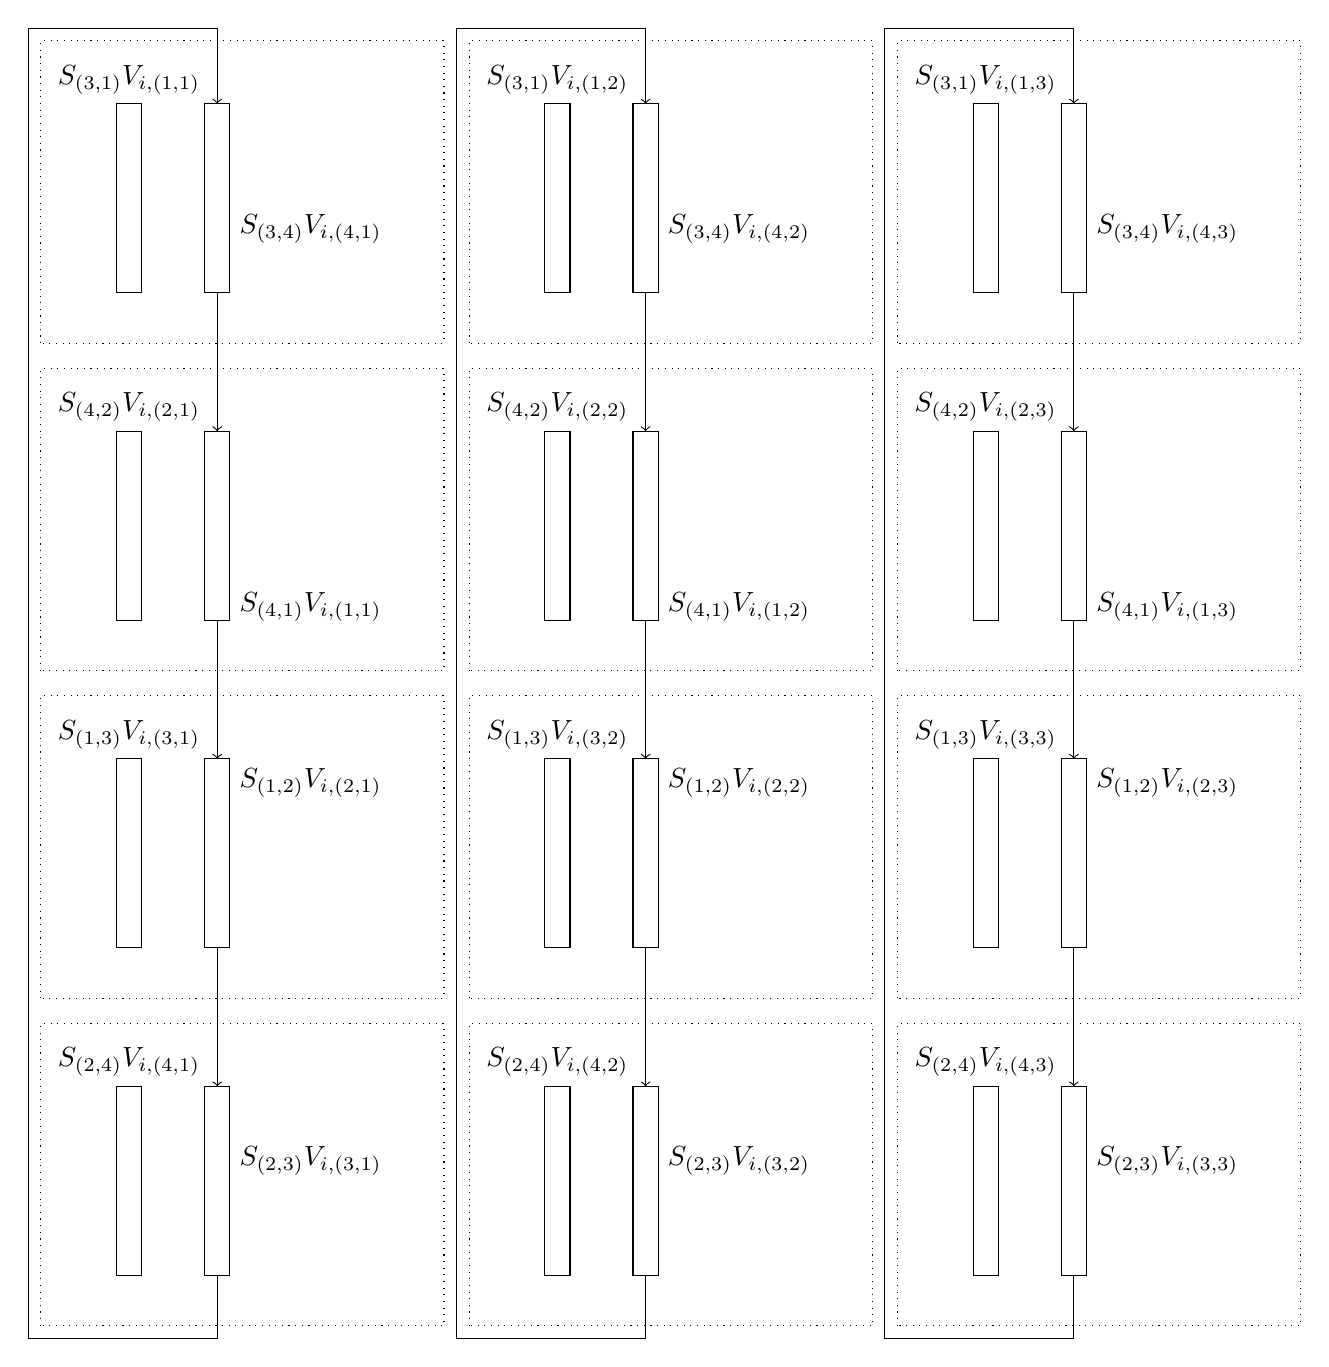
\begin{tikzpicture}[scale=16]
		% решетка процессов
		\draw [dotted] ( 0.00, 0.00 ) rectangle ( 0.32, 0.24 );
		\draw [dotted] ( 0.34, 0.00 ) rectangle ( 0.66, 0.24 );
		\draw [dotted] ( 0.68, 0.00 ) rectangle ( 1.00, 0.24 );
		\draw [dotted] ( 0.00, 0.26 ) rectangle ( 0.32, 0.50 );
		\draw [dotted] ( 0.34, 0.26 ) rectangle ( 0.66, 0.50 );
		\draw [dotted] ( 0.68, 0.26 ) rectangle ( 1.00, 0.50 );
		\draw [dotted] ( 0.00, 0.52 ) rectangle ( 0.32, 0.76 );
		\draw [dotted] ( 0.34, 0.52 ) rectangle ( 0.66, 0.76 );
		\draw [dotted] ( 0.68, 0.52 ) rectangle ( 1.00, 0.76 );
		\draw [dotted] ( 0.00, 0.78 ) rectangle ( 0.32, 1.02 );
		\draw [dotted] ( 0.34, 0.78 ) rectangle ( 0.66, 1.02 );
		\draw [dotted] ( 0.68, 0.78 ) rectangle ( 1.00, 1.02 );

		% процесс ( 1, 1 )
		\draw ( 0.06, 0.82 ) rectangle ( 0.08, 0.97 ) node [above] at ( 0.07, 0.97 ) {$S_{(3,1)} V_{i,(1,1)}$};
		\draw ( 0.13, 0.82 ) rectangle ( 0.15, 0.97 );
		\node [below right] at ( 0.15, 0.89 ) {$S_{(3,4)} V_{i,(4,1)}$};
		\draw [->] ( 0.14, 0.82 ) -- ( 0.14, 0.71 );

		% процесс ( 1, 2 )
		\draw ( 0.40, 0.82 ) rectangle ( 0.42, 0.97 ) node [above] at ( 0.41, 0.97 ) {$S_{(3,1)} V_{i,(1,2)}$};
		\draw ( 0.47, 0.82 ) rectangle ( 0.49, 0.97 );
		\node [below right] at ( 0.49, 0.89 ) {$S_{(3,4)} V_{i,(4,2)}$};
		\draw [->] ( 0.48, 0.82 ) -- ( 0.48, 0.71 );

		% процесс ( 1, 3 )
		\draw ( 0.74, 0.82 ) rectangle ( 0.76, 0.97 ) node [above] at ( 0.75, 0.97 ) {$S_{(3,1)} V_{i,(1,3)}$};
		\draw ( 0.81, 0.82 ) rectangle ( 0.83, 0.97 );
		\node [below right] at ( 0.83, 0.89 ) {$S_{(3,4)} V_{i,(4,3)}$};
		\draw [->] ( 0.82, 0.82 ) -- ( 0.82, 0.71 );

		% процесс ( 2, 1 )
		\draw ( 0.06, 0.56 ) rectangle ( 0.08, 0.71 ) node [above] at ( 0.07, 0.71 ) {$S_{(4,2)} V_{i,(2,1)}$};
		\draw ( 0.13, 0.56 ) rectangle ( 0.15, 0.71 );
		\node [below right] at ( 0.15, 0.59 ) {$S_{(4,1)} V_{i,(1,1)}$};
		\draw [->] ( 0.14, 0.56 ) -- ( 0.14, 0.45 );

		% процесс ( 2, 2 )
		\draw ( 0.40, 0.56 ) rectangle ( 0.42, 0.71 ) node [above] at ( 0.41, 0.71 ) {$S_{(4,2)} V_{i,(2,2)}$};
		\draw ( 0.47, 0.56 ) rectangle ( 0.49, 0.71 );
		\node [below right] at ( 0.49, 0.59 ) {$S_{(4,1)} V_{i,(1,2)}$};
		\draw [->] ( 0.48, 0.56 ) -- ( 0.48, 0.45 );

		% процесс ( 2, 3 )
		\draw ( 0.74, 0.56 ) rectangle ( 0.76, 0.71 ) node [above] at ( 0.75, 0.71 ) {$S_{(4,2)} V_{i,(2,3)}$};
		\draw ( 0.81, 0.56 ) rectangle ( 0.83, 0.71 );
		\node [below right] at ( 0.83, 0.59 ) {$S_{(4,1)} V_{i,(1,3)}$};
		\draw [->] ( 0.82, 0.56 ) -- ( 0.82, 0.45 );

		% процесс ( 3, 1 )
		\draw ( 0.06, 0.30 ) rectangle ( 0.08, 0.45 ) node [above] at ( 0.07, 0.45 ) {$S_{(1,3)} V_{i,(3,1)}$};
		\draw ( 0.13, 0.30 ) rectangle ( 0.15, 0.45 );
		\node [below right] at ( 0.15, 0.45 ) {$S_{(1,2)} V_{i,(2,1)}$};
		\draw [->] ( 0.14, 0.30 ) -- ( 0.14, 0.19 );

		% процесс ( 3, 2 )
		\draw ( 0.40, 0.30 ) rectangle ( 0.42, 0.45 ) node [above] at ( 0.41, 0.45 ) {$S_{(1,3)} V_{i,(3,2)}$};
		\draw ( 0.47, 0.30 ) rectangle ( 0.49, 0.45 );
		\node [below right] at ( 0.49, 0.45 ) {$S_{(1,2)} V_{i,(2,2)}$};
		\draw [->] ( 0.48, 0.30 ) -- ( 0.48, 0.19 );

		% процесс ( 3, 3 )
		\draw ( 0.74, 0.30 ) rectangle ( 0.76, 0.45 ) node [above] at ( 0.75, 0.45 ) {$S_{(1,3)} V_{i,(3,3)}$};
		\draw ( 0.81, 0.30 ) rectangle ( 0.83, 0.45 );
		\node [below right] at ( 0.83, 0.45 ) {$S_{(1,2)} V_{i,(2,3)}$};
		\draw [->] ( 0.82, 0.30 ) -- ( 0.82, 0.19 );

		% процесс ( 4, 1 )
		\draw ( 0.06, 0.04 ) rectangle ( 0.08, 0.19 ) node [above] at ( 0.07, 0.19 ) {$S_{(2,4)} V_{i,(4,1)}$};
		\draw ( 0.13, 0.04 ) rectangle ( 0.15, 0.19 );
		\node [below right] at ( 0.15, 0.15 ) {$S_{(2,3)} V_{i,(3,1)}$};
		\draw [->] ( 0.14, 0.04 ) -- ( 0.14, -0.01 ) -- ( -0.01, -0.01 ) -- ( -0.01, 1.03 ) -- ( 0.14, 1.03 ) -- ( 0.14, 0.97 );

		% процесс ( 4, 2 )
		\draw ( 0.40, 0.04 ) rectangle ( 0.42, 0.19 ) node [above] at ( 0.41, 0.19 ) {$S_{(2,4)} V_{i,(4,2)}$};
		\draw ( 0.47, 0.04 ) rectangle ( 0.49, 0.19 );
		\node [below right] at ( 0.49, 0.15 ) {$S_{(2,3)} V_{i,(3,2)}$};
		\draw [->] ( 0.48, 0.04 ) -- ( 0.48, -0.01 ) -- ( 0.33, -0.01 ) -- ( 0.33, 1.03 ) -- ( 0.48, 1.03 ) -- ( 0.48, 0.97 );

		% процесс ( 4, 3 )
		\draw ( 0.74, 0.04 ) rectangle ( 0.76, 0.19 ) node [above] at ( 0.75, 0.19 ) {$S_{(2,4)} V_{i,(4,3)}$};
		\draw ( 0.81, 0.04 ) rectangle ( 0.83, 0.19 );
		\node [below right] at ( 0.83, 0.15 ) {$S_{(2,3)} V_{i,(3,3)}$};
		\draw [->] ( 0.82, 0.04 ) -- ( 0.82, -0.01 ) -- ( 0.67, -0.01 ) -- ( 0.67, 1.03 ) -- ( 0.82, 1.03 ) -- ( 0.82, 0.97 );
	\end{tikzpicture}
	\caption{Вычисление $V_i^{(S)} = S V_i$: шаг 2а}
	\label{figure:csmi:S_V_step_2a}
\end{figure}

\begin{figure}
	\begin{tikzpicture}[scale=16]
		% решетка процессов
		\draw [dotted] ( 0.00, 0.00 ) rectangle ( 0.32, 0.24 );
		\draw [dotted] ( 0.34, 0.00 ) rectangle ( 0.66, 0.24 );
		\draw [dotted] ( 0.68, 0.00 ) rectangle ( 1.00, 0.24 );
		\draw [dotted] ( 0.00, 0.26 ) rectangle ( 0.32, 0.50 );
		\draw [dotted] ( 0.34, 0.26 ) rectangle ( 0.66, 0.50 );
		\draw [dotted] ( 0.68, 0.26 ) rectangle ( 1.00, 0.50 );
		\draw [dotted] ( 0.00, 0.52 ) rectangle ( 0.32, 0.76 );
		\draw [dotted] ( 0.34, 0.52 ) rectangle ( 0.66, 0.76 );
		\draw [dotted] ( 0.68, 0.52 ) rectangle ( 1.00, 0.76 );
		\draw [dotted] ( 0.00, 0.78 ) rectangle ( 0.32, 1.02 );
		\draw [dotted] ( 0.34, 0.78 ) rectangle ( 0.66, 1.02 );
		\draw [dotted] ( 0.68, 0.78 ) rectangle ( 1.00, 1.02 );

		% процесс ( 1, 1 )
		\draw ( 0.13, 0.82 ) rectangle ( 0.15, 0.97 );
		\node [below right] at ( 0.15, 0.97 ) {$S_{(3,1)} V_{i,(1,1)}$};
		\node [below right] at ( 0.15, 0.89 ) {$+ S_{(3,4)} V_{i,(4,1)}$};

		% процесс ( 1, 2 )
		\draw ( 0.47, 0.82 ) rectangle ( 0.49, 0.97 );
		\node [below right] at ( 0.49, 0.97 ) {$S_{(3,1)} V_{i,(1,2)}$};
		\node [below right] at ( 0.49, 0.89 ) {$+ S_{(3,4)} V_{i,(4,2)}$};

		% процесс ( 1, 3 )
		\draw ( 0.81, 0.82 ) rectangle ( 0.83, 0.97 );
		\node [below right] at ( 0.83, 0.97 ) {$S_{(3,1)} V_{i,(1,3)}$};
		\node [below right] at ( 0.83, 0.89 ) {$+ S_{(3,4)} V_{i,(4,3)}$};

		% процесс ( 2, 1 )
		\draw ( 0.13, 0.56 ) rectangle ( 0.15, 0.71 );
		\node [below right] at ( 0.15, 0.71 ) {$S_{(4,1)} V_{i,(1,1)}$};
		\node [below right] at ( 0.15, 0.67 ) {$+ S_{(4,2)} V_{i,(2,1)}$};

		% процесс ( 2, 2 )
		\draw ( 0.47, 0.56 ) rectangle ( 0.49, 0.71 );
		\node [below right] at ( 0.49, 0.71 ) {$S_{(4,1)} V_{i,(1,2)}$};
		\node [below right] at ( 0.49, 0.67 ) {$+ S_{(4,2)} V_{i,(2,2)}$};

		% процесс ( 2, 3 )
		\draw ( 0.81, 0.56 ) rectangle ( 0.83, 0.71 );
		\node [below right] at ( 0.83, 0.71 ) {$S_{(4,1)} V_{i,(1,3)}$};
		\node [below right] at ( 0.83, 0.67 ) {$+ S_{(4,2)} V_{i,(2,3)}$};

		% процесс ( 3, 1 )
		\draw ( 0.13, 0.30 ) rectangle ( 0.15, 0.45 );
		\node [below right] at ( 0.15, 0.41 ) {$S_{(1,2)} V_{i,(2,1)}$};
		\node [below right] at ( 0.15, 0.37 ) {$+ S_{(1,3)} V_{i,(3,1)}$};

		% процесс ( 3, 2 )
		\draw ( 0.47, 0.30 ) rectangle ( 0.49, 0.45 );
		\node [below right] at ( 0.49, 0.41 ) {$S_{(1,2)} V_{i,(2,2)}$};
		\node [below right] at ( 0.49, 0.37 ) {$+ S_{(1,3)} V_{i,(3,2)}$};

		% процесс ( 3, 3 )
		\draw ( 0.81, 0.30 ) rectangle ( 0.83, 0.45 );
		\node [below right] at ( 0.83, 0.41 ) {$S_{(1,2)} V_{i,(2,3)}$};
		\node [below right] at ( 0.83, 0.37 ) {$+ S_{(1,3)} V_{i,(3,3)}$};

		% процесс ( 4, 1 )
		\draw ( 0.13, 0.04 ) rectangle ( 0.15, 0.19 );
		\node [below right] at ( 0.15, 0.11 ) {$S_{(2,3)} V_{i,(3,1)}$};
		\node [below right] at ( 0.15, 0.07 ) {$+ S_{(2,4)} V_{i,(4,1)}$};

		% процесс ( 4, 2 )
		\draw ( 0.47, 0.04 ) rectangle ( 0.49, 0.19 );
		\node [below right] at ( 0.49, 0.11 ) {$S_{(2,3)} V_{i,(3,2)}$};
		\node [below right] at ( 0.49, 0.07 ) {$+ S_{(2,4)} V_{i,(4,2)}$};

		% процесс ( 4, 3 )
		\draw ( 0.81, 0.04 ) rectangle ( 0.83, 0.19 );
		\node [below right] at ( 0.83, 0.11 ) {$S_{(2,3)} V_{i,(3,3)}$};
		\node [below right] at ( 0.83, 0.07 ) {$+ S_{(2,4)} V_{i,(4,3)}$};
	\end{tikzpicture}
	\caption{Вычисление $V_i^{(S)} = S V_i$: шаг 2б}
	\label{figure:csmi:S_V_step_2b}
\end{figure}

\begin{figure}
	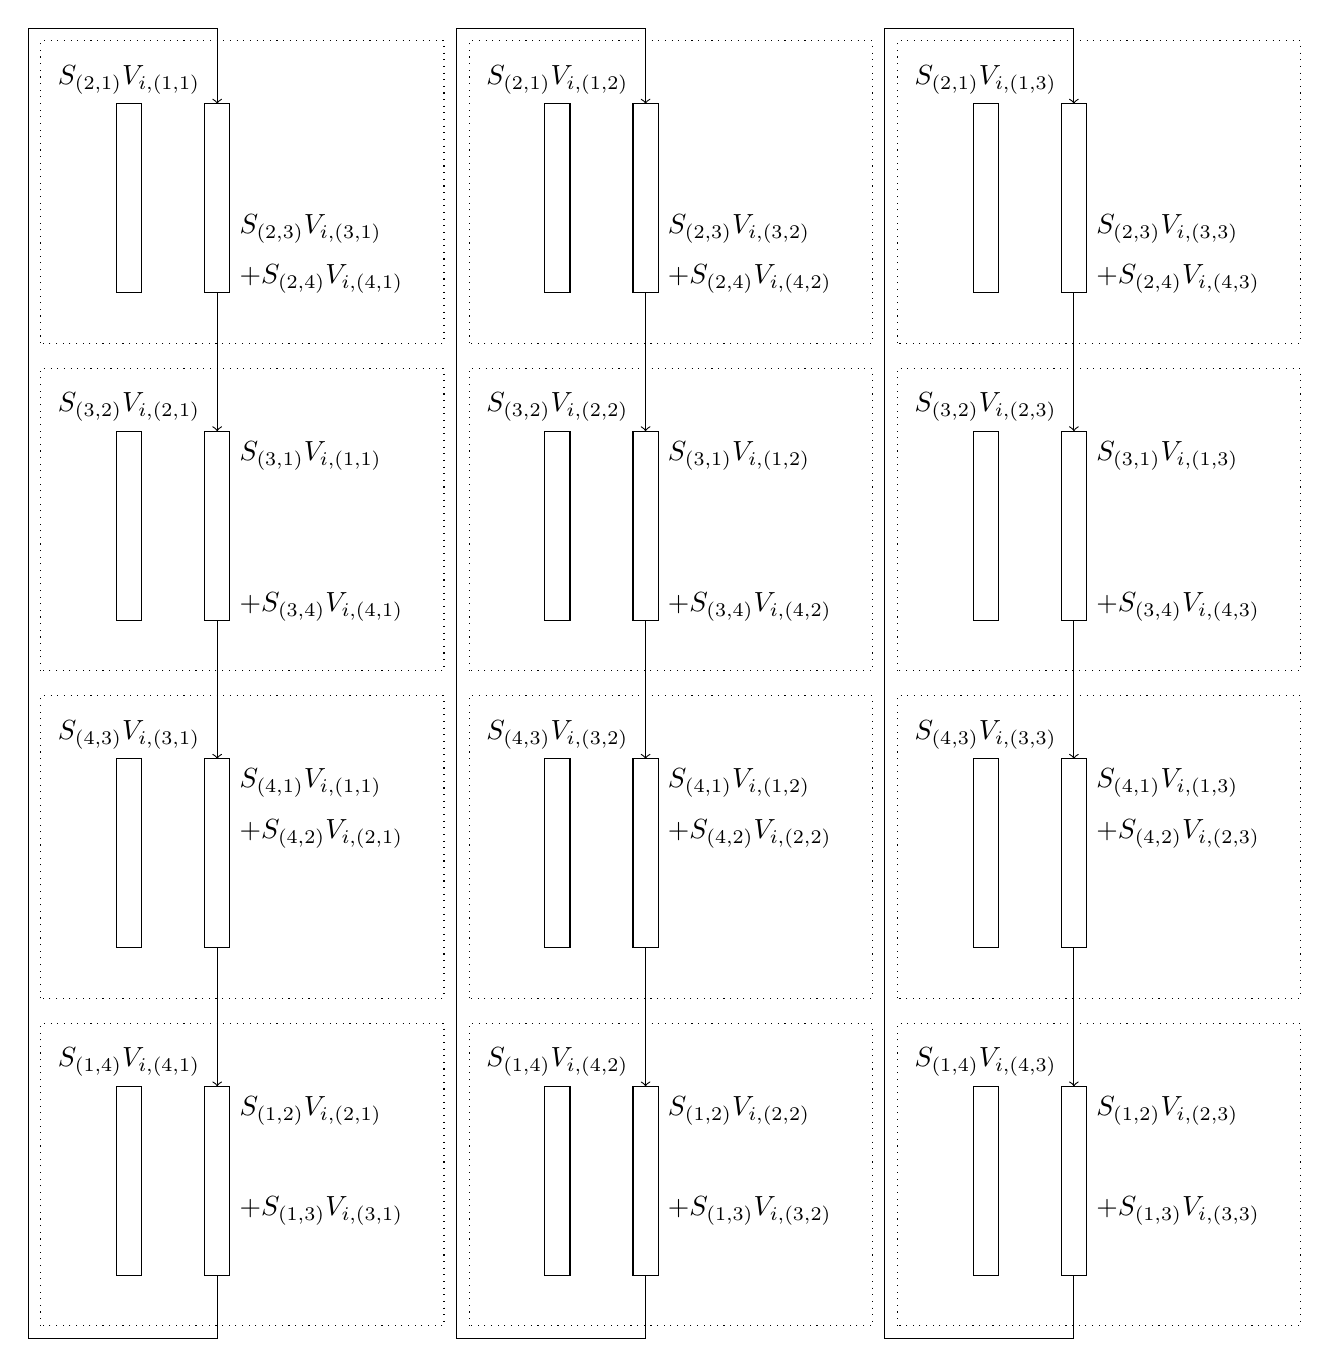
\begin{tikzpicture}[scale=16]
		% решетка процессов
		\draw [dotted] ( 0.00, 0.00 ) rectangle ( 0.32, 0.24 );
		\draw [dotted] ( 0.34, 0.00 ) rectangle ( 0.66, 0.24 );
		\draw [dotted] ( 0.68, 0.00 ) rectangle ( 1.00, 0.24 );
		\draw [dotted] ( 0.00, 0.26 ) rectangle ( 0.32, 0.50 );
		\draw [dotted] ( 0.34, 0.26 ) rectangle ( 0.66, 0.50 );
		\draw [dotted] ( 0.68, 0.26 ) rectangle ( 1.00, 0.50 );
		\draw [dotted] ( 0.00, 0.52 ) rectangle ( 0.32, 0.76 );
		\draw [dotted] ( 0.34, 0.52 ) rectangle ( 0.66, 0.76 );
		\draw [dotted] ( 0.68, 0.52 ) rectangle ( 1.00, 0.76 );
		\draw [dotted] ( 0.00, 0.78 ) rectangle ( 0.32, 1.02 );
		\draw [dotted] ( 0.34, 0.78 ) rectangle ( 0.66, 1.02 );
		\draw [dotted] ( 0.68, 0.78 ) rectangle ( 1.00, 1.02 );

		% процесс ( 1, 1 )
		\draw ( 0.06, 0.82 ) rectangle ( 0.08, 0.97 ) node [above] at ( 0.07, 0.97 ) {$S_{(2,1)} V_{i,(1,1)}$};
		\draw ( 0.13, 0.82 ) rectangle ( 0.15, 0.97 );
		\node [below right] at ( 0.15, 0.89 ) {$S_{(2,3)} V_{i,(3,1)}$};
		\node [below right] at ( 0.15, 0.85 ) {$+ S_{(2,4)} V_{i,(4,1)}$};
		\draw [->] ( 0.14, 0.82 ) -- ( 0.14, 0.71 );

		% процесс ( 1, 2 )
		\draw ( 0.40, 0.82 ) rectangle ( 0.42, 0.97 ) node [above] at ( 0.41, 0.97 ) {$S_{(2,1)} V_{i,(1,2)}$};
		\draw ( 0.47, 0.82 ) rectangle ( 0.49, 0.97 );
		\node [below right] at ( 0.49, 0.89 ) {$S_{(2,3)} V_{i,(3,2)}$};
		\node [below right] at ( 0.49, 0.85 ) {$+ S_{(2,4)} V_{i,(4,2)}$};
		\draw [->] ( 0.48, 0.82 ) -- ( 0.48, 0.71 );

		% процесс ( 1, 3 )
		\draw ( 0.74, 0.82 ) rectangle ( 0.76, 0.97 ) node [above] at ( 0.75, 0.97 ) {$S_{(2,1)} V_{i,(1,3)}$};
		\draw ( 0.81, 0.82 ) rectangle ( 0.83, 0.97 );
		\node [below right] at ( 0.83, 0.89 ) {$S_{(2,3)} V_{i,(3,3)}$};
		\node [below right] at ( 0.83, 0.85 ) {$+ S_{(2,4)} V_{i,(4,3)}$};
		\draw [->] ( 0.82, 0.82 ) -- ( 0.82, 0.71 );

		% процесс ( 2, 1 )
		\draw ( 0.06, 0.56 ) rectangle ( 0.08, 0.71 ) node [above] at ( 0.07, 0.71 ) {$S_{(3,2)} V_{i,(2,1)}$};
		\draw ( 0.13, 0.56 ) rectangle ( 0.15, 0.71 );
		\node [below right] at ( 0.15, 0.71 ) {$S_{(3,1)} V_{i,(1,1)}$};
		\node [below right] at ( 0.15, 0.59 ) {$+ S_{(3,4)} V_{i,(4,1)}$};
		\draw [->] ( 0.14, 0.56 ) -- ( 0.14, 0.45 );

		% процесс ( 2, 2 )
		\draw ( 0.40, 0.56 ) rectangle ( 0.42, 0.71 ) node [above] at ( 0.41, 0.71 ) {$S_{(3,2)} V_{i,(2,2)}$};
		\draw ( 0.47, 0.56 ) rectangle ( 0.49, 0.71 );
		\node [below right] at ( 0.49, 0.71 ) {$S_{(3,1)} V_{i,(1,2)}$};
		\node [below right] at ( 0.49, 0.59 ) {$+ S_{(3,4)} V_{i,(4,2)}$};
		\draw [->] ( 0.48, 0.56 ) -- ( 0.48, 0.45 );

		% процесс ( 2, 3 )
		\draw ( 0.74, 0.56 ) rectangle ( 0.76, 0.71 ) node [above] at ( 0.75, 0.71 ) {$S_{(3,2)} V_{i,(2,3)}$};
		\draw ( 0.81, 0.56 ) rectangle ( 0.83, 0.71 );
		\node [below right] at ( 0.83, 0.71 ) {$S_{(3,1)} V_{i,(1,3)}$};
		\node [below right] at ( 0.83, 0.59 ) {$+ S_{(3,4)} V_{i,(4,3)}$};
		\draw [->] ( 0.82, 0.56 ) -- ( 0.82, 0.45 );

		% процесс ( 3, 1 )
		\draw ( 0.06, 0.30 ) rectangle ( 0.08, 0.45 ) node [above] at ( 0.07, 0.45 ) {$S_{(4,3)} V_{i,(3,1)}$};
		\draw ( 0.13, 0.30 ) rectangle ( 0.15, 0.45 );
		\node [below right] at ( 0.15, 0.45 ) {$S_{(4,1)} V_{i,(1,1)}$};
		\node [below right] at ( 0.15, 0.41 ) {$+ S_{(4,2)} V_{i,(2,1)}$};
		\draw [->] ( 0.14, 0.30 ) -- ( 0.14, 0.19 );

		% процесс ( 3, 2 )
		\draw ( 0.40, 0.30 ) rectangle ( 0.42, 0.45 ) node [above] at ( 0.41, 0.45 ) {$S_{(4,3)} V_{i,(3,2)}$};
		\draw ( 0.47, 0.30 ) rectangle ( 0.49, 0.45 );
		\node [below right] at ( 0.49, 0.45 ) {$S_{(4,1)} V_{i,(1,2)}$};
		\node [below right] at ( 0.49, 0.41 ) {$+ S_{(4,2)} V_{i,(2,2)}$};
		\draw [->] ( 0.48, 0.30 ) -- ( 0.48, 0.19 );

		% процесс ( 3, 3 )
		\draw ( 0.74, 0.30 ) rectangle ( 0.76, 0.45 ) node [above] at ( 0.75, 0.45 ) {$S_{(4,3)} V_{i,(3,3)}$};
		\draw ( 0.81, 0.30 ) rectangle ( 0.83, 0.45 );
		\node [below right] at ( 0.83, 0.45 ) {$S_{(4,1)} V_{i,(1,3)}$};
		\node [below right] at ( 0.83, 0.41 ) {$+ S_{(4,2)} V_{i,(2,3)}$};
		\draw [->] ( 0.82, 0.30 ) -- ( 0.82, 0.19 );

		% процесс ( 4, 1 )
		\draw ( 0.06, 0.04 ) rectangle ( 0.08, 0.19 ) node [above] at ( 0.07, 0.19 ) {$S_{(1,4)} V_{i,(4,1)}$};
		\draw ( 0.13, 0.04 ) rectangle ( 0.15, 0.19 );
		\node [below right] at ( 0.15, 0.19 ) {$S_{(1,2)} V_{i,(2,1)}$};
		\node [below right] at ( 0.15, 0.11 ) {$+ S_{(1,3)} V_{i,(3,1)}$};
		\draw [->] ( 0.14, 0.04 ) -- ( 0.14, -0.01 ) -- ( -0.01, -0.01 ) -- ( -0.01, 1.03 ) -- ( 0.14, 1.03 ) -- ( 0.14, 0.97 );

		% процесс ( 4, 2 )
		\draw ( 0.40, 0.04 ) rectangle ( 0.42, 0.19 ) node [above] at ( 0.41, 0.19 ) {$S_{(1,4)} V_{i,(4,2)}$};
		\draw ( 0.47, 0.04 ) rectangle ( 0.49, 0.19 );
		\node [below right] at ( 0.49, 0.19 ) {$S_{(1,2)} V_{i,(2,2)}$};
		\node [below right] at ( 0.49, 0.11 ) {$+ S_{(1,3)} V_{i,(3,2)}$};
		\draw [->] ( 0.48, 0.04 ) -- ( 0.48, -0.01 ) -- ( 0.33, -0.01 ) -- ( 0.33, 1.03 ) -- ( 0.48, 1.03 ) -- ( 0.48, 0.97 );

		% процесс ( 4, 3 )
		\draw ( 0.74, 0.04 ) rectangle ( 0.76, 0.19 ) node [above] at ( 0.75, 0.19 ) {$S_{(1,4)} V_{i,(4,3)}$};
		\draw ( 0.81, 0.04 ) rectangle ( 0.83, 0.19 );
		\node [below right] at ( 0.83, 0.19 ) {$S_{(1,2)} V_{i,(2,3)}$};
		\node [below right] at ( 0.83, 0.11 ) {$+ S_{(1,3)} V_{i,(3,3)}$};
		\draw [->] ( 0.82, 0.04 ) -- ( 0.82, -0.01 ) -- ( 0.67, -0.01 ) -- ( 0.67, 1.03 ) -- ( 0.82, 1.03 ) -- ( 0.82, 0.97 );
	\end{tikzpicture}
	\caption{Вычисление $V_i^{(S)} = S V_i$: шаг 3a}
	\label{figure:csmi:S_V_step_3a}
\end{figure}

\begin{figure}
	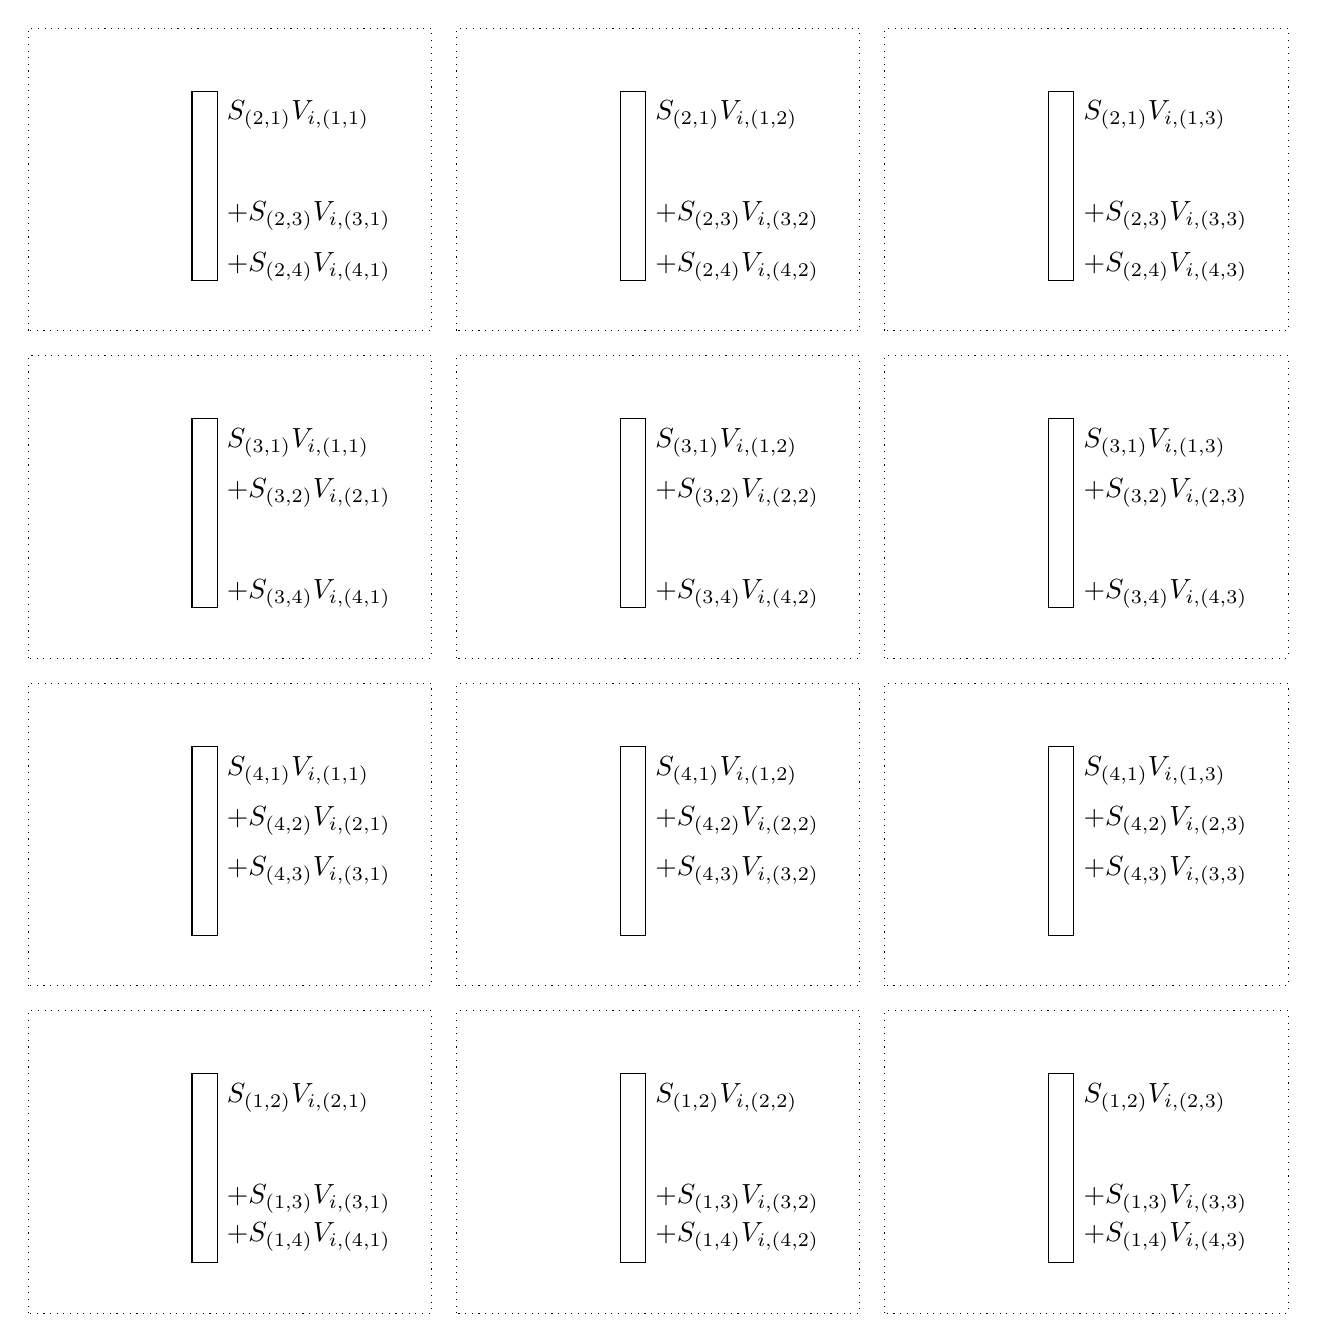
\begin{tikzpicture}[scale=16]
		% решетка процессов
		\draw [dotted] ( 0.00, 0.00 ) rectangle ( 0.32, 0.24 );
		\draw [dotted] ( 0.34, 0.00 ) rectangle ( 0.66, 0.24 );
		\draw [dotted] ( 0.68, 0.00 ) rectangle ( 1.00, 0.24 );
		\draw [dotted] ( 0.00, 0.26 ) rectangle ( 0.32, 0.50 );
		\draw [dotted] ( 0.34, 0.26 ) rectangle ( 0.66, 0.50 );
		\draw [dotted] ( 0.68, 0.26 ) rectangle ( 1.00, 0.50 );
		\draw [dotted] ( 0.00, 0.52 ) rectangle ( 0.32, 0.76 );
		\draw [dotted] ( 0.34, 0.52 ) rectangle ( 0.66, 0.76 );
		\draw [dotted] ( 0.68, 0.52 ) rectangle ( 1.00, 0.76 );
		\draw [dotted] ( 0.00, 0.78 ) rectangle ( 0.32, 1.02 );
		\draw [dotted] ( 0.34, 0.78 ) rectangle ( 0.66, 1.02 );
		\draw [dotted] ( 0.68, 0.78 ) rectangle ( 1.00, 1.02 );

		% процесс ( 1, 1 )
		\draw ( 0.13, 0.82 ) rectangle ( 0.15, 0.97 );
 		\node [below right] at ( 0.15, 0.97 ) {$S_{(2,1)} V_{i,(1,1)}$};
		\node [below right] at ( 0.15, 0.89 ) {$+ S_{(2,3)} V_{i,(3,1)}$};
 		\node [below right] at ( 0.15, 0.85 ) {$+ S_{(2,4)} V_{i,(4,1)}$};

		% процесс ( 1, 2 )
		\draw ( 0.47, 0.82 ) rectangle ( 0.49, 0.97 );
 		\node [below right] at ( 0.49, 0.97 ) {$S_{(2,1)} V_{i,(1,2)}$};
		\node [below right] at ( 0.49, 0.89 ) {$+ S_{(2,3)} V_{i,(3,2)}$};
		\node [below right] at ( 0.49, 0.85 ) {$+ S_{(2,4)} V_{i,(4,2)}$};

		% процесс ( 1, 3 )
		\draw ( 0.81, 0.82 ) rectangle ( 0.83, 0.97 );
 		\node [below right] at ( 0.83, 0.97 ) {$S_{(2,1)} V_{i,(1,3)}$};
		\node [below right] at ( 0.83, 0.89 ) {$+ S_{(2,3)} V_{i,(3,3)}$};
		\node [below right] at ( 0.83, 0.85 ) {$+ S_{(2,4)} V_{i,(4,3)}$};

		% процесс ( 2, 1 )
		\draw ( 0.13, 0.56 ) rectangle ( 0.15, 0.71 );
		\node [below right] at ( 0.15, 0.71 ) {$S_{(3,1)} V_{i,(1,1)}$};
 		\node [below right] at ( 0.15, 0.67 ) {$+ S_{(3,2)} V_{i,(2,1)}$};
		\node [below right] at ( 0.15, 0.59 ) {$+ S_{(3,4)} V_{i,(4,1)}$};

		% процесс ( 2, 2 )
		\draw ( 0.47, 0.56 ) rectangle ( 0.49, 0.71 );
		\node [below right] at ( 0.49, 0.71 ) {$S_{(3,1)} V_{i,(1,2)}$};
 		\node [below right] at ( 0.49, 0.67 ) {$+ S_{(3,2)} V_{i,(2,2)}$};
		\node [below right] at ( 0.49, 0.59 ) {$+ S_{(3,4)} V_{i,(4,2)}$};

		% процесс ( 2, 3 )
		\draw ( 0.81, 0.56 ) rectangle ( 0.83, 0.71 );
		\node [below right] at ( 0.83, 0.71 ) {$S_{(3,1)} V_{i,(1,3)}$};
 		\node [below right] at ( 0.83, 0.67 ) {$+ S_{(3,2)} V_{i,(2,3)}$};
		\node [below right] at ( 0.83, 0.59 ) {$+ S_{(3,4)} V_{i,(4,3)}$};

		% процесс ( 3, 1 )
		\draw ( 0.13, 0.30 ) rectangle ( 0.15, 0.45 );
		\node [below right] at ( 0.15, 0.45 ) {$S_{(4,1)} V_{i,(1,1)}$};
		\node [below right] at ( 0.15, 0.41 ) {$+ S_{(4,2)} V_{i,(2,1)}$};
 		\node [below right] at ( 0.15, 0.37 ) {$+ S_{(4,3)} V_{i,(3,1)}$};

		% процесс ( 3, 2 )
		\draw ( 0.47, 0.30 ) rectangle ( 0.49, 0.45 );
		\node [below right] at ( 0.49, 0.45 ) {$S_{(4,1)} V_{i,(1,2)}$};
		\node [below right] at ( 0.49, 0.41 ) {$+ S_{(4,2)} V_{i,(2,2)}$};
 		\node [below right] at ( 0.49, 0.37 ) {$+ S_{(4,3)} V_{i,(3,2)}$};

		% процесс ( 3, 3 )
		\draw ( 0.81, 0.30 ) rectangle ( 0.83, 0.45 );
		\node [below right] at ( 0.83, 0.45 ) {$S_{(4,1)} V_{i,(1,3)}$};
		\node [below right] at ( 0.83, 0.41 ) {$+ S_{(4,2)} V_{i,(2,3)}$};
 		\node [below right] at ( 0.83, 0.37 ) {$+ S_{(4,3)} V_{i,(3,3)}$};

		% процесс ( 4, 1 )
		\draw ( 0.13, 0.04 ) rectangle ( 0.15, 0.19 );
		\node [below right] at ( 0.15, 0.19 ) {$S_{(1,2)} V_{i,(2,1)}$};
		\node [below right] at ( 0.15, 0.11 ) {$+ S_{(1,3)} V_{i,(3,1)}$};
 		\node [below right] at ( 0.15, 0.08 ) {$+ S_{(1,4)} V_{i,(4,1)}$};

		% процесс ( 4, 2 )
		\draw ( 0.47, 0.04 ) rectangle ( 0.49, 0.19 );
		\node [below right] at ( 0.49, 0.19 ) {$S_{(1,2)} V_{i,(2,2)}$};
		\node [below right] at ( 0.49, 0.11 ) {$+ S_{(1,3)} V_{i,(3,2)}$};
 		\node [below right] at ( 0.49, 0.08 ) {$+ S_{(1,4)} V_{i,(4,2)}$};

		% процесс ( 4, 3 )
		\draw ( 0.81, 0.04 ) rectangle ( 0.83, 0.19 );
		\node [below right] at ( 0.83, 0.19 ) {$S_{(1,2)} V_{i,(2,3)}$};
		\node [below right] at ( 0.83, 0.11 ) {$+ S_{(1,3)} V_{i,(3,3)}$};
 		\node [below right] at ( 0.83, 0.08 ) {$+ S_{(1,4)} V_{i,(4,3)}$};
	\end{tikzpicture}
	\caption{Вычисление $V_i^{(S)} = S V_i$: шаг 3б}
	\label{figure:csmi:S_V_step_3b}
\end{figure}

\begin{figure}
	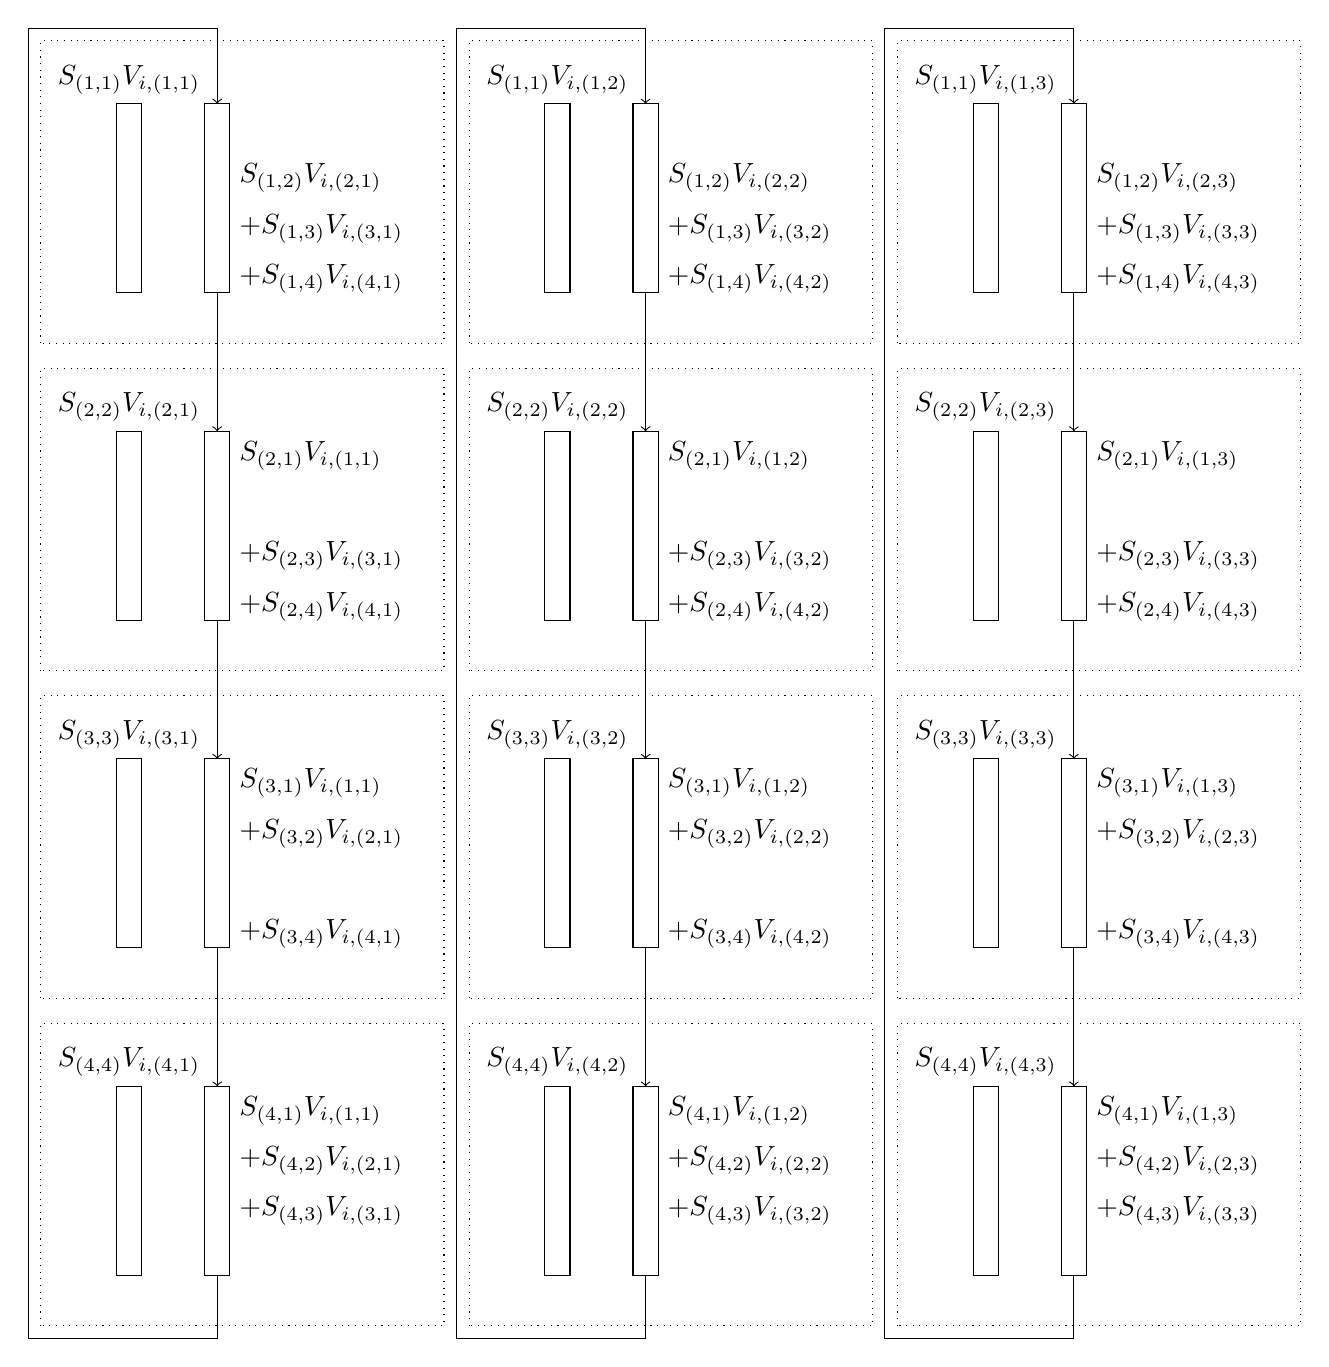
\begin{tikzpicture}[scale=16]
		% решетка процессов
		\draw [dotted] ( 0.00, 0.00 ) rectangle ( 0.32, 0.24 );
		\draw [dotted] ( 0.34, 0.00 ) rectangle ( 0.66, 0.24 );
		\draw [dotted] ( 0.68, 0.00 ) rectangle ( 1.00, 0.24 );
		\draw [dotted] ( 0.00, 0.26 ) rectangle ( 0.32, 0.50 );
		\draw [dotted] ( 0.34, 0.26 ) rectangle ( 0.66, 0.50 );
		\draw [dotted] ( 0.68, 0.26 ) rectangle ( 1.00, 0.50 );
		\draw [dotted] ( 0.00, 0.52 ) rectangle ( 0.32, 0.76 );
		\draw [dotted] ( 0.34, 0.52 ) rectangle ( 0.66, 0.76 );
		\draw [dotted] ( 0.68, 0.52 ) rectangle ( 1.00, 0.76 );
		\draw [dotted] ( 0.00, 0.78 ) rectangle ( 0.32, 1.02 );
		\draw [dotted] ( 0.34, 0.78 ) rectangle ( 0.66, 1.02 );
		\draw [dotted] ( 0.68, 0.78 ) rectangle ( 1.00, 1.02 );

		% процесс ( 1, 1 )
		\draw ( 0.06, 0.82 ) rectangle ( 0.08, 0.97 ) node [above] at ( 0.07, 0.97 ) {$S_{(1,1)} V_{i,(1,1)}$};
		\draw ( 0.13, 0.82 ) rectangle ( 0.15, 0.97 );
		\node [below right] at ( 0.15, 0.93 ) {$S_{(1,2)} V_{i,(2,1)}$};
		\node [below right] at ( 0.15, 0.89 ) {$+ S_{(1,3)} V_{i,(3,1)}$};
 		\node [below right] at ( 0.15, 0.85 ) {$+ S_{(1,4)} V_{i,(4,1)}$};
		\draw [->] ( 0.14, 0.82 ) -- ( 0.14, 0.71 );

		% процесс ( 1, 2 )
		\draw ( 0.40, 0.82 ) rectangle ( 0.42, 0.97 ) node [above] at ( 0.41, 0.97 ) {$S_{(1,1)} V_{i,(1,2)}$};
		\draw ( 0.47, 0.82 ) rectangle ( 0.49, 0.97 );
		\node [below right] at ( 0.49, 0.93 ) {$S_{(1,2)} V_{i,(2,2)}$};
		\node [below right] at ( 0.49, 0.89 ) {$+ S_{(1,3)} V_{i,(3,2)}$};
 		\node [below right] at ( 0.49, 0.85 ) {$+ S_{(1,4)} V_{i,(4,2)}$};
		\draw [->] ( 0.48, 0.82 ) -- ( 0.48, 0.71 );

		% процесс ( 1, 3 )
		\draw ( 0.74, 0.82 ) rectangle ( 0.76, 0.97 ) node [above] at ( 0.75, 0.97 ) {$S_{(1,1)} V_{i,(1,3)}$};
		\draw ( 0.81, 0.82 ) rectangle ( 0.83, 0.97 );
		\node [below right] at ( 0.83, 0.93 ) {$S_{(1,2)} V_{i,(2,3)}$};
		\node [below right] at ( 0.83, 0.89 ) {$+ S_{(1,3)} V_{i,(3,3)}$};
 		\node [below right] at ( 0.83, 0.85 ) {$+ S_{(1,4)} V_{i,(4,3)}$};
		\draw [->] ( 0.82, 0.82 ) -- ( 0.82, 0.71 );

		% процесс ( 2, 1 )
		\draw ( 0.06, 0.56 ) rectangle ( 0.08, 0.71 ) node [above] at ( 0.07, 0.71 ) {$S_{(2,2)} V_{i,(2,1)}$};
		\draw ( 0.13, 0.56 ) rectangle ( 0.15, 0.71 );
 		\node [below right] at ( 0.15, 0.71 ) {$S_{(2,1)} V_{i,(1,1)}$};
		\node [below right] at ( 0.15, 0.63 ) {$+ S_{(2,3)} V_{i,(3,1)}$};
 		\node [below right] at ( 0.15, 0.59 ) {$+ S_{(2,4)} V_{i,(4,1)}$};
		\draw [->] ( 0.14, 0.56 ) -- ( 0.14, 0.45 );

		% процесс ( 2, 2 )
		\draw ( 0.40, 0.56 ) rectangle ( 0.42, 0.71 ) node [above] at ( 0.41, 0.71 ) {$S_{(2,2)} V_{i,(2,2)}$};
		\draw ( 0.47, 0.56 ) rectangle ( 0.49, 0.71 );
 		\node [below right] at ( 0.49, 0.71 ) {$S_{(2,1)} V_{i,(1,2)}$};
		\node [below right] at ( 0.49, 0.63 ) {$+ S_{(2,3)} V_{i,(3,2)}$};
		\node [below right] at ( 0.49, 0.59 ) {$+ S_{(2,4)} V_{i,(4,2)}$};
		\draw [->] ( 0.48, 0.56 ) -- ( 0.48, 0.45 );

		% процесс ( 2, 3 )
		\draw ( 0.74, 0.56 ) rectangle ( 0.76, 0.71 ) node [above] at ( 0.75, 0.71 ) {$S_{(2,2)} V_{i,(2,3)}$};
		\draw ( 0.81, 0.56 ) rectangle ( 0.83, 0.71 );
 		\node [below right] at ( 0.83, 0.71 ) {$S_{(2,1)} V_{i,(1,3)}$};
		\node [below right] at ( 0.83, 0.63 ) {$+ S_{(2,3)} V_{i,(3,3)}$};
		\node [below right] at ( 0.83, 0.59 ) {$+ S_{(2,4)} V_{i,(4,3)}$};
		\draw [->] ( 0.82, 0.56 ) -- ( 0.82, 0.45 );

		% процесс ( 3, 1 )
		\draw ( 0.06, 0.30 ) rectangle ( 0.08, 0.45 ) node [above] at ( 0.07, 0.45 ) {$S_{(3,3)} V_{i,(3,1)}$};
		\draw ( 0.13, 0.30 ) rectangle ( 0.15, 0.45 );
		\node [below right] at ( 0.15, 0.45 ) {$S_{(3,1)} V_{i,(1,1)}$};
 		\node [below right] at ( 0.15, 0.41 ) {$+ S_{(3,2)} V_{i,(2,1)}$};
		\node [below right] at ( 0.15, 0.33 ) {$+ S_{(3,4)} V_{i,(4,1)}$};
		\draw [->] ( 0.14, 0.30 ) -- ( 0.14, 0.19 );

		% процесс ( 3, 2 )
		\draw ( 0.40, 0.30 ) rectangle ( 0.42, 0.45 ) node [above] at ( 0.41, 0.45 ) {$S_{(3,3)} V_{i,(3,2)}$};
		\draw ( 0.47, 0.30 ) rectangle ( 0.49, 0.45 );
		\node [below right] at ( 0.49, 0.45 ) {$S_{(3,1)} V_{i,(1,2)}$};
 		\node [below right] at ( 0.49, 0.41 ) {$+ S_{(3,2)} V_{i,(2,2)}$};
		\node [below right] at ( 0.49, 0.33 ) {$+ S_{(3,4)} V_{i,(4,2)}$};
		\draw [->] ( 0.48, 0.30 ) -- ( 0.48, 0.19 );

		% процесс ( 3, 3 )
		\draw ( 0.74, 0.30 ) rectangle ( 0.76, 0.45 ) node [above] at ( 0.75, 0.45 ) {$S_{(3,3)} V_{i,(3,3)}$};
		\draw ( 0.81, 0.30 ) rectangle ( 0.83, 0.45 );
		\node [below right] at ( 0.83, 0.45 ) {$S_{(3,1)} V_{i,(1,3)}$};
 		\node [below right] at ( 0.83, 0.41 ) {$+ S_{(3,2)} V_{i,(2,3)}$};
		\node [below right] at ( 0.83, 0.33 ) {$+ S_{(3,4)} V_{i,(4,3)}$};
		\draw [->] ( 0.82, 0.30 ) -- ( 0.82, 0.19 );

		% процесс ( 4, 1 )
		\draw ( 0.06, 0.04 ) rectangle ( 0.08, 0.19 ) node [above] at ( 0.07, 0.19 ) {$S_{(4,4)} V_{i,(4,1)}$};
		\draw ( 0.13, 0.04 ) rectangle ( 0.15, 0.19 );
		\node [below right] at ( 0.15, 0.19 ) {$S_{(4,1)} V_{i,(1,1)}$};
		\node [below right] at ( 0.15, 0.15 ) {$+ S_{(4,2)} V_{i,(2,1)}$};
 		\node [below right] at ( 0.15, 0.11 ) {$+ S_{(4,3)} V_{i,(3,1)}$};
		\draw [->] ( 0.14, 0.04 ) -- ( 0.14, -0.01 ) -- ( -0.01, -0.01 ) -- ( -0.01, 1.03 ) -- ( 0.14, 1.03 ) -- ( 0.14, 0.97 );

		% процесс ( 4, 2 )
		\draw ( 0.40, 0.04 ) rectangle ( 0.42, 0.19 ) node [above] at ( 0.41, 0.19 ) {$S_{(4,4)} V_{i,(4,2)}$};
		\draw ( 0.47, 0.04 ) rectangle ( 0.49, 0.19 );
		\node [below right] at ( 0.49, 0.19 ) {$S_{(4,1)} V_{i,(1,2)}$};
		\node [below right] at ( 0.49, 0.15 ) {$+ S_{(4,2)} V_{i,(2,2)}$};
 		\node [below right] at ( 0.49, 0.11 ) {$+ S_{(4,3)} V_{i,(3,2)}$};
		\draw [->] ( 0.48, 0.04 ) -- ( 0.48, -0.01 ) -- ( 0.33, -0.01 ) -- ( 0.33, 1.03 ) -- ( 0.48, 1.03 ) -- ( 0.48, 0.97 );

		% процесс ( 4, 3 )
		\draw ( 0.74, 0.04 ) rectangle ( 0.76, 0.19 ) node [above] at ( 0.75, 0.19 ) {$S_{(4,4)} V_{i,(4,3)}$};
		\draw ( 0.81, 0.04 ) rectangle ( 0.83, 0.19 );
		\node [below right] at ( 0.83, 0.19 ) {$S_{(4,1)} V_{i,(1,3)}$};
		\node [below right] at ( 0.83, 0.15 ) {$+ S_{(4,2)} V_{i,(2,3)}$};
 		\node [below right] at ( 0.83, 0.11 ) {$+ S_{(4,3)} V_{i,(3,3)}$};
		\draw [->] ( 0.82, 0.04 ) -- ( 0.82, -0.01 ) -- ( 0.67, -0.01 ) -- ( 0.67, 1.03 ) -- ( 0.82, 1.03 ) -- ( 0.82, 0.97 );
	\end{tikzpicture}
	\caption{Вычисление $V_i^{(S)} = S V_i$: шаг 4а}
	\label{figure:csmi:S_V_step_4a}
\end{figure}

\begin{figure}
	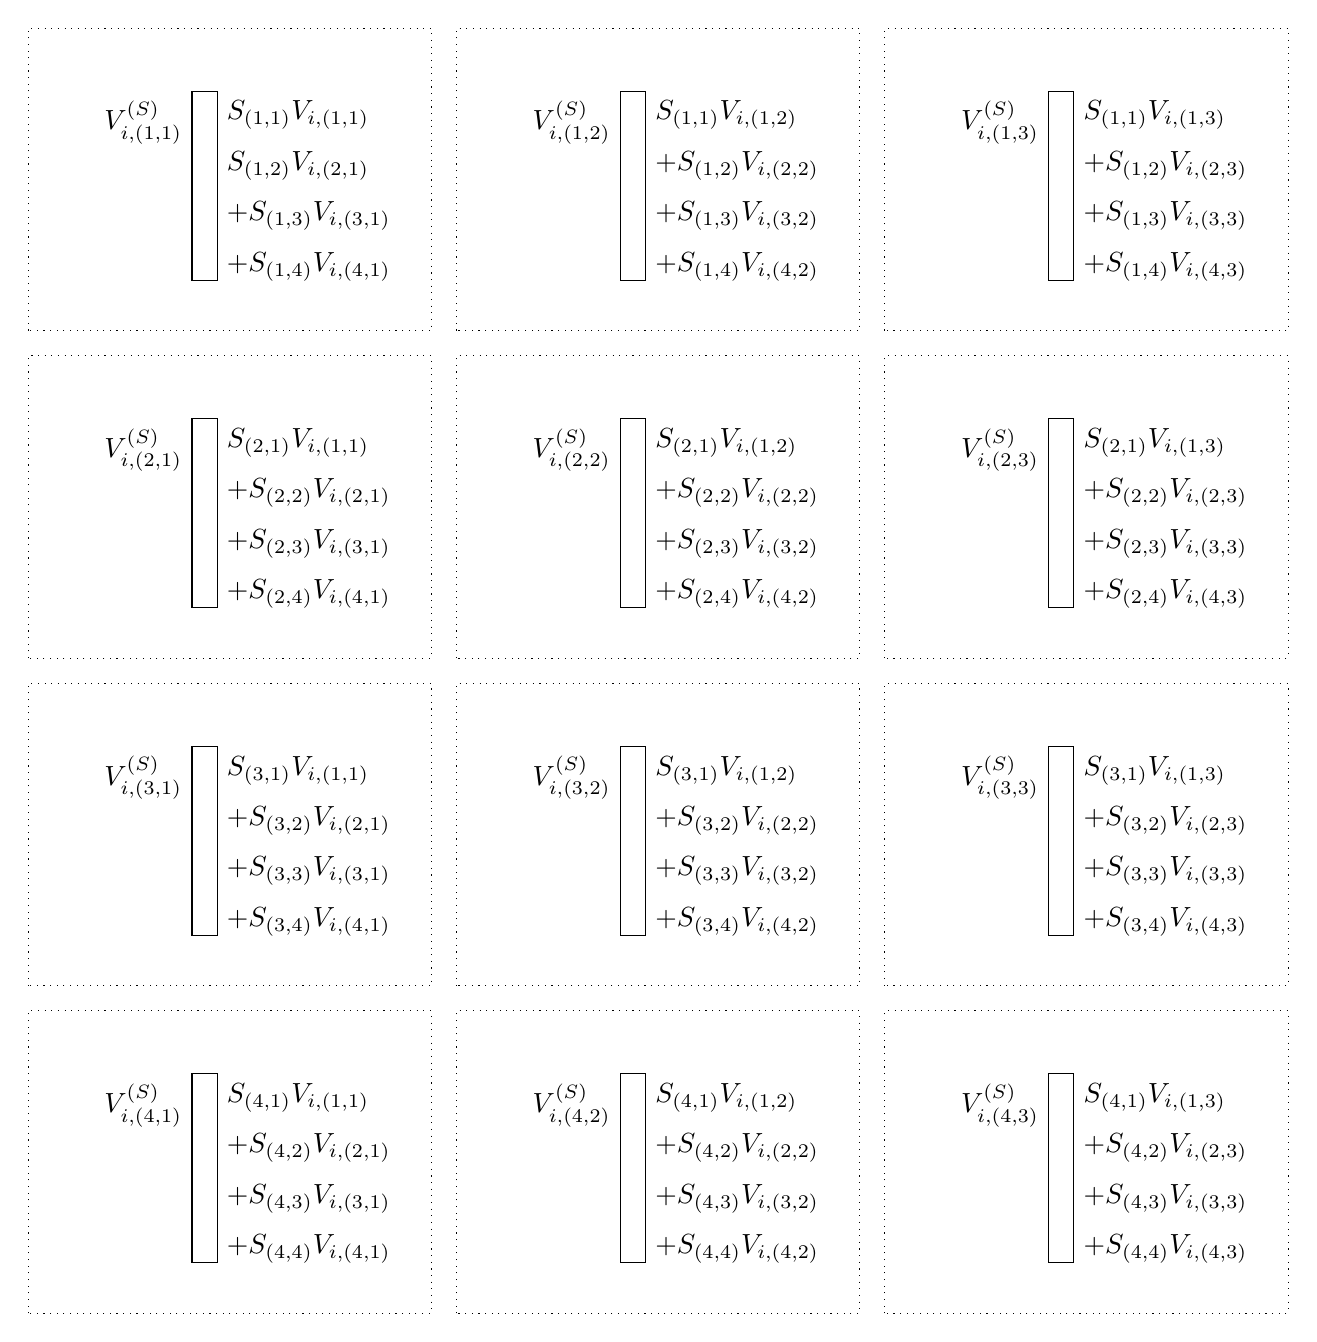
\begin{tikzpicture}[scale=16]
		% решетка процессов
		\draw [dotted] ( 0.00, 0.00 ) rectangle ( 0.32, 0.24 );
		\draw [dotted] ( 0.34, 0.00 ) rectangle ( 0.66, 0.24 );
		\draw [dotted] ( 0.68, 0.00 ) rectangle ( 1.00, 0.24 );
		\draw [dotted] ( 0.00, 0.26 ) rectangle ( 0.32, 0.50 );
		\draw [dotted] ( 0.34, 0.26 ) rectangle ( 0.66, 0.50 );
		\draw [dotted] ( 0.68, 0.26 ) rectangle ( 1.00, 0.50 );
		\draw [dotted] ( 0.00, 0.52 ) rectangle ( 0.32, 0.76 );
		\draw [dotted] ( 0.34, 0.52 ) rectangle ( 0.66, 0.76 );
		\draw [dotted] ( 0.68, 0.52 ) rectangle ( 1.00, 0.76 );
		\draw [dotted] ( 0.00, 0.78 ) rectangle ( 0.32, 1.02 );
		\draw [dotted] ( 0.34, 0.78 ) rectangle ( 0.66, 1.02 );
		\draw [dotted] ( 0.68, 0.78 ) rectangle ( 1.00, 1.02 );

		% процесс ( 1, 1 )
		\draw ( 0.13, 0.82 ) rectangle ( 0.15, 0.97 );
		\node [below left] at ( 0.13, 0.97 ) {$V_{i,(1,1)}^{(S)}$};
		\node [below right] at ( 0.15, 0.97 ) {$S_{(1,1)} V_{i,(1,1)}$};
		\node [below right] at ( 0.15, 0.93 ) {$S_{(1,2)} V_{i,(2,1)}$};
		\node [below right] at ( 0.15, 0.89 ) {$+ S_{(1,3)} V_{i,(3,1)}$};
 		\node [below right] at ( 0.15, 0.85 ) {$+ S_{(1,4)} V_{i,(4,1)}$};

		% процесс ( 1, 2 )
		\draw ( 0.47, 0.82 ) rectangle ( 0.49, 0.97 );
		\node [below left] at ( 0.47, 0.97 ) {$V_{i,(1,2)}^{(S)}$};
		\node [below right] at ( 0.49, 0.97 ) {$S_{(1,1)} V_{i,(1,2)}$};
		\node [below right] at ( 0.49, 0.93 ) {$+ S_{(1,2)} V_{i,(2,2)}$};
		\node [below right] at ( 0.49, 0.89 ) {$+ S_{(1,3)} V_{i,(3,2)}$};
 		\node [below right] at ( 0.49, 0.85 ) {$+ S_{(1,4)} V_{i,(4,2)}$};

		% процесс ( 1, 3 )
		\draw ( 0.81, 0.82 ) rectangle ( 0.83, 0.97 );
		\node [below left] at ( 0.81, 0.97 ) {$V_{i,(1,3)}^{(S)}$};
		\node [below right] at ( 0.83, 0.97 ) {$S_{(1,1)} V_{i,(1,3)}$};
		\node [below right] at ( 0.83, 0.93 ) {$+ S_{(1,2)} V_{i,(2,3)}$};
		\node [below right] at ( 0.83, 0.89 ) {$+ S_{(1,3)} V_{i,(3,3)}$};
 		\node [below right] at ( 0.83, 0.85 ) {$+ S_{(1,4)} V_{i,(4,3)}$};

		% процесс ( 2, 1 )
		\draw ( 0.13, 0.56 ) rectangle ( 0.15, 0.71 );
		\node [below left] at ( 0.13, 0.71 ) {$V_{i,(2,1)}^{(S)}$};
 		\node [below right] at ( 0.15, 0.71 ) {$S_{(2,1)} V_{i,(1,1)}$};
		\node [below right] at ( 0.15, 0.67 ) {$+ S_{(2,2)} V_{i,(2,1)}$};
		\node [below right] at ( 0.15, 0.63 ) {$+ S_{(2,3)} V_{i,(3,1)}$};
 		\node [below right] at ( 0.15, 0.59 ) {$+ S_{(2,4)} V_{i,(4,1)}$};

		% процесс ( 2, 2 )
		\draw ( 0.47, 0.56 ) rectangle ( 0.49, 0.71 );
		\node [below left] at ( 0.47, 0.71 ) {$V_{i,(2,2)}^{(S)}$};
		\node [below right] at ( 0.49, 0.71 ) {$S_{(2,1)} V_{i,(1,2)}$};
		\node [below right] at ( 0.49, 0.67 ) {$+ S_{(2,2)} V_{i,(2,2)}$};
		\node [below right] at ( 0.49, 0.63 ) {$+ S_{(2,3)} V_{i,(3,2)}$};
		\node [below right] at ( 0.49, 0.59 ) {$+ S_{(2,4)} V_{i,(4,2)}$};

		% процесс ( 2, 3 )
		\draw ( 0.81, 0.56 ) rectangle ( 0.83, 0.71 );
		\node [below left] at ( 0.81, 0.71 ) {$V_{i,(2,3)}^{(S)}$};
 		\node [below right] at ( 0.83, 0.71 ) {$S_{(2,1)} V_{i,(1,3)}$};
		\node [below right] at ( 0.83, 0.67 ) {$+ S_{(2,2)} V_{i,(2,3)}$};
		\node [below right] at ( 0.83, 0.63 ) {$+ S_{(2,3)} V_{i,(3,3)}$};
		\node [below right] at ( 0.83, 0.59 ) {$+ S_{(2,4)} V_{i,(4,3)}$};

		% процесс ( 3, 1 )
		\draw ( 0.13, 0.30 ) rectangle ( 0.15, 0.45 );
		\node [below left] at ( 0.13, 0.45 ) {$V_{i,(3,1)}^{(S)}$};
		\node [below right] at ( 0.15, 0.45 ) {$S_{(3,1)} V_{i,(1,1)}$};
 		\node [below right] at ( 0.15, 0.41 ) {$+ S_{(3,2)} V_{i,(2,1)}$};
		\node [below right] at ( 0.15, 0.37 ) {$+ S_{(3,3)} V_{i,(3,1)}$};
		\node [below right] at ( 0.15, 0.33 ) {$+ S_{(3,4)} V_{i,(4,1)}$};

		% процесс ( 3, 2 )
		\draw ( 0.47, 0.30 ) rectangle ( 0.49, 0.45 );
		\node [below left] at ( 0.47, 0.45 ) {$V_{i,(3,2)}^{(S)}$};
		\node [below right] at ( 0.49, 0.45 ) {$S_{(3,1)} V_{i,(1,2)}$};
 		\node [below right] at ( 0.49, 0.41 ) {$+ S_{(3,2)} V_{i,(2,2)}$};
		\node [below right] at ( 0.49, 0.37 ) {$+ S_{(3,3)} V_{i,(3,2)}$};
		\node [below right] at ( 0.49, 0.33 ) {$+ S_{(3,4)} V_{i,(4,2)}$};

		% процесс ( 3, 3 )
		\draw ( 0.81, 0.30 ) rectangle ( 0.83, 0.45 );
		\node [below left] at ( 0.81, 0.45 ) {$V_{i,(3,3)}^{(S)}$};
		\node [below right] at ( 0.83, 0.45 ) {$S_{(3,1)} V_{i,(1,3)}$};
 		\node [below right] at ( 0.83, 0.41 ) {$+ S_{(3,2)} V_{i,(2,3)}$};
		\node [below right] at ( 0.83, 0.37 ) {$+ S_{(3,3)} V_{i,(3,3)}$};
		\node [below right] at ( 0.83, 0.33 ) {$+ S_{(3,4)} V_{i,(4,3)}$};

		% процесс ( 4, 1 )
		\draw ( 0.13, 0.04 ) rectangle ( 0.15, 0.19 );
		\node [below left] at ( 0.13, 0.19 ) {$V_{i,(4,1)}^{(S)}$};
		\node [below right] at ( 0.15, 0.19 ) {$S_{(4,1)} V_{i,(1,1)}$};
		\node [below right] at ( 0.15, 0.15 ) {$+ S_{(4,2)} V_{i,(2,1)}$};
 		\node [below right] at ( 0.15, 0.11 ) {$+ S_{(4,3)} V_{i,(3,1)}$};
 		\node [below right] at ( 0.15, 0.07 ) {$+ S_{(4,4)} V_{i,(4,1)}$};

		% процесс ( 4, 2 )
		\draw ( 0.47, 0.04 ) rectangle ( 0.49, 0.19 );
		\node [below left] at ( 0.47, 0.19 ) {$V_{i,(4,2)}^{(S)}$};
		\node [below right] at ( 0.49, 0.19 ) {$S_{(4,1)} V_{i,(1,2)}$};
		\node [below right] at ( 0.49, 0.15 ) {$+ S_{(4,2)} V_{i,(2,2)}$};
 		\node [below right] at ( 0.49, 0.11 ) {$+ S_{(4,3)} V_{i,(3,2)}$};
 		\node [below right] at ( 0.49, 0.07 ) {$+ S_{(4,4)} V_{i,(4,2)}$};

		% процесс ( 4, 3 )
		\draw ( 0.81, 0.04 ) rectangle ( 0.83, 0.19 );
		\node [below left] at ( 0.81, 0.19 ) {$V_{i,(4,3)}^{(S)}$};
		\node [below right] at ( 0.83, 0.19 ) {$S_{(4,1)} V_{i,(1,3)}$};
		\node [below right] at ( 0.83, 0.15 ) {$+ S_{(4,2)} V_{i,(2,3)}$};
 		\node [below right] at ( 0.83, 0.11 ) {$+ S_{(4,3)} V_{i,(3,3)}$};
 		\node [below right] at ( 0.83, 0.07 ) {$+ S_{(4,4)} V_{i,(4,3)}$};
	\end{tikzpicture}
	\caption{Вычисление $V_i^{(S)} = S V_i$: шаг 4б}
	\label{figure:csmi:S_V_step_4b}
\end{figure}

\subsection{Вычисление $V_i^{(SS)} = S^T S V_i$}

Вычисление блоков $V_i^{(SS)}$ производится аналогично вычислению блоков $V_i^{(S)}$ с той лишь разницей, что вместо блоков $S_{(j,k)}$ матрицы $S$ использовуются блоки
$S_{(j,k)}^T$ матрицы $S^T$.

\subsection{Вычисление $Q_i = V_i^T S^T S V_i$}

$$
	\begin{pmatrix}
		V_{i,(1,1)}^T & V_{i,(2,1)}^T & V_{i,(3,1)}^T & V_{i,(4,1)}^T \\
		V_{i,(1,2)}^T & V_{i,(2,2)}^T & V_{i,(3,2)}^T & V_{i,(4,2)}^T \\
		V_{i,(1,3)}^T & V_{i,(2,3)}^T & V_{i,(3,3)}^T & V_{i,(4,3)}^T
	\end{pmatrix}
	\times
	\begin{pmatrix}
		V_{i,(1,1)}^{(SS)} & V_{i,(1,2)}^{(SS)} & V_{i,(1,3)}^{(SS)} \\
		V_{i,(2,1)}^{(SS)} & V_{i,(2,2)}^{(SS)} & V_{i,(2,3)}^{(SS)} \\
		V_{i,(3,1)}^{(SS)} & V_{i,(3,2)}^{(SS)} & V_{i,(3,3)}^{(SS)} \\
		V_{i,(4,1)}^{(SS)} & V_{i,(4,2)}^{(SS)} & V_{i,(4,3)}^{(SS)}
	\end{pmatrix}
$$

$$
	\begin{pmatrix}
		V_{i,(1,1)}^T V_{i,(1,1)}^{(SS)} + V_{i,(2,1)}^T V_{i,(2,1)}^{(SS)} + V_{i,(3,1)}^T V_{i,(3,1)}^{(SS)} + V_{i,(4,1)}^T V_{i,(4,1)}^{(SS)}
	\end{pmatrix}
$$

\begin{figure}
	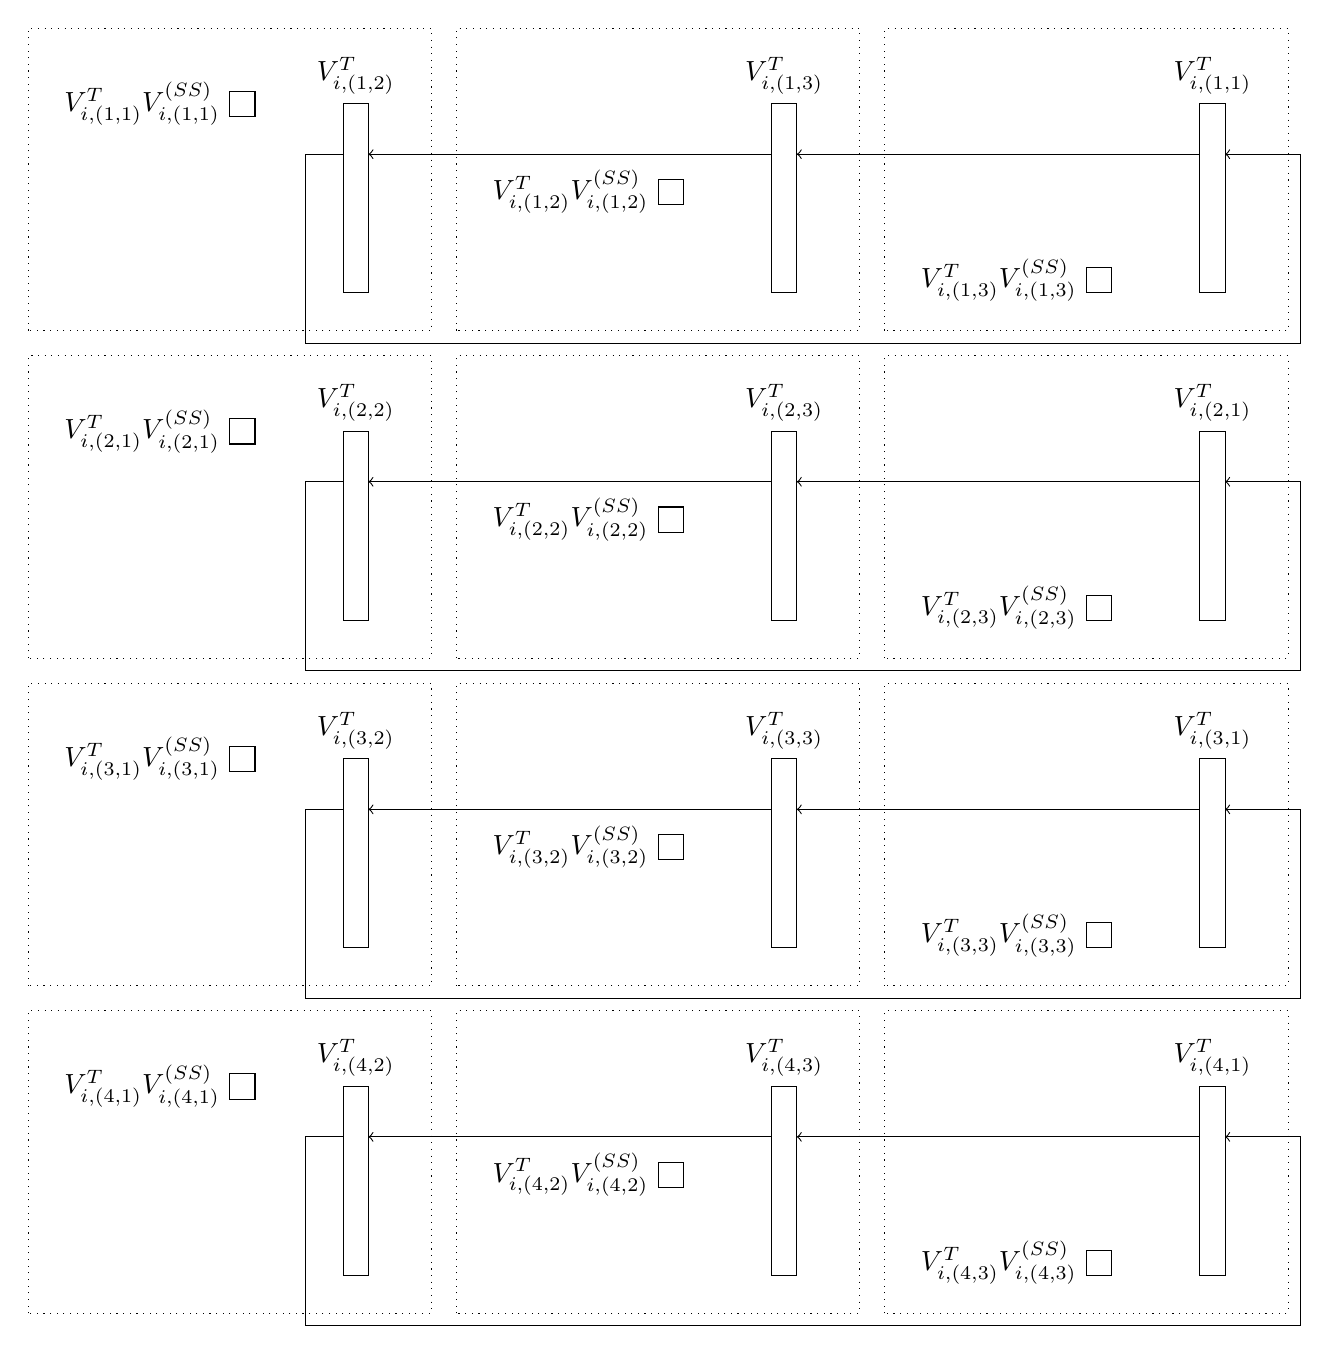
\begin{tikzpicture}[scale=16]
		% решетка процессов
		\draw [dotted] ( 0.00, 0.00 ) rectangle ( 0.32, 0.24 );
		\draw [dotted] ( 0.34, 0.00 ) rectangle ( 0.66, 0.24 );
		\draw [dotted] ( 0.68, 0.00 ) rectangle ( 1.00, 0.24 );
		\draw [dotted] ( 0.00, 0.26 ) rectangle ( 0.32, 0.50 );
		\draw [dotted] ( 0.34, 0.26 ) rectangle ( 0.66, 0.50 );
		\draw [dotted] ( 0.68, 0.26 ) rectangle ( 1.00, 0.50 );
		\draw [dotted] ( 0.00, 0.52 ) rectangle ( 0.32, 0.76 );
		\draw [dotted] ( 0.34, 0.52 ) rectangle ( 0.66, 0.76 );
		\draw [dotted] ( 0.68, 0.52 ) rectangle ( 1.00, 0.76 );
		\draw [dotted] ( 0.00, 0.78 ) rectangle ( 0.32, 1.02 );
		\draw [dotted] ( 0.34, 0.78 ) rectangle ( 0.66, 1.02 );
		\draw [dotted] ( 0.68, 0.78 ) rectangle ( 1.00, 1.02 );

		% процесс ( 1, 1 )
		\draw ( 0.16, 0.95 ) rectangle ( 0.18, 0.97 ) node [left] at ( 0.16, 0.96 ) {$V_{i,(1,1)}^T V_{i,(1,1)}^{(SS)}$};
		\draw ( 0.25, 0.81 ) rectangle ( 0.27, 0.96 ) node [above] at ( 0.26, 0.96 ) {$V_{i,(1,2)}^T$};
		\draw [->] ( 0.25, 0.92 ) -- ( 0.22, 0.92 ) -- ( 0.22, 0.77 ) -- ( 1.01, 0.77 ) -- ( 1.01, 0.92 ) -- ( 0.95, 0.92 ); 

		% процесс ( 1, 2 )
		\draw ( 0.50, 0.88 ) rectangle ( 0.52, 0.90 ) node [left] at ( 0.50, 0.89 ) {$V_{i,(1,2)}^T V_{i,(1,2)}^{(SS)}$};
		\draw ( 0.59, 0.81 ) rectangle ( 0.61, 0.96 ) node [above] at ( 0.60, 0.96 ) {$V_{i,(1,3)}^T$};
		\draw [->] ( 0.59, 0.92 ) -- ( 0.27, 0.92 ); 

		% процесс ( 1, 3 )
		\draw ( 0.84, 0.81 ) rectangle ( 0.86, 0.83 ) node [left] at ( 0.84, 0.82 ) {$V_{i,(1,3)}^T V_{i,(1,3)}^{(SS)}$};
		\draw ( 0.93, 0.81 ) rectangle ( 0.95, 0.96 ) node [above] at ( 0.94, 0.96 ) {$V_{i,(1,1)}^T$};
		\draw [->] ( 0.93, 0.92 ) -- ( 0.61, 0.92 ); 

		% процесс ( 2, 1 )
		\draw ( 0.16, 0.69 ) rectangle ( 0.18, 0.71 ) node [left] at ( 0.16, 0.70 ) {$V_{i,(2,1)}^T V_{i,(2,1)}^{(SS)}$};
		\draw ( 0.25, 0.55 ) rectangle ( 0.27, 0.70 ) node [above] at ( 0.26, 0.70 ) {$V_{i,(2,2)}^T$};
		\draw [->] ( 0.25, 0.66 ) -- ( 0.22, 0.66 ) -- ( 0.22, 0.51 ) -- ( 1.01, 0.51 ) -- ( 1.01, 0.66 ) -- ( 0.95, 0.66 ); 

		% процесс ( 2, 2 )
		\draw ( 0.50, 0.62 ) rectangle ( 0.52, 0.64 ) node [left] at ( 0.50, 0.63 ) {$V_{i,(2,2)}^T V_{i,(2,2)}^{(SS)}$};
		\draw ( 0.59, 0.55 ) rectangle ( 0.61, 0.70 ) node [above] at ( 0.60, 0.70 ) {$V_{i,(2,3)}^T$};
		\draw [->] ( 0.59, 0.66 ) -- ( 0.27, 0.66 ); 

		% процесс ( 2, 3 )
		\draw ( 0.84, 0.55 ) rectangle ( 0.86, 0.57 ) node [left] at ( 0.84, 0.56 ) {$V_{i,(2,3)}^T V_{i,(2,3)}^{(SS)}$};
		\draw ( 0.93, 0.55 ) rectangle ( 0.95, 0.70 ) node [above] at ( 0.94, 0.70 ) {$V_{i,(2,1)}^T$};
		\draw [->] ( 0.93, 0.66 ) -- ( 0.61, 0.66 ); 

		% процесс ( 3, 1 )
		\draw ( 0.16, 0.43 ) rectangle ( 0.18, 0.45 ) node [left] at ( 0.16, 0.44 ) {$V_{i,(3,1)}^T V_{i,(3,1)}^{(SS)}$};
		\draw ( 0.25, 0.29 ) rectangle ( 0.27, 0.44 ) node [above] at ( 0.26, 0.44 ) {$V_{i,(3,2)}^T$};
		\draw [->] ( 0.25, 0.40 ) -- ( 0.22, 0.40 ) -- ( 0.22, 0.25 ) -- ( 1.01, 0.25 ) -- ( 1.01, 0.40 ) -- ( 0.95, 0.40 ); 

		% процесс ( 3, 2 )
		\draw ( 0.50, 0.36 ) rectangle ( 0.52, 0.38 ) node [left] at ( 0.50, 0.37 ) {$V_{i,(3,2)}^T V_{i,(3,2)}^{(SS)}$};
		\draw ( 0.59, 0.29 ) rectangle ( 0.61, 0.44 ) node [above] at ( 0.60, 0.44 ) {$V_{i,(3,3)}^T$};
		\draw [->] ( 0.59, 0.40 ) -- ( 0.27, 0.40 ); 

		% процесс ( 3, 3 )
		\draw ( 0.84, 0.29 ) rectangle ( 0.86, 0.31 ) node [left] at ( 0.84, 0.30 ) {$V_{i,(3,3)}^T V_{i,(3,3)}^{(SS)}$};
		\draw ( 0.93, 0.29 ) rectangle ( 0.95, 0.44 ) node [above] at ( 0.94, 0.44 ) {$V_{i,(3,1)}^T$};
		\draw [->] ( 0.93, 0.40 ) -- ( 0.61, 0.40 ); 

		% процесс ( 4, 1 )
		\draw ( 0.16, 0.17 ) rectangle ( 0.18, 0.19 ) node [left] at ( 0.16, 0.18 ) {$V_{i,(4,1)}^T V_{i,(4,1)}^{(SS)}$};
		\draw ( 0.25, 0.03 ) rectangle ( 0.27, 0.18 ) node [above] at ( 0.26, 0.18 ) {$V_{i,(4,2)}^T$};
		\draw [->] ( 0.25, 0.14 ) -- ( 0.22, 0.14 ) -- ( 0.22, -0.01 ) -- ( 1.01, -0.01 ) -- ( 1.01, 0.14 ) -- ( 0.95, 0.14 ); 

		% процесс ( 4, 2 )
		\draw ( 0.50, 0.10 ) rectangle ( 0.52, 0.12 ) node [left] at ( 0.50, 0.11 ) {$V_{i,(4,2)}^T V_{i,(4,2)}^{(SS)}$};
		\draw ( 0.59, 0.03 ) rectangle ( 0.61, 0.18 ) node [above] at ( 0.60, 0.18 ) {$V_{i,(4,3)}^T$};
		\draw [->] ( 0.59, 0.14 ) -- ( 0.27, 0.14 ); 

		% процесс ( 4, 3 )
		\draw ( 0.84, 0.03 ) rectangle ( 0.86, 0.05 ) node [left] at ( 0.84, 0.04 ) {$V_{i,(4,3)}^T V_{i,(4,3)}^{(SS)}$};
		\draw ( 0.93, 0.03 ) rectangle ( 0.95, 0.18 ) node [above] at ( 0.94, 0.18 ) {$V_{i,(4,1)}^T$};
		\draw [->] ( 0.93, 0.14 ) -- ( 0.61, 0.14 ); 
	\end{tikzpicture}
	\caption{Вычисление $Q_i$: умножение со сдвигом, шаг 1}
\end{figure}

\begin{figure}
	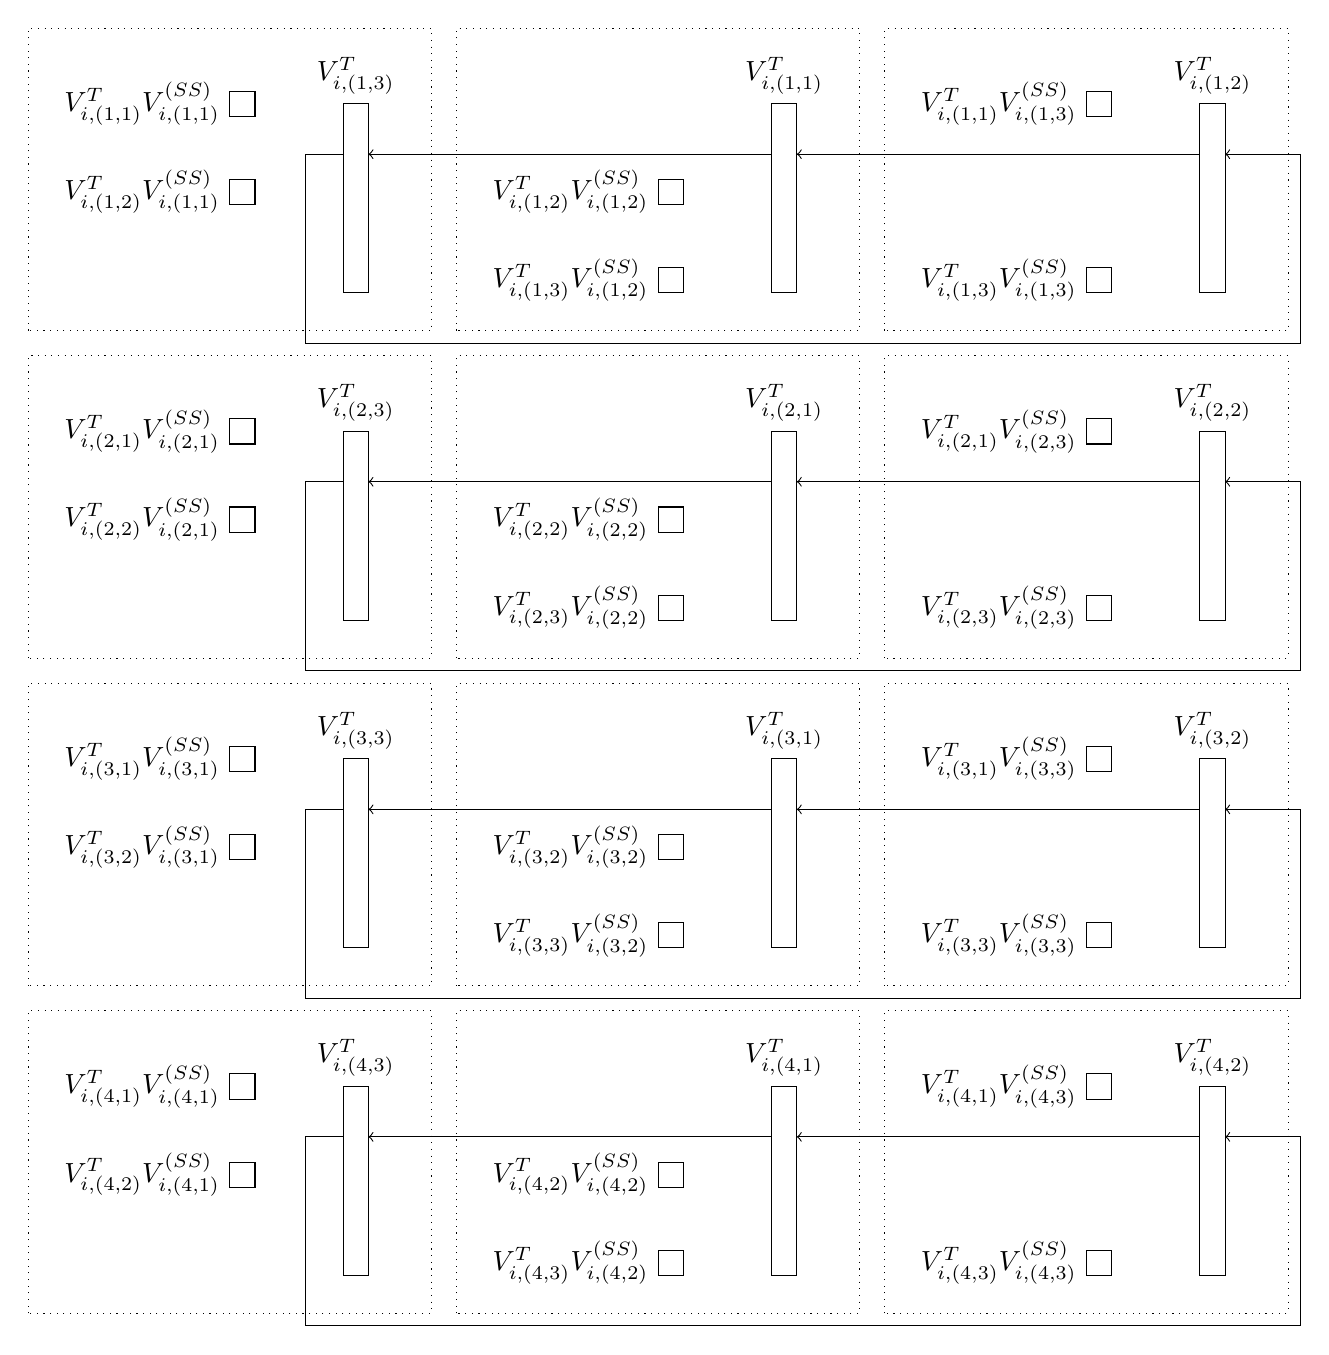
\begin{tikzpicture}[scale=16]
		% решетка процессов
		\draw [dotted] ( 0.00, 0.00 ) rectangle ( 0.32, 0.24 );
		\draw [dotted] ( 0.34, 0.00 ) rectangle ( 0.66, 0.24 );
		\draw [dotted] ( 0.68, 0.00 ) rectangle ( 1.00, 0.24 );
		\draw [dotted] ( 0.00, 0.26 ) rectangle ( 0.32, 0.50 );
		\draw [dotted] ( 0.34, 0.26 ) rectangle ( 0.66, 0.50 );
		\draw [dotted] ( 0.68, 0.26 ) rectangle ( 1.00, 0.50 );
		\draw [dotted] ( 0.00, 0.52 ) rectangle ( 0.32, 0.76 );
		\draw [dotted] ( 0.34, 0.52 ) rectangle ( 0.66, 0.76 );
		\draw [dotted] ( 0.68, 0.52 ) rectangle ( 1.00, 0.76 );
		\draw [dotted] ( 0.00, 0.78 ) rectangle ( 0.32, 1.02 );
		\draw [dotted] ( 0.34, 0.78 ) rectangle ( 0.66, 1.02 );
		\draw [dotted] ( 0.68, 0.78 ) rectangle ( 1.00, 1.02 );

		% процесс ( 1, 1 )
		\draw ( 0.16, 0.95 ) rectangle ( 0.18, 0.97 ) node [left] at ( 0.16, 0.96 ) {$V_{i,(1,1)}^T V_{i,(1,1)}^{(SS)}$};
		\draw ( 0.16, 0.88 ) rectangle ( 0.18, 0.90 ) node [left] at ( 0.16, 0.89 ) {$V_{i,(1,2)}^T V_{i,(1,1)}^{(SS)}$};
		\draw ( 0.25, 0.81 ) rectangle ( 0.27, 0.96 ) node [above] at ( 0.26, 0.96 ) {$V_{i,(1,3)}^T$};
		\draw [->] ( 0.25, 0.92 ) -- ( 0.22, 0.92 ) -- ( 0.22, 0.77 ) -- ( 1.01, 0.77 ) -- ( 1.01, 0.92 ) -- ( 0.95, 0.92 ); 

		% процесс ( 1, 2 )
		\draw ( 0.50, 0.88 ) rectangle ( 0.52, 0.90 ) node [left] at ( 0.50, 0.89 ) {$V_{i,(1,2)}^T V_{i,(1,2)}^{(SS)}$};
		\draw ( 0.50, 0.81 ) rectangle ( 0.52, 0.83 ) node [left] at ( 0.50, 0.82 ) {$V_{i,(1,3)}^T V_{i,(1,2)}^{(SS)}$};
		\draw ( 0.59, 0.81 ) rectangle ( 0.61, 0.96 ) node [above] at ( 0.60, 0.96 ) {$V_{i,(1,1)}^T$};
		\draw [->] ( 0.59, 0.92 ) -- ( 0.27, 0.92 ); 

		% процесс ( 1, 3 )
		\draw ( 0.84, 0.95 ) rectangle ( 0.86, 0.97 ) node [left] at ( 0.84, 0.96 ) {$V_{i,(1,1)}^T V_{i,(1,3)}^{(SS)}$};
		\draw ( 0.84, 0.81 ) rectangle ( 0.86, 0.83 ) node [left] at ( 0.84, 0.82 ) {$V_{i,(1,3)}^T V_{i,(1,3)}^{(SS)}$};
		\draw ( 0.93, 0.81 ) rectangle ( 0.95, 0.96 ) node [above] at ( 0.94, 0.96 ) {$V_{i,(1,2)}^T$};
		\draw [->] ( 0.93, 0.92 ) -- ( 0.61, 0.92 ); 

		% процесс ( 2, 1 )
		\draw ( 0.16, 0.69 ) rectangle ( 0.18, 0.71 ) node [left] at ( 0.16, 0.70 ) {$V_{i,(2,1)}^T V_{i,(2,1)}^{(SS)}$};
		\draw ( 0.16, 0.62 ) rectangle ( 0.18, 0.64 ) node [left] at ( 0.16, 0.63 ) {$V_{i,(2,2)}^T V_{i,(2,1)}^{(SS)}$};
		\draw ( 0.25, 0.55 ) rectangle ( 0.27, 0.70 ) node [above] at ( 0.26, 0.70 ) {$V_{i,(2,3)}^T$};
		\draw [->] ( 0.25, 0.66 ) -- ( 0.22, 0.66 ) -- ( 0.22, 0.51 ) -- ( 1.01, 0.51 ) -- ( 1.01, 0.66 ) -- ( 0.95, 0.66 ); 

		% процесс ( 2, 2 )
		\draw ( 0.50, 0.62 ) rectangle ( 0.52, 0.64 ) node [left] at ( 0.50, 0.63 ) {$V_{i,(2,2)}^T V_{i,(2,2)}^{(SS)}$};
		\draw ( 0.50, 0.55 ) rectangle ( 0.52, 0.57 ) node [left] at ( 0.50, 0.56 ) {$V_{i,(2,3)}^T V_{i,(2,2)}^{(SS)}$};
		\draw ( 0.59, 0.55 ) rectangle ( 0.61, 0.70 ) node [above] at ( 0.60, 0.70 ) {$V_{i,(2,1)}^T$};
		\draw [->] ( 0.59, 0.66 ) -- ( 0.27, 0.66 ); 

		% процесс ( 2, 3 )
		\draw ( 0.84, 0.69 ) rectangle ( 0.86, 0.71 ) node [left] at ( 0.84, 0.70 ) {$V_{i,(2,1)}^T V_{i,(2,3)}^{(SS)}$};
		\draw ( 0.84, 0.55 ) rectangle ( 0.86, 0.57 ) node [left] at ( 0.84, 0.56 ) {$V_{i,(2,3)}^T V_{i,(2,3)}^{(SS)}$};
		\draw ( 0.93, 0.55 ) rectangle ( 0.95, 0.70 ) node [above] at ( 0.94, 0.70 ) {$V_{i,(2,2)}^T$};
		\draw [->] ( 0.93, 0.66 ) -- ( 0.61, 0.66 ); 

		% процесс ( 3, 1 )
		\draw ( 0.16, 0.43 ) rectangle ( 0.18, 0.45 ) node [left] at ( 0.16, 0.44 ) {$V_{i,(3,1)}^T V_{i,(3,1)}^{(SS)}$};
		\draw ( 0.16, 0.36 ) rectangle ( 0.18, 0.38 ) node [left] at ( 0.16, 0.37 ) {$V_{i,(3,2)}^T V_{i,(3,1)}^{(SS)}$};
		\draw ( 0.25, 0.29 ) rectangle ( 0.27, 0.44 ) node [above] at ( 0.26, 0.44 ) {$V_{i,(3,3)}^T$};
		\draw [->] ( 0.25, 0.40 ) -- ( 0.22, 0.40 ) -- ( 0.22, 0.25 ) -- ( 1.01, 0.25 ) -- ( 1.01, 0.40 ) -- ( 0.95, 0.40 ); 

		% процесс ( 3, 2 )
		\draw ( 0.50, 0.36 ) rectangle ( 0.52, 0.38 ) node [left] at ( 0.50, 0.37 ) {$V_{i,(3,2)}^T V_{i,(3,2)}^{(SS)}$};
		\draw ( 0.50, 0.29 ) rectangle ( 0.52, 0.31 ) node [left] at ( 0.50, 0.30 ) {$V_{i,(3,3)}^T V_{i,(3,2)}^{(SS)}$};
		\draw ( 0.59, 0.29 ) rectangle ( 0.61, 0.44 ) node [above] at ( 0.60, 0.44 ) {$V_{i,(3,1)}^T$};
		\draw [->] ( 0.59, 0.40 ) -- ( 0.27, 0.40 ); 

		% процесс ( 3, 3 )
		\draw ( 0.84, 0.43 ) rectangle ( 0.86, 0.45 ) node [left] at ( 0.84, 0.44 ) {$V_{i,(3,1)}^T V_{i,(3,3)}^{(SS)}$};
		\draw ( 0.84, 0.29 ) rectangle ( 0.86, 0.31 ) node [left] at ( 0.84, 0.30 ) {$V_{i,(3,3)}^T V_{i,(3,3)}^{(SS)}$};
		\draw ( 0.93, 0.29 ) rectangle ( 0.95, 0.44 ) node [above] at ( 0.94, 0.44 ) {$V_{i,(3,2)}^T$};
		\draw [->] ( 0.93, 0.40 ) -- ( 0.61, 0.40 ); 

		% процесс ( 4, 1 )
		\draw ( 0.16, 0.17 ) rectangle ( 0.18, 0.19 ) node [left] at ( 0.16, 0.18 ) {$V_{i,(4,1)}^T V_{i,(4,1)}^{(SS)}$};
		\draw ( 0.16, 0.10 ) rectangle ( 0.18, 0.12 ) node [left] at ( 0.16, 0.11 ) {$V_{i,(4,2)}^T V_{i,(4,1)}^{(SS)}$};
		\draw ( 0.25, 0.03 ) rectangle ( 0.27, 0.18 ) node [above] at ( 0.26, 0.18 ) {$V_{i,(4,3)}^T$};
		\draw [->] ( 0.25, 0.14 ) -- ( 0.22, 0.14 ) -- ( 0.22, -0.01 ) -- ( 1.01, -0.01 ) -- ( 1.01, 0.14 ) -- ( 0.95, 0.14 ); 

		% процесс ( 4, 2 )
		\draw ( 0.50, 0.10 ) rectangle ( 0.52, 0.12 ) node [left] at ( 0.50, 0.11 ) {$V_{i,(4,2)}^T V_{i,(4,2)}^{(SS)}$};
		\draw ( 0.50, 0.03 ) rectangle ( 0.52, 0.05 ) node [left] at ( 0.50, 0.04 ) {$V_{i,(4,3)}^T V_{i,(4,2)}^{(SS)}$};
		\draw ( 0.59, 0.03 ) rectangle ( 0.61, 0.18 ) node [above] at ( 0.60, 0.18 ) {$V_{i,(4,1)}^T$};
		\draw [->] ( 0.59, 0.14 ) -- ( 0.27, 0.14 ); 

		% процесс ( 4, 3 )
		\draw ( 0.84, 0.17 ) rectangle ( 0.86, 0.19 ) node [left] at ( 0.84, 0.18 ) {$V_{i,(4,1)}^T V_{i,(4,3)}^{(SS)}$};
		\draw ( 0.84, 0.03 ) rectangle ( 0.86, 0.05 ) node [left] at ( 0.84, 0.04 ) {$V_{i,(4,3)}^T V_{i,(4,3)}^{(SS)}$};
		\draw ( 0.93, 0.03 ) rectangle ( 0.95, 0.18 ) node [above] at ( 0.94, 0.18 ) {$V_{i,(4,2)}^T$};
		\draw [->] ( 0.93, 0.14 ) -- ( 0.61, 0.14 ); 
	\end{tikzpicture}
	\caption{Вычисление $Q_i$: умножение со сдвигом, шаг 2}
\end{figure}

\begin{figure}
	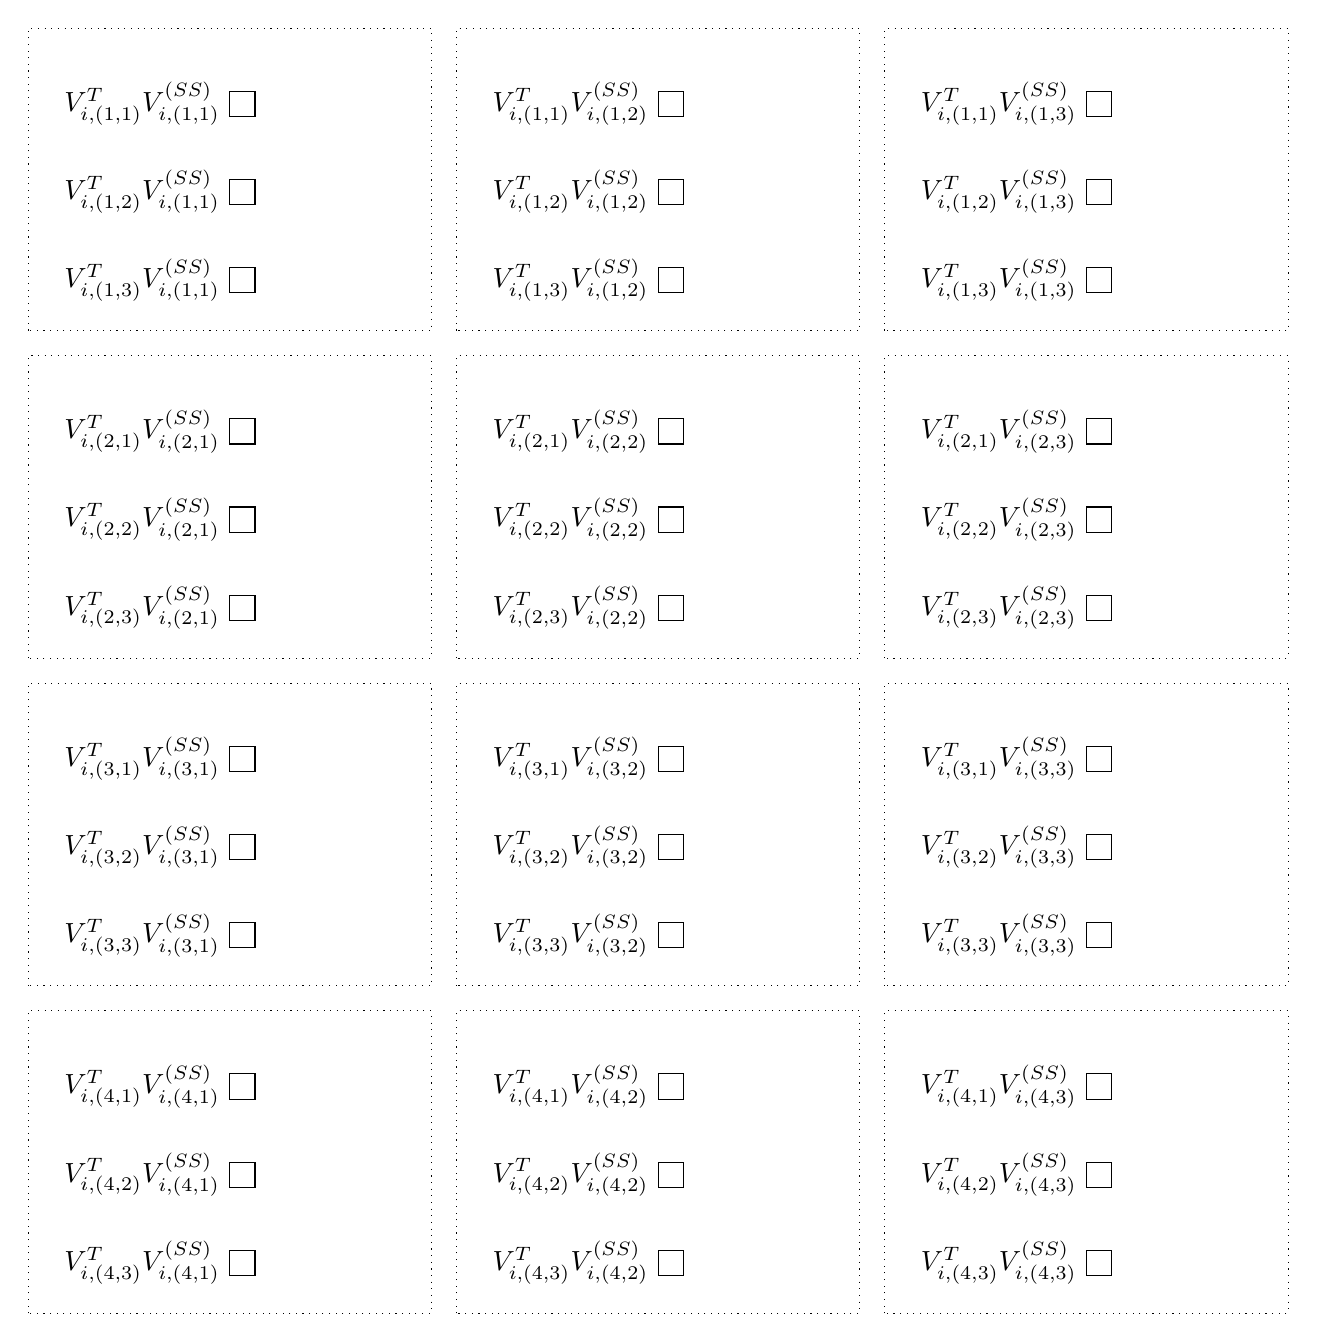
\begin{tikzpicture}[scale=16]
		% решетка процессов
		\draw [dotted] ( 0.00, 0.00 ) rectangle ( 0.32, 0.24 );
		\draw [dotted] ( 0.34, 0.00 ) rectangle ( 0.66, 0.24 );
		\draw [dotted] ( 0.68, 0.00 ) rectangle ( 1.00, 0.24 );
		\draw [dotted] ( 0.00, 0.26 ) rectangle ( 0.32, 0.50 );
		\draw [dotted] ( 0.34, 0.26 ) rectangle ( 0.66, 0.50 );
		\draw [dotted] ( 0.68, 0.26 ) rectangle ( 1.00, 0.50 );
		\draw [dotted] ( 0.00, 0.52 ) rectangle ( 0.32, 0.76 );
		\draw [dotted] ( 0.34, 0.52 ) rectangle ( 0.66, 0.76 );
		\draw [dotted] ( 0.68, 0.52 ) rectangle ( 1.00, 0.76 );
		\draw [dotted] ( 0.00, 0.78 ) rectangle ( 0.32, 1.02 );
		\draw [dotted] ( 0.34, 0.78 ) rectangle ( 0.66, 1.02 );
		\draw [dotted] ( 0.68, 0.78 ) rectangle ( 1.00, 1.02 );

		% процесс ( 1, 1 )
		\draw ( 0.16, 0.95 ) rectangle ( 0.18, 0.97 ) node [left] at ( 0.16, 0.96 ) {$V_{i,(1,1)}^T V_{i,(1,1)}^{(SS)}$};
		\draw ( 0.16, 0.88 ) rectangle ( 0.18, 0.90 ) node [left] at ( 0.16, 0.89 ) {$V_{i,(1,2)}^T V_{i,(1,1)}^{(SS)}$};
		\draw ( 0.16, 0.81 ) rectangle ( 0.18, 0.83 ) node [left] at ( 0.16, 0.82 ) {$V_{i,(1,3)}^T V_{i,(1,1)}^{(SS)}$};

		% процесс ( 1, 2 )
		\draw ( 0.50, 0.95 ) rectangle ( 0.52, 0.97 ) node [left] at ( 0.50, 0.96 ) {$V_{i,(1,1)}^T V_{i,(1,2)}^{(SS)}$};
		\draw ( 0.50, 0.88 ) rectangle ( 0.52, 0.90 ) node [left] at ( 0.50, 0.89 ) {$V_{i,(1,2)}^T V_{i,(1,2)}^{(SS)}$};
		\draw ( 0.50, 0.81 ) rectangle ( 0.52, 0.83 ) node [left] at ( 0.50, 0.82 ) {$V_{i,(1,3)}^T V_{i,(1,2)}^{(SS)}$};

		% процесс ( 1, 3 )
		\draw ( 0.84, 0.95 ) rectangle ( 0.86, 0.97 ) node [left] at ( 0.84, 0.96 ) {$V_{i,(1,1)}^T V_{i,(1,3)}^{(SS)}$};
		\draw ( 0.84, 0.88 ) rectangle ( 0.86, 0.90 ) node [left] at ( 0.84, 0.89 ) {$V_{i,(1,2)}^T V_{i,(1,3)}^{(SS)}$};
		\draw ( 0.84, 0.81 ) rectangle ( 0.86, 0.83 ) node [left] at ( 0.84, 0.82 ) {$V_{i,(1,3)}^T V_{i,(1,3)}^{(SS)}$};

		% процесс ( 2, 1 )
		\draw ( 0.16, 0.69 ) rectangle ( 0.18, 0.71 ) node [left] at ( 0.16, 0.70 ) {$V_{i,(2,1)}^T V_{i,(2,1)}^{(SS)}$};
		\draw ( 0.16, 0.62 ) rectangle ( 0.18, 0.64 ) node [left] at ( 0.16, 0.63 ) {$V_{i,(2,2)}^T V_{i,(2,1)}^{(SS)}$};
		\draw ( 0.16, 0.55 ) rectangle ( 0.18, 0.57 ) node [left] at ( 0.16, 0.56 ) {$V_{i,(2,3)}^T V_{i,(2,1)}^{(SS)}$};

		% процесс ( 2, 2 )
		\draw ( 0.50, 0.69 ) rectangle ( 0.52, 0.71 ) node [left] at ( 0.50, 0.70 ) {$V_{i,(2,1)}^T V_{i,(2,2)}^{(SS)}$};
		\draw ( 0.50, 0.62 ) rectangle ( 0.52, 0.64 ) node [left] at ( 0.50, 0.63 ) {$V_{i,(2,2)}^T V_{i,(2,2)}^{(SS)}$};
		\draw ( 0.50, 0.55 ) rectangle ( 0.52, 0.57 ) node [left] at ( 0.50, 0.56 ) {$V_{i,(2,3)}^T V_{i,(2,2)}^{(SS)}$};

		% процесс ( 2, 3 )
		\draw ( 0.84, 0.69 ) rectangle ( 0.86, 0.71 ) node [left] at ( 0.84, 0.70 ) {$V_{i,(2,1)}^T V_{i,(2,3)}^{(SS)}$};
		\draw ( 0.84, 0.62 ) rectangle ( 0.86, 0.64 ) node [left] at ( 0.84, 0.63 ) {$V_{i,(2,2)}^T V_{i,(2,3)}^{(SS)}$};
		\draw ( 0.84, 0.55 ) rectangle ( 0.86, 0.57 ) node [left] at ( 0.84, 0.56 ) {$V_{i,(2,3)}^T V_{i,(2,3)}^{(SS)}$};

		% процесс ( 3, 1 )
		\draw ( 0.16, 0.43 ) rectangle ( 0.18, 0.45 ) node [left] at ( 0.16, 0.44 ) {$V_{i,(3,1)}^T V_{i,(3,1)}^{(SS)}$};
		\draw ( 0.16, 0.36 ) rectangle ( 0.18, 0.38 ) node [left] at ( 0.16, 0.37 ) {$V_{i,(3,2)}^T V_{i,(3,1)}^{(SS)}$};
		\draw ( 0.16, 0.29 ) rectangle ( 0.18, 0.31 ) node [left] at ( 0.16, 0.30 ) {$V_{i,(3,3)}^T V_{i,(3,1)}^{(SS)}$};

		% процесс ( 3, 2 )
		\draw ( 0.50, 0.43 ) rectangle ( 0.52, 0.45 ) node [left] at ( 0.50, 0.44 ) {$V_{i,(3,1)}^T V_{i,(3,2)}^{(SS)}$};
		\draw ( 0.50, 0.36 ) rectangle ( 0.52, 0.38 ) node [left] at ( 0.50, 0.37 ) {$V_{i,(3,2)}^T V_{i,(3,2)}^{(SS)}$};
		\draw ( 0.50, 0.29 ) rectangle ( 0.52, 0.31 ) node [left] at ( 0.50, 0.30 ) {$V_{i,(3,3)}^T V_{i,(3,2)}^{(SS)}$};

		% процесс ( 3, 3 )
		\draw ( 0.84, 0.43 ) rectangle ( 0.86, 0.45 ) node [left] at ( 0.84, 0.44 ) {$V_{i,(3,1)}^T V_{i,(3,3)}^{(SS)}$};
		\draw ( 0.84, 0.36 ) rectangle ( 0.86, 0.38 ) node [left] at ( 0.84, 0.37 ) {$V_{i,(3,2)}^T V_{i,(3,3)}^{(SS)}$};
		\draw ( 0.84, 0.29 ) rectangle ( 0.86, 0.31 ) node [left] at ( 0.84, 0.30 ) {$V_{i,(3,3)}^T V_{i,(3,3)}^{(SS)}$};

		% процесс ( 4, 1 )
		\draw ( 0.16, 0.17 ) rectangle ( 0.18, 0.19 ) node [left] at ( 0.16, 0.18 ) {$V_{i,(4,1)}^T V_{i,(4,1)}^{(SS)}$};
		\draw ( 0.16, 0.10 ) rectangle ( 0.18, 0.12 ) node [left] at ( 0.16, 0.11 ) {$V_{i,(4,2)}^T V_{i,(4,1)}^{(SS)}$};
		\draw ( 0.16, 0.03 ) rectangle ( 0.18, 0.05 ) node [left] at ( 0.16, 0.04 ) {$V_{i,(4,3)}^T V_{i,(4,1)}^{(SS)}$};

		% процесс ( 4, 2 )
		\draw ( 0.50, 0.17 ) rectangle ( 0.52, 0.19 ) node [left] at ( 0.50, 0.18 ) {$V_{i,(4,1)}^T V_{i,(4,2)}^{(SS)}$};
		\draw ( 0.50, 0.10 ) rectangle ( 0.52, 0.12 ) node [left] at ( 0.50, 0.11 ) {$V_{i,(4,2)}^T V_{i,(4,2)}^{(SS)}$};
		\draw ( 0.50, 0.03 ) rectangle ( 0.52, 0.05 ) node [left] at ( 0.50, 0.04 ) {$V_{i,(4,3)}^T V_{i,(4,2)}^{(SS)}$};

		% процесс ( 4, 3 )
		\draw ( 0.84, 0.17 ) rectangle ( 0.86, 0.19 ) node [left] at ( 0.84, 0.18 ) {$V_{i,(4,1)}^T V_{i,(4,3)}^{(SS)}$};
		\draw ( 0.84, 0.10 ) rectangle ( 0.86, 0.12 ) node [left] at ( 0.84, 0.11 ) {$V_{i,(4,2)}^T V_{i,(4,3)}^{(SS)}$};
		\draw ( 0.84, 0.03 ) rectangle ( 0.86, 0.05 ) node [left] at ( 0.84, 0.04 ) {$V_{i,(4,3)}^T V_{i,(4,3)}^{(SS)}$};
	\end{tikzpicture}
	\caption{Вычисление $Q_i$: умножение со сдвигом, шаг 3}
\end{figure}

\begin{figure}
	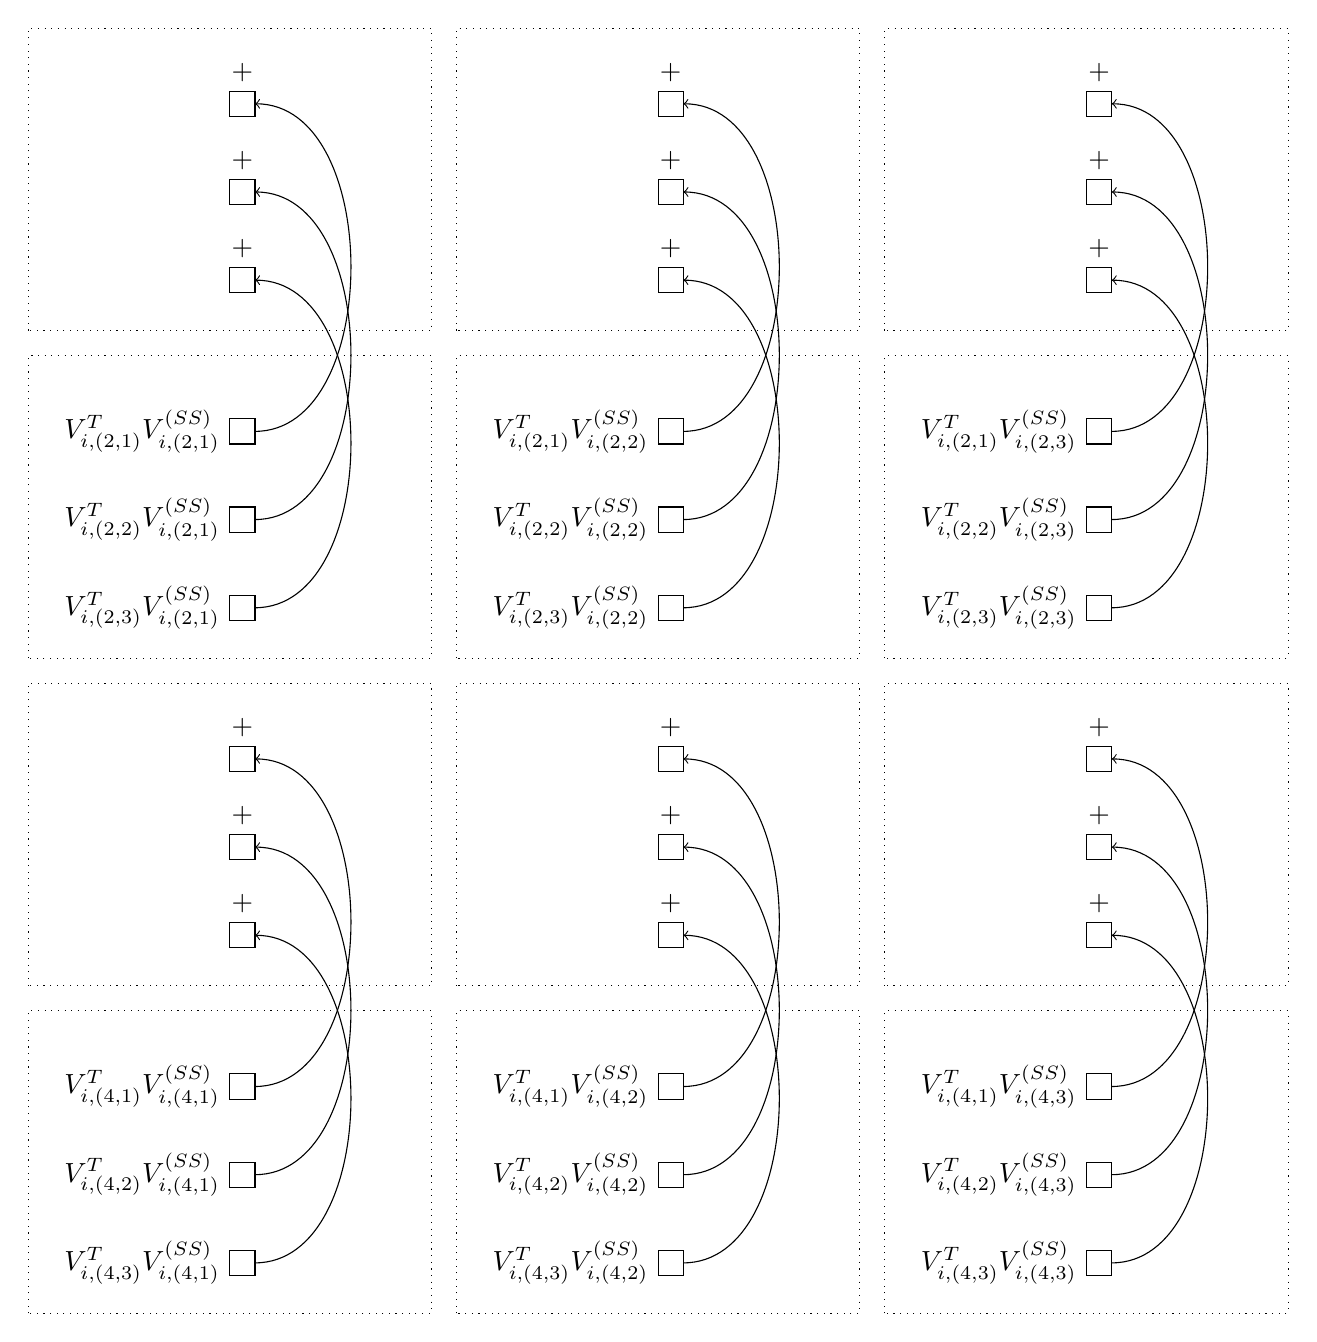
\begin{tikzpicture}[scale=16]
		% решетка процессов
		\draw [dotted] ( 0.00, 0.00 ) rectangle ( 0.32, 0.24 );
		\draw [dotted] ( 0.34, 0.00 ) rectangle ( 0.66, 0.24 );
		\draw [dotted] ( 0.68, 0.00 ) rectangle ( 1.00, 0.24 );
		\draw [dotted] ( 0.00, 0.26 ) rectangle ( 0.32, 0.50 );
		\draw [dotted] ( 0.34, 0.26 ) rectangle ( 0.66, 0.50 );
		\draw [dotted] ( 0.68, 0.26 ) rectangle ( 1.00, 0.50 );
		\draw [dotted] ( 0.00, 0.52 ) rectangle ( 0.32, 0.76 );
		\draw [dotted] ( 0.34, 0.52 ) rectangle ( 0.66, 0.76 );
		\draw [dotted] ( 0.68, 0.52 ) rectangle ( 1.00, 0.76 );
		\draw [dotted] ( 0.00, 0.78 ) rectangle ( 0.32, 1.02 );
		\draw [dotted] ( 0.34, 0.78 ) rectangle ( 0.66, 1.02 );
		\draw [dotted] ( 0.68, 0.78 ) rectangle ( 1.00, 1.02 );

		% процесс ( 1, 1 )
		\draw ( 0.16, 0.95 ) rectangle ( 0.18, 0.97 );
		\draw ( 0.16, 0.88 ) rectangle ( 0.18, 0.90 );
		\draw ( 0.16, 0.81 ) rectangle ( 0.18, 0.83 );
		\node [above] at ( 0.17, 0.97 ) {$+$};
		\node [above] at ( 0.17, 0.90 ) {$+$};
		\node [above] at ( 0.17, 0.83 ) {$+$};

		% процесс ( 1, 2 )
		\draw ( 0.50, 0.95 ) rectangle ( 0.52, 0.97 );
		\draw ( 0.50, 0.88 ) rectangle ( 0.52, 0.90 );
		\draw ( 0.50, 0.81 ) rectangle ( 0.52, 0.83 );
		\node [above] at ( 0.51, 0.97 ) {$+$};
		\node [above] at ( 0.51, 0.90 ) {$+$};
		\node [above] at ( 0.51, 0.83 ) {$+$};

		% процесс ( 1, 3 )
		\draw ( 0.84, 0.95 ) rectangle ( 0.86, 0.97 );
		\draw ( 0.84, 0.88 ) rectangle ( 0.86, 0.90 );
		\draw ( 0.84, 0.81 ) rectangle ( 0.86, 0.83 );
		\node [above] at ( 0.85, 0.97 ) {$+$};
		\node [above] at ( 0.85, 0.90 ) {$+$};
		\node [above] at ( 0.85, 0.83 ) {$+$};

		% процесс ( 2, 1 )
		\draw ( 0.16, 0.69 ) rectangle ( 0.18, 0.71 ) node [left] at ( 0.16, 0.70 ) {$V_{i,(2,1)}^T V_{i,(2,1)}^{(SS)}$};
		\draw ( 0.16, 0.62 ) rectangle ( 0.18, 0.64 ) node [left] at ( 0.16, 0.63 ) {$V_{i,(2,2)}^T V_{i,(2,1)}^{(SS)}$};
		\draw ( 0.16, 0.55 ) rectangle ( 0.18, 0.57 ) node [left] at ( 0.16, 0.56 ) {$V_{i,(2,3)}^T V_{i,(2,1)}^{(SS)}$};
		\draw [->] ( 0.18, 0.70 ) to [ out = 0, in = 0 ] ( 0.18, 0.96 );
		\draw [->] ( 0.18, 0.63 ) to [ out = 0, in = 0 ] ( 0.18, 0.89 );
		\draw [->] ( 0.18, 0.56 ) to [ out = 0, in = 0 ] ( 0.18, 0.82 );

		% процесс ( 2, 2 )
		\draw ( 0.50, 0.69 ) rectangle ( 0.52, 0.71 ) node [left] at ( 0.50, 0.70 ) {$V_{i,(2,1)}^T V_{i,(2,2)}^{(SS)}$};
		\draw ( 0.50, 0.62 ) rectangle ( 0.52, 0.64 ) node [left] at ( 0.50, 0.63 ) {$V_{i,(2,2)}^T V_{i,(2,2)}^{(SS)}$};
		\draw ( 0.50, 0.55 ) rectangle ( 0.52, 0.57 ) node [left] at ( 0.50, 0.56 ) {$V_{i,(2,3)}^T V_{i,(2,2)}^{(SS)}$};
		\draw [->] ( 0.52, 0.70 ) to [ out = 0, in = 0 ] ( 0.52, 0.96 );
		\draw [->] ( 0.52, 0.63 ) to [ out = 0, in = 0 ] ( 0.52, 0.89 );
		\draw [->] ( 0.52, 0.56 ) to [ out = 0, in = 0 ] ( 0.52, 0.82 );

		% процесс ( 2, 3 )
		\draw ( 0.84, 0.69 ) rectangle ( 0.86, 0.71 ) node [left] at ( 0.84, 0.70 ) {$V_{i,(2,1)}^T V_{i,(2,3)}^{(SS)}$};
		\draw ( 0.84, 0.62 ) rectangle ( 0.86, 0.64 ) node [left] at ( 0.84, 0.63 ) {$V_{i,(2,2)}^T V_{i,(2,3)}^{(SS)}$};
		\draw ( 0.84, 0.55 ) rectangle ( 0.86, 0.57 ) node [left] at ( 0.84, 0.56 ) {$V_{i,(2,3)}^T V_{i,(2,3)}^{(SS)}$};
		\draw [->] ( 0.86, 0.70 ) to [ out = 0, in = 0 ] ( 0.86, 0.96 );
		\draw [->] ( 0.86, 0.63 ) to [ out = 0, in = 0 ] ( 0.86, 0.89 );
		\draw [->] ( 0.86, 0.56 ) to [ out = 0, in = 0 ] ( 0.86, 0.82 );

		% процесс ( 3, 1 )
		\draw ( 0.16, 0.43 ) rectangle ( 0.18, 0.45 );
		\draw ( 0.16, 0.36 ) rectangle ( 0.18, 0.38 );
		\draw ( 0.16, 0.29 ) rectangle ( 0.18, 0.31 );
		\node [above] at ( 0.17, 0.45 ) {$+$};
		\node [above] at ( 0.17, 0.38 ) {$+$};
		\node [above] at ( 0.17, 0.31 ) {$+$};

		% процесс ( 3, 2 )
		\draw ( 0.50, 0.43 ) rectangle ( 0.52, 0.45 );
		\draw ( 0.50, 0.36 ) rectangle ( 0.52, 0.38 );
		\draw ( 0.50, 0.29 ) rectangle ( 0.52, 0.31 );
		\node [above] at ( 0.51, 0.45 ) {$+$};
		\node [above] at ( 0.51, 0.38 ) {$+$};
		\node [above] at ( 0.51, 0.31 ) {$+$};

		% процесс ( 3, 3 )
		\draw ( 0.84, 0.43 ) rectangle ( 0.86, 0.45 );
		\draw ( 0.84, 0.36 ) rectangle ( 0.86, 0.38 );
		\draw ( 0.84, 0.29 ) rectangle ( 0.86, 0.31 );
		\node [above] at ( 0.85, 0.45 ) {$+$};
		\node [above] at ( 0.85, 0.38 ) {$+$};
		\node [above] at ( 0.85, 0.31 ) {$+$};

		% процесс ( 4, 1 )
		\draw ( 0.16, 0.17 ) rectangle ( 0.18, 0.19 ) node [left] at ( 0.16, 0.18 ) {$V_{i,(4,1)}^T V_{i,(4,1)}^{(SS)}$};
		\draw ( 0.16, 0.10 ) rectangle ( 0.18, 0.12 ) node [left] at ( 0.16, 0.11 ) {$V_{i,(4,2)}^T V_{i,(4,1)}^{(SS)}$};
		\draw ( 0.16, 0.03 ) rectangle ( 0.18, 0.05 ) node [left] at ( 0.16, 0.04 ) {$V_{i,(4,3)}^T V_{i,(4,1)}^{(SS)}$};
		\draw [->] ( 0.18, 0.18 ) to [ out = 0, in = 0 ] ( 0.18, 0.44 );
		\draw [->] ( 0.18, 0.11 ) to [ out = 0, in = 0 ] ( 0.18, 0.37 );
		\draw [->] ( 0.18, 0.04 ) to [ out = 0, in = 0 ] ( 0.18, 0.30 );

		% процесс ( 4, 2 )
		\draw ( 0.50, 0.17 ) rectangle ( 0.52, 0.19 ) node [left] at ( 0.50, 0.18 ) {$V_{i,(4,1)}^T V_{i,(4,2)}^{(SS)}$};
		\draw ( 0.50, 0.10 ) rectangle ( 0.52, 0.12 ) node [left] at ( 0.50, 0.11 ) {$V_{i,(4,2)}^T V_{i,(4,2)}^{(SS)}$};
		\draw ( 0.50, 0.03 ) rectangle ( 0.52, 0.05 ) node [left] at ( 0.50, 0.04 ) {$V_{i,(4,3)}^T V_{i,(4,2)}^{(SS)}$};
		\draw [->] ( 0.52, 0.18 ) to [ out = 0, in = 0 ] ( 0.52, 0.44 );
		\draw [->] ( 0.52, 0.11 ) to [ out = 0, in = 0 ] ( 0.52, 0.37 );
		\draw [->] ( 0.52, 0.04 ) to [ out = 0, in = 0 ] ( 0.52, 0.30 );

		% процесс ( 4, 3 )
		\draw ( 0.84, 0.17 ) rectangle ( 0.86, 0.19 ) node [left] at ( 0.84, 0.18 ) {$V_{i,(4,1)}^T V_{i,(4,3)}^{(SS)}$};
		\draw ( 0.84, 0.10 ) rectangle ( 0.86, 0.12 ) node [left] at ( 0.84, 0.11 ) {$V_{i,(4,2)}^T V_{i,(4,3)}^{(SS)}$};
		\draw ( 0.84, 0.03 ) rectangle ( 0.86, 0.05 ) node [left] at ( 0.84, 0.04 ) {$V_{i,(4,3)}^T V_{i,(4,3)}^{(SS)}$};
		\draw [->] ( 0.86, 0.18 ) to [ out = 0, in = 0 ] ( 0.86, 0.44 );
		\draw [->] ( 0.86, 0.11 ) to [ out = 0, in = 0 ] ( 0.86, 0.37 );
		\draw [->] ( 0.86, 0.04 ) to [ out = 0, in = 0 ] ( 0.86, 0.30 );
	\end{tikzpicture}
	\caption{Вычисление $Q_i$: сложение, шаг 1}
\end{figure}

\begin{figure}
	\begin{tikzpicture}[scale=16]
		% решетка процессов
		\draw [dotted] ( 0.00, 0.00 ) rectangle ( 0.32, 0.24 );
		\draw [dotted] ( 0.34, 0.00 ) rectangle ( 0.66, 0.24 );
		\draw [dotted] ( 0.68, 0.00 ) rectangle ( 1.00, 0.24 );
		\draw [dotted] ( 0.00, 0.26 ) rectangle ( 0.32, 0.50 );
		\draw [dotted] ( 0.34, 0.26 ) rectangle ( 0.66, 0.50 );
		\draw [dotted] ( 0.68, 0.26 ) rectangle ( 1.00, 0.50 );
		\draw [dotted] ( 0.00, 0.52 ) rectangle ( 0.32, 0.76 );
		\draw [dotted] ( 0.34, 0.52 ) rectangle ( 0.66, 0.76 );
		\draw [dotted] ( 0.68, 0.52 ) rectangle ( 1.00, 0.76 );
		\draw [dotted] ( 0.00, 0.78 ) rectangle ( 0.32, 1.02 );
		\draw [dotted] ( 0.34, 0.78 ) rectangle ( 0.66, 1.02 );
		\draw [dotted] ( 0.68, 0.78 ) rectangle ( 1.00, 1.02 );

		% процесс ( 1, 1 )
		\draw ( 0.16, 0.95 ) rectangle ( 0.18, 0.97 ) node [left] at ( 0.16, 0.96 ) {$Q_{i,(1,1)}$};
		\draw ( 0.16, 0.88 ) rectangle ( 0.18, 0.90 ) node [left] at ( 0.16, 0.89 ) {$Q_{i,(2,1)}$};
		\draw ( 0.16, 0.81 ) rectangle ( 0.18, 0.83 ) node [left] at ( 0.16, 0.82 ) {$Q_{i,(3,1)}$};
		\node [above] at ( 0.17, 0.97 ) {$+$};
		\node [above] at ( 0.17, 0.90 ) {$+$};
		\node [above] at ( 0.17, 0.83 ) {$+$};

		% процесс ( 1, 2 )
		\draw ( 0.50, 0.95 ) rectangle ( 0.52, 0.97 ) node [left] at ( 0.50, 0.96 ) {$Q_{i,(1,2)}$};
		\draw ( 0.50, 0.88 ) rectangle ( 0.52, 0.90 ) node [left] at ( 0.50, 0.89 ) {$Q_{i,(2,2)}$};
		\draw ( 0.50, 0.81 ) rectangle ( 0.52, 0.83 ) node [left] at ( 0.50, 0.82 ) {$Q_{i,(3,2)}$};
		\node [above] at ( 0.51, 0.97 ) {$+$};
		\node [above] at ( 0.51, 0.90 ) {$+$};
		\node [above] at ( 0.51, 0.83 ) {$+$};

		% процесс ( 1, 3 )
		\draw ( 0.84, 0.95 ) rectangle ( 0.86, 0.97 ) node [left] at ( 0.84, 0.96 ) {$Q_{i,(1,3)}$};
		\draw ( 0.84, 0.88 ) rectangle ( 0.86, 0.90 ) node [left] at ( 0.84, 0.89 ) {$Q_{i,(2,3)}$};
		\draw ( 0.84, 0.81 ) rectangle ( 0.86, 0.83 ) node [left] at ( 0.84, 0.82 ) {$Q_{i,(3,3)}$};
		\node [above] at ( 0.85, 0.97 ) {$+$};
		\node [above] at ( 0.85, 0.90 ) {$+$};
		\node [above] at ( 0.85, 0.83 ) {$+$};

		% процесс ( 2, 1 )

		% процесс ( 2, 2 )

		% процесс ( 2, 3 )

		% процесс ( 3, 1 )
		\draw ( 0.16, 0.43 ) rectangle ( 0.18, 0.45 );
		\draw ( 0.16, 0.36 ) rectangle ( 0.18, 0.38 );
		\draw ( 0.16, 0.29 ) rectangle ( 0.18, 0.31 );
		\draw [->] ( 0.18, 0.44 ) to [ out = 0, in = 0 ] ( 0.18, 0.96 );
		\draw [->] ( 0.18, 0.37 ) to [ out = 0, in = 0 ] ( 0.18, 0.89 );
		\draw [->] ( 0.18, 0.30 ) to [ out = 0, in = 0 ] ( 0.18, 0.82 );

		% процесс ( 3, 2 )
		\draw ( 0.50, 0.43 ) rectangle ( 0.52, 0.45 );
		\draw ( 0.50, 0.36 ) rectangle ( 0.52, 0.38 );
		\draw ( 0.50, 0.29 ) rectangle ( 0.52, 0.31 );
		\draw [->] ( 0.52, 0.44 ) to [ out = 0, in = 0 ] ( 0.52, 0.96 );
		\draw [->] ( 0.52, 0.37 ) to [ out = 0, in = 0 ] ( 0.52, 0.89 );
		\draw [->] ( 0.52, 0.30 ) to [ out = 0, in = 0 ] ( 0.52, 0.82 );

		% процесс ( 3, 3 )
		\draw ( 0.84, 0.43 ) rectangle ( 0.86, 0.45 );
		\draw ( 0.84, 0.36 ) rectangle ( 0.86, 0.38 );
		\draw ( 0.84, 0.29 ) rectangle ( 0.86, 0.31 );
		\draw [->] ( 0.86, 0.44 ) to [ out = 0, in = 0 ] ( 0.86, 0.96 );
		\draw [->] ( 0.86, 0.37 ) to [ out = 0, in = 0 ] ( 0.86, 0.89 );
		\draw [->] ( 0.86, 0.30 ) to [ out = 0, in = 0 ] ( 0.86, 0.82 );

		% процесс ( 4, 1 )

		% процесс ( 4, 2 )

		% процесс ( 4, 3 )
	\end{tikzpicture}
	\caption{Вычисление $Q_i$: сложение, шаг 2}
\end{figure}

\begin{figure}
	\begin{tikzpicture}[scale=16]
		% решетка процессов
		\draw [dotted] ( 0.00, 0.00 ) rectangle ( 0.32, 0.24 );
		\draw [dotted] ( 0.34, 0.00 ) rectangle ( 0.66, 0.24 );
		\draw [dotted] ( 0.68, 0.00 ) rectangle ( 1.00, 0.24 );
		\draw [dotted] ( 0.00, 0.26 ) rectangle ( 0.32, 0.50 );
		\draw [dotted] ( 0.34, 0.26 ) rectangle ( 0.66, 0.50 );
		\draw [dotted] ( 0.68, 0.26 ) rectangle ( 1.00, 0.50 );
		\draw [dotted] ( 0.00, 0.52 ) rectangle ( 0.32, 0.76 );
		\draw [dotted] ( 0.34, 0.52 ) rectangle ( 0.66, 0.76 );
		\draw [dotted] ( 0.68, 0.52 ) rectangle ( 1.00, 0.76 );
		\draw [dotted] ( 0.00, 0.78 ) rectangle ( 0.32, 1.02 );
		\draw [dotted] ( 0.34, 0.78 ) rectangle ( 0.66, 1.02 );
		\draw [dotted] ( 0.68, 0.78 ) rectangle ( 1.00, 1.02 );

		% процесс ( 1, 1 )
		\draw ( 0.10, 0.95 ) rectangle ( 0.12, 0.97 ) node [left] at ( 0.10, 0.96 ) {$Q_{i,(1,1)}$};
		\draw ( 0.10, 0.88 ) rectangle ( 0.12, 0.90 ) node [left] at ( 0.10, 0.89 ) {$Q_{i,(2,1)}$};
		\draw ( 0.10, 0.81 ) rectangle ( 0.12, 0.83 ) node [left] at ( 0.10, 0.82 ) {$Q_{i,(3,1)}$};
		\draw ( 0.17, 0.95 ) rectangle ( 0.19, 0.97 );
		\draw ( 0.17, 0.88 ) rectangle ( 0.19, 0.90 );
		\draw ( 0.17, 0.81 ) rectangle ( 0.19, 0.83 );
		\draw ( 0.24, 0.95 ) rectangle ( 0.26, 0.97 );
		\draw ( 0.24, 0.88 ) rectangle ( 0.26, 0.90 );
		\draw ( 0.24, 0.81 ) rectangle ( 0.26, 0.83 );

		% процесс ( 1, 2 )
		\draw ( 0.50, 0.95 ) rectangle ( 0.52, 0.97 ) node [left] at ( 0.50, 0.96 ) {$Q_{i,(1,2)}$};
		\draw ( 0.50, 0.88 ) rectangle ( 0.52, 0.90 ) node [left] at ( 0.50, 0.89 ) {$Q_{i,(2,2)}$};
		\draw ( 0.50, 0.81 ) rectangle ( 0.52, 0.83 ) node [left] at ( 0.50, 0.82 ) {$Q_{i,(3,2)}$};
		\draw [->] ( 0.50, 0.95 ) to [ out = 210, in = -25 ] ( 0.19, 0.95 ); 
		\draw [->] ( 0.50, 0.88 ) to [ out = 210, in = -25 ] ( 0.19, 0.88 ); 
		\draw [->] ( 0.50, 0.81 ) to [ out = 210, in = -25 ] ( 0.19, 0.81 ); 

		% процесс ( 1, 3 )
		\draw ( 0.84, 0.95 ) rectangle ( 0.86, 0.97 ) node [left] at ( 0.84, 0.96 ) {$Q_{i,(1,3)}$};
		\draw ( 0.84, 0.88 ) rectangle ( 0.86, 0.90 ) node [left] at ( 0.84, 0.89 ) {$Q_{i,(2,3)}$};
		\draw ( 0.84, 0.81 ) rectangle ( 0.86, 0.83 ) node [left] at ( 0.84, 0.82 ) {$Q_{i,(3,3)}$};
		\draw [->] ( 0.86, 0.97 ) to [ out = 30, in = 45 ] ( 0.26, 0.97 ); 
		\draw [->] ( 0.86, 0.90 ) to [ out = 30, in = 45 ] ( 0.26, 0.90 ); 
		\draw [->] ( 0.86, 0.83 ) to [ out = 30, in = 45 ] ( 0.26, 0.83 ); 

		% процесс ( 2, 1 )

		% процесс ( 2, 2 )

		% процесс ( 2, 3 )

		% процесс ( 3, 1 )

		% процесс ( 3, 2 )

		% процесс ( 3, 3 )

		% процесс ( 4, 1 )

		% процесс ( 4, 2 )

		% процесс ( 4, 3 )
	\end{tikzpicture}
	\caption{Вычисление $Q_i$: сбор}
\end{figure}

\subsection{Вычисление $V_i^{(B)} = V_i^T B$}

$$
	\begin{pmatrix}
		V_{i,(1,1)}^{(B)} & V_{i,(1,2)}^{(B)} & V_{i,(1,3)}^{(B)}
	\end{pmatrix}
	=
	\begin{pmatrix}
		V_{i,(1,1)} & V_{i,(1,2)} & V_{i,(1,3)} \\
		V_{i,(2,1)} & V_{i,(2,2)} & V_{i,(2,3)} \\
		V_{i,(3,1)} & V_{i,(3,2)} & V_{i,(3,3)} \\
		V_{i,(4,1)} & V_{i,(4,2)} & V_{i,(4,3)}
	\end{pmatrix}^T
	\times
	\begin{pmatrix}
		B_{(1,1)} & B_{(1,2)} & B_{(1,3)} \\
		B_{(2,1)} & B_{(2,2)} & B_{(2,3)} \\
		B_{(3,1)} & B_{(3,2)} & B_{(3,3)} \\
		B_{(4,1)} & B_{(4,2)} & B_{(4,3)}
	\end{pmatrix}
$$

$$
	\begin{pmatrix}
		V_{i,(1,1)}^{(B)} & V_{i,(1,2)}^{(B)} & V_{i,(1,3)}^{(B)}
	\end{pmatrix}
	=
	\begin{pmatrix}
		V_{i,(1,1)}^T & V_{i,(2,1)}^T & V_{i,(3,1)}^T & V_{i,(4,1)}^T \\
		V_{i,(1,2)}^T & V_{i,(2,2)}^T & V_{i,(3,2)}^T & V_{i,(4,2)}^T \\
		V_{i,(1,3)}^T & V_{i,(2,3)}^T & V_{i,(3,3)}^T & V_{i,(4,3)}^T
	\end{pmatrix}
	\times
	\begin{pmatrix}
		B_{(1,1)} & B_{(1,2)} & B_{(1,3)} \\
		B_{(2,1)} & B_{(2,2)} & B_{(2,3)} \\
		B_{(3,1)} & B_{(3,2)} & B_{(3,3)} \\
		B_{(4,1)} & B_{(4,2)} & B_{(4,3)}
	\end{pmatrix}
$$

$$
	\begin{pmatrix}
		\widetilde{V}_{i,(1,1)}^{(B)} & \widetilde{V}_{i,(1,2)}^{(B)} & \widetilde{V}_{i,(1,3)}^{(B)} \\
		\widetilde{V}_{i,(2,1)}^{(B)} & \widetilde{V}_{i,(2,2)}^{(B)} & \widetilde{V}_{i,(2,3)}^{(B)} \\
		\widetilde{V}_{i,(3,1)}^{(B)} & \widetilde{V}_{i,(3,2)}^{(B)} & \widetilde{V}_{i,(3,3)}^{(B)} \\
		\widetilde{V}_{i,(4,1)}^{(B)} & \widetilde{V}_{i,(4,2)}^{(B)} & \widetilde{V}_{i,(4,3)}^{(B)}
	\end{pmatrix}
	=
	\begin{pmatrix}
		\begin{pmatrix} V_{i,(1,1)}^T \\ V_{i,(1,2)}^T \\ V_{i,(1,3)}^T \end{pmatrix} B_{(1,1)} & \begin{pmatrix} V_{i,(1,1)}^T \\ V_{i,(1,2)}^T \\ V_{i,(1,3)}^T \end{pmatrix} B_{(1,2)} & \begin{pmatrix} V_{i,(1,1)}^T \\ V_{i,(1,2)}^T \\ V_{i,(1,3)}^T \end{pmatrix} B_{(1,3)} \\
		\begin{pmatrix} V_{i,(2,1)}^T \\ V_{i,(2,2)}^T \\ V_{i,(2,3)}^T \end{pmatrix} B_{(2,1)} & \begin{pmatrix} V_{i,(2,1)}^T \\ V_{i,(2,2)}^T \\ V_{i,(2,3)}^T \end{pmatrix} B_{(2,2)} & \begin{pmatrix} V_{i,(2,1)}^T \\ V_{i,(2,2)}^T \\ V_{i,(2,3)}^T \end{pmatrix} B_{(2,3)} \\
		\begin{pmatrix} V_{i,(3,1)}^T \\ V_{i,(3,2)}^T \\ V_{i,(3,3)}^T \end{pmatrix} B_{(3,1)} & \begin{pmatrix} V_{i,(3,1)}^T \\ V_{i,(3,2)}^T \\ V_{i,(3,3)}^T \end{pmatrix} B_{(3,2)} & \begin{pmatrix} V_{i,(3,1)}^T \\ V_{i,(3,2)}^T \\ V_{i,(3,3)}^T \end{pmatrix} B_{(3,3)} \\
		\begin{pmatrix} V_{i,(4,1)}^T \\ V_{i,(4,2)}^T \\ V_{i,(4,3)}^T \end{pmatrix} B_{(4,1)} & \begin{pmatrix} V_{i,(4,1)}^T \\ V_{i,(4,2)}^T \\ V_{i,(4,3)}^T \end{pmatrix} B_{(4,2)} & \begin{pmatrix} V_{i,(4,1)}^T \\ V_{i,(4,2)}^T \\ V_{i,(4,3)}^T \end{pmatrix} B_{(4,3)}
	\end{pmatrix}
$$

$$
	\begin{pmatrix}
		V_{i,(1,1)}^{(B)} & V_{i,(1,2)}^{(B)} & V_{i,(3,1)}^{(B)}
	\end{pmatrix}
	=
	\begin{pmatrix}
		\begin{array}{c} \widetilde{V}_{i,(1,1)}^{(B)} \\ + \widetilde{V}_{i,(2,1)}^{(B)} \\ + \widetilde{V}_{i,(3,1)}^{(B)} \\ + \widetilde{V}_{i,(4,1)}^{(B)} \end{array} & \begin{array}{c} \widetilde{V}_{i,(1,2)}^{(B)} \\ + \widetilde{V}_{i,(2,2)}^{(B)} \\ + \widetilde{V}_{i,(3,2)}^{(B)} \\ + \widetilde{V}_{i,(4,2)}^{(B)} \end{array} & \begin{array}{c} \widetilde{V}_{i,(1,3)}^{(B)} \\ + \widetilde{V}_{i,(2,3)}^{(B)} \\ + \widetilde{V}_{i,(3,3)}^{(B)} \\ + \widetilde{V}_{i,(4,3)}^{(B)} \end{array} 
	\end{pmatrix}
$$

\begin{figure}
	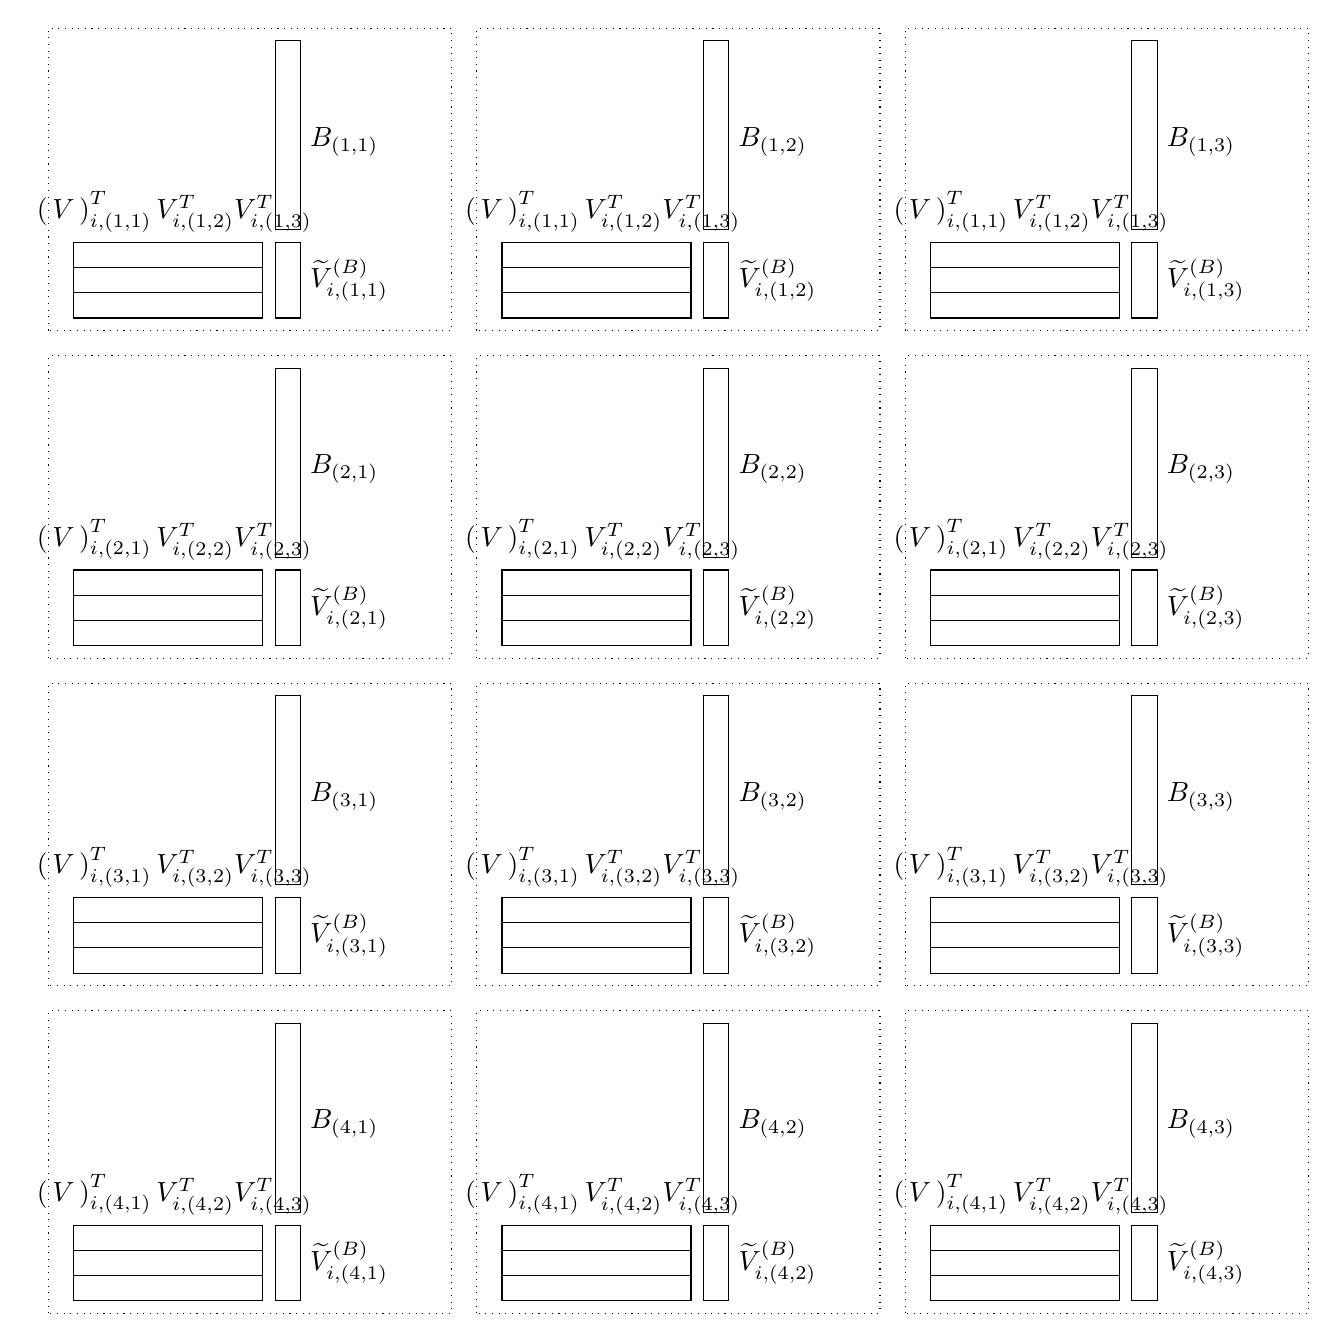
\begin{tikzpicture}[scale=16]
		% решетка процессов
		\draw [dotted] ( 0.00, 0.00 ) rectangle ( 0.32, 0.24 );
		\draw [dotted] ( 0.34, 0.00 ) rectangle ( 0.66, 0.24 );
		\draw [dotted] ( 0.68, 0.00 ) rectangle ( 1.00, 0.24 );
		\draw [dotted] ( 0.00, 0.26 ) rectangle ( 0.32, 0.50 );
		\draw [dotted] ( 0.34, 0.26 ) rectangle ( 0.66, 0.50 );
		\draw [dotted] ( 0.68, 0.26 ) rectangle ( 1.00, 0.50 );
		\draw [dotted] ( 0.00, 0.52 ) rectangle ( 0.32, 0.76 );
		\draw [dotted] ( 0.34, 0.52 ) rectangle ( 0.66, 0.76 );
		\draw [dotted] ( 0.68, 0.52 ) rectangle ( 1.00, 0.76 );
		\draw [dotted] ( 0.00, 0.78 ) rectangle ( 0.32, 1.02 );
		\draw [dotted] ( 0.34, 0.78 ) rectangle ( 0.66, 1.02 );
		\draw [dotted] ( 0.68, 0.78 ) rectangle ( 1.00, 1.02 );

		% процесс ( 1, 1 )
		\draw ( 0.02, 0.79 ) rectangle ( 0.17, 0.81 );
		\draw ( 0.02, 0.81 ) rectangle ( 0.17, 0.83 );
		\draw ( 0.02, 0.83 ) rectangle ( 0.17, 0.85 );
		\node [above] at ( 0.10, 0.85 ) {$\begin{pmatrix} V_{i,(1,1)}^T \\ V_{i,(1,2)}^T \\ V_{i,(1,3)}^T \end{pmatrix}$};
		\draw ( 0.18, 0.86 ) rectangle ( 0.20, 1.01 ) node [right] at ( 0.20, 0.93 ) {$B_{(1,1)}$};
		\draw ( 0.18, 0.79 ) rectangle ( 0.20, 0.85 ) node [right] at ( 0.20, 0.82 ) {$\widetilde{V}_{i,(1,1)}^{(B)}$};

		% процесс ( 1, 2 )
		\draw ( 0.36, 0.79 ) rectangle ( 0.51, 0.81 );
		\draw ( 0.36, 0.81 ) rectangle ( 0.51, 0.83 );
		\draw ( 0.36, 0.83 ) rectangle ( 0.51, 0.85 );
		\node [above] at ( 0.44, 0.85 ) {$\begin{pmatrix} V_{i,(1,1)}^T \\ V_{i,(1,2)}^T \\ V_{i,(1,3)}^T \end{pmatrix}$};
		\draw ( 0.52, 0.86 ) rectangle ( 0.54, 1.01 ) node [right] at ( 0.54, 0.93 ) {$B_{(1,2)}$};
		\draw ( 0.52, 0.79 ) rectangle ( 0.54, 0.85 ) node [right] at ( 0.54, 0.82 ) {$\widetilde{V}_{i,(1,2)}^{(B)}$};

		% процесс ( 1, 3 )
		\draw ( 0.70, 0.79 ) rectangle ( 0.85, 0.81 );
		\draw ( 0.70, 0.81 ) rectangle ( 0.85, 0.83 );
		\draw ( 0.70, 0.83 ) rectangle ( 0.85, 0.85 );
		\node [above] at ( 0.78, 0.85 ) {$\begin{pmatrix} V_{i,(1,1)}^T \\ V_{i,(1,2)}^T \\ V_{i,(1,3)}^T \end{pmatrix}$};
		\draw ( 0.86, 0.86 ) rectangle ( 0.88, 1.01 ) node [right] at ( 0.88, 0.93 ) {$B_{(1,3)}$};
		\draw ( 0.86, 0.79 ) rectangle ( 0.88, 0.85 ) node [right] at ( 0.88, 0.82 ) {$\widetilde{V}_{i,(1,3)}^{(B)}$};

		% процесс ( 2, 1 )
		\draw ( 0.02, 0.53 ) rectangle ( 0.17, 0.55 );
		\draw ( 0.02, 0.55 ) rectangle ( 0.17, 0.57 );
		\draw ( 0.02, 0.57 ) rectangle ( 0.17, 0.59 );
		\node [above] at ( 0.10, 0.59 ) {$\begin{pmatrix} V_{i,(2,1)}^T \\ V_{i,(2,2)}^T \\ V_{i,(2,3)}^T \end{pmatrix}$};
		\draw ( 0.18, 0.60 ) rectangle ( 0.20, 0.75 ) node [right] at ( 0.20, 0.67 ) {$B_{(2,1)}$};
		\draw ( 0.18, 0.53 ) rectangle ( 0.20, 0.59 ) node [right] at ( 0.20, 0.56 ) {$\widetilde{V}_{i,(2,1)}^{(B)}$};

		% процесс ( 2, 2 )
		\draw ( 0.36, 0.53 ) rectangle ( 0.51, 0.55 );
		\draw ( 0.36, 0.55 ) rectangle ( 0.51, 0.57 );
		\draw ( 0.36, 0.57 ) rectangle ( 0.51, 0.59 );
		\node [above] at ( 0.44, 0.59 ) {$\begin{pmatrix} V_{i,(2,1)}^T \\ V_{i,(2,2)}^T \\ V_{i,(2,3)}^T \end{pmatrix}$};
		\draw ( 0.52, 0.60 ) rectangle ( 0.54, 0.75 ) node [right] at ( 0.54, 0.67 ) {$B_{(2,2)}$};
		\draw ( 0.52, 0.53 ) rectangle ( 0.54, 0.59 ) node [right] at ( 0.54, 0.56 ) {$\widetilde{V}_{i,(2,2)}^{(B)}$};

		% процесс ( 2, 3 )
		\draw ( 0.70, 0.53 ) rectangle ( 0.85, 0.55 );
		\draw ( 0.70, 0.55 ) rectangle ( 0.85, 0.57 );
		\draw ( 0.70, 0.57 ) rectangle ( 0.85, 0.59 );
		\node [above] at ( 0.78, 0.59 ) {$\begin{pmatrix} V_{i,(2,1)}^T \\ V_{i,(2,2)}^T \\ V_{i,(2,3)}^T \end{pmatrix}$};
		\draw ( 0.86, 0.60 ) rectangle ( 0.88, 0.75 ) node [right] at ( 0.88, 0.67 ) {$B_{(2,3)}$};
		\draw ( 0.86, 0.53 ) rectangle ( 0.88, 0.59 ) node [right] at ( 0.88, 0.56 ) {$\widetilde{V}_{i,(2,3)}^{(B)}$};

		% процесс ( 3, 1 )
		\draw ( 0.02, 0.27 ) rectangle ( 0.17, 0.29 );
		\draw ( 0.02, 0.29 ) rectangle ( 0.17, 0.31 );
		\draw ( 0.02, 0.31 ) rectangle ( 0.17, 0.33 );
		\node [above] at ( 0.10, 0.33 ) {$\begin{pmatrix} V_{i,(3,1)}^T \\ V_{i,(3,2)}^T \\ V_{i,(3,3)}^T \end{pmatrix}$};
		\draw ( 0.18, 0.34 ) rectangle ( 0.20, 0.49 ) node [right] at ( 0.20, 0.41 ) {$B_{(3,1)}$};
		\draw ( 0.18, 0.27 ) rectangle ( 0.20, 0.33 ) node [right] at ( 0.20, 0.30 ) {$\widetilde{V}_{i,(3,1)}^{(B)}$};

		% процесс ( 3, 2 )
		\draw ( 0.36, 0.27 ) rectangle ( 0.51, 0.29 );
		\draw ( 0.36, 0.29 ) rectangle ( 0.51, 0.31 );
		\draw ( 0.36, 0.31 ) rectangle ( 0.51, 0.33 );
		\node [above] at ( 0.44, 0.33 ) {$\begin{pmatrix} V_{i,(3,1)}^T \\ V_{i,(3,2)}^T \\ V_{i,(3,3)}^T \end{pmatrix}$};
		\draw ( 0.52, 0.34 ) rectangle ( 0.54, 0.49 ) node [right] at ( 0.54, 0.41 ) {$B_{(3,2)}$};
		\draw ( 0.52, 0.27 ) rectangle ( 0.54, 0.33 ) node [right] at ( 0.54, 0.30 ) {$\widetilde{V}_{i,(3,2)}^{(B)}$};

		% процесс ( 3, 3 )
		\draw ( 0.70, 0.27 ) rectangle ( 0.85, 0.29 );
		\draw ( 0.70, 0.29 ) rectangle ( 0.85, 0.31 );
		\draw ( 0.70, 0.31 ) rectangle ( 0.85, 0.33 );
		\node [above] at ( 0.78, 0.33 ) {$\begin{pmatrix} V_{i,(3,1)}^T \\ V_{i,(3,2)}^T \\ V_{i,(3,3)}^T \end{pmatrix}$};
		\draw ( 0.86, 0.34 ) rectangle ( 0.88, 0.49 ) node [right] at ( 0.88, 0.41 ) {$B_{(3,3)}$};
		\draw ( 0.86, 0.27 ) rectangle ( 0.88, 0.33 ) node [right] at ( 0.88, 0.30 ) {$\widetilde{V}_{i,(3,3)}^{(B)}$};

		% процесс ( 4, 1 )
		\draw ( 0.02, 0.01 ) rectangle ( 0.17, 0.03 );
		\draw ( 0.02, 0.03 ) rectangle ( 0.17, 0.05 );
		\draw ( 0.02, 0.05 ) rectangle ( 0.17, 0.07 );
		\node [above] at ( 0.10, 0.07 ) {$\begin{pmatrix} V_{i,(4,1)}^T \\ V_{i,(4,2)}^T \\ V_{i,(4,3)}^T \end{pmatrix}$};
		\draw ( 0.18, 0.08 ) rectangle ( 0.20, 0.23 ) node [right] at ( 0.20, 0.15 ) {$B_{(4,1)}$};
		\draw ( 0.18, 0.01 ) rectangle ( 0.20, 0.07 ) node [right] at ( 0.20, 0.04 ) {$\widetilde{V}_{i,(4,1)}^{(B)}$};

		% процесс ( 4, 2 )
		\draw ( 0.36, 0.01 ) rectangle ( 0.51, 0.03 );
		\draw ( 0.36, 0.03 ) rectangle ( 0.51, 0.05 );
		\draw ( 0.36, 0.05 ) rectangle ( 0.51, 0.07 );
		\node [above] at ( 0.44, 0.07 ) {$\begin{pmatrix} V_{i,(4,1)}^T \\ V_{i,(4,2)}^T \\ V_{i,(4,3)}^T \end{pmatrix}$};
		\draw ( 0.52, 0.08 ) rectangle ( 0.54, 0.23 ) node [right] at ( 0.54, 0.15 ) {$B_{(4,2)}$};
		\draw ( 0.52, 0.01 ) rectangle ( 0.54, 0.07 ) node [right] at ( 0.54, 0.04 ) {$\widetilde{V}_{i,(4,2)}^{(B)}$};

		% процесс ( 4, 3 )
		\draw ( 0.70, 0.01 ) rectangle ( 0.85, 0.03 );
		\draw ( 0.70, 0.03 ) rectangle ( 0.85, 0.05 );
		\draw ( 0.70, 0.05 ) rectangle ( 0.85, 0.07 );
		\node [above] at ( 0.78, 0.07 ) {$\begin{pmatrix} V_{i,(4,1)}^T \\ V_{i,(4,2)}^T \\ V_{i,(4,3)}^T \end{pmatrix}$};
		\draw ( 0.86, 0.08 ) rectangle ( 0.88, 0.23 ) node [right] at ( 0.88, 0.15 ) {$B_{(4,3)}$};
		\draw ( 0.86, 0.01 ) rectangle ( 0.88, 0.07 ) node [right] at ( 0.88, 0.04 ) {$\widetilde{V}_{i,(4,3)}^{(B)}$};
	\end{tikzpicture}
	\caption{Вычисление $V_i^T B$: умножение}
\end{figure}

\begin{figure}
	\begin{tikzpicture}[scale=16]
		% решетка процессов
		\draw [dotted] ( 0.00, 0.00 ) rectangle ( 0.32, 0.24 );
		\draw [dotted] ( 0.34, 0.00 ) rectangle ( 0.66, 0.24 );
		\draw [dotted] ( 0.68, 0.00 ) rectangle ( 1.00, 0.24 );
		\draw [dotted] ( 0.00, 0.26 ) rectangle ( 0.32, 0.50 );
		\draw [dotted] ( 0.34, 0.26 ) rectangle ( 0.66, 0.50 );
		\draw [dotted] ( 0.68, 0.26 ) rectangle ( 1.00, 0.50 );
		\draw [dotted] ( 0.00, 0.52 ) rectangle ( 0.32, 0.76 );
		\draw [dotted] ( 0.34, 0.52 ) rectangle ( 0.66, 0.76 );
		\draw [dotted] ( 0.68, 0.52 ) rectangle ( 1.00, 0.76 );
		\draw [dotted] ( 0.00, 0.78 ) rectangle ( 0.32, 1.02 );
		\draw [dotted] ( 0.34, 0.78 ) rectangle ( 0.66, 1.02 );
		\draw [dotted] ( 0.68, 0.78 ) rectangle ( 1.00, 1.02 );

		% процесс ( 1, 1 )
		\draw ( 0.18, 0.79 ) rectangle ( 0.20, 0.85 ) node [above] at ( 0.19, 0.85 ) {$\begin{array}{l} \widetilde{V}_{i,(1,1)}^{(B)} \\ + \widetilde{V}_{i,(2,1)}^{(B)} \end{array}$};

		% процесс ( 1, 2 )
		\draw ( 0.52, 0.79 ) rectangle ( 0.54, 0.85 ) node [above] at ( 0.53, 0.85 ) {$\begin{array}{l} \widetilde{V}_{i,(1,2)}^{(B)} \\ + \widetilde{V}_{i,(2,2)}^{(B)} \end{array}$};

		% процесс ( 1, 3 )
		\draw ( 0.86, 0.79 ) rectangle ( 0.88, 0.85 ) node [above] at ( 0.87, 0.85 ) {$\begin{array}{l} \widetilde{V}_{i,(1,3)}^{(B)} \\ + \widetilde{V}_{i,(2,3)}^{(B)} \end{array}$};

		% процесс ( 2, 1 )
		\draw ( 0.18, 0.53 ) rectangle ( 0.20, 0.59 ) node [above] at ( 0.19, 0.59 ) {$\widetilde{V}_{i,(2,1)}^{(B)}$};
		\draw [->] ( 0.20, 0.56 ) to [ out = 0, in = 0 ] ( 0.20, 0.82 );

		% процесс ( 2, 2 )
		\draw ( 0.52, 0.53 ) rectangle ( 0.54, 0.59 ) node [above] at ( 0.53, 0.59 ) {$\widetilde{V}_{i,(2,2)}^{(B)}$};
		\draw [->] ( 0.54, 0.56 ) to [ out = 0, in = 0 ] ( 0.54, 0.82 );

		% процесс ( 2, 3 )
		\draw ( 0.86, 0.53 ) rectangle ( 0.88, 0.59 ) node [above] at ( 0.87, 0.59 ) {$\widetilde{V}_{i,(2,3)}^{(B)}$};
		\draw [->] ( 0.88, 0.56 ) to [ out = 0, in = 0 ] ( 0.88, 0.82 );

		% процесс ( 3, 1 )
		\draw ( 0.18, 0.27 ) rectangle ( 0.20, 0.33 ) node [above] at ( 0.19, 0.33 ) {$\begin{array}{l} \widetilde{V}_{i,(3,1)}^{(B)} \\ + \widetilde{V}_{i,(4,1)}^{(B)} \end{array}$};

		% процесс ( 3, 2 )
		\draw ( 0.52, 0.27 ) rectangle ( 0.54, 0.33 ) node [above] at ( 0.53, 0.33 ) {$\begin{array}{l} \widetilde{V}_{i,(3,2)}^{(B)} \\ + \widetilde{V}_{i,(4,2)}^{(B)} \end{array}$};

		% процесс ( 3, 3 )
		\draw ( 0.86, 0.27 ) rectangle ( 0.88, 0.33 ) node [above] at ( 0.87, 0.33 ) {$\begin{array}{l} \widetilde{V}_{i,(3,3)}^{(B)} \\ + \widetilde{V}_{i,(4,3)}^{(B)} \end{array}$};

		% процесс ( 4, 1 )
		\draw ( 0.18, 0.01 ) rectangle ( 0.20, 0.07 ) node [above] at ( 0.19, 0.07 ) {$\widetilde{V}_{i,(4,1)}^{(B)}$};
		\draw [->] ( 0.20, 0.04 ) to [ out = 0, in = 0 ] ( 0.20, 0.30 );

		% процесс ( 4, 2 )
		\draw ( 0.52, 0.01 ) rectangle ( 0.54, 0.07 ) node [above] at ( 0.53, 0.07 ) {$\widetilde{V}_{i,(4,2)}^{(B)}$};
		\draw [->] ( 0.54, 0.04 ) to [ out = 0, in = 0 ] ( 0.54, 0.30 );

		% процесс ( 4, 3 )
		\draw ( 0.86, 0.01 ) rectangle ( 0.88, 0.07 ) node [above] at ( 0.87, 0.07 ) {$\widetilde{V}_{i,(4,3)}^{(B)}$};
		\draw [->] ( 0.88, 0.04 ) to [ out = 0, in = 0 ] ( 0.88, 0.30 );
	\end{tikzpicture}
	\caption{Вычисление $V_i^T B$: суммирование, шаг 1}
\end{figure}

\begin{figure}
	\begin{tikzpicture}[scale=16]
		% решетка процессов
		\draw [dotted] ( 0.00, 0.00 ) rectangle ( 0.32, 0.24 );
		\draw [dotted] ( 0.34, 0.00 ) rectangle ( 0.66, 0.24 );
		\draw [dotted] ( 0.68, 0.00 ) rectangle ( 1.00, 0.24 );
		\draw [dotted] ( 0.00, 0.26 ) rectangle ( 0.32, 0.50 );
		\draw [dotted] ( 0.34, 0.26 ) rectangle ( 0.66, 0.50 );
		\draw [dotted] ( 0.68, 0.26 ) rectangle ( 1.00, 0.50 );
		\draw [dotted] ( 0.00, 0.52 ) rectangle ( 0.32, 0.76 );
		\draw [dotted] ( 0.34, 0.52 ) rectangle ( 0.66, 0.76 );
		\draw [dotted] ( 0.68, 0.52 ) rectangle ( 1.00, 0.76 );
		\draw [dotted] ( 0.00, 0.78 ) rectangle ( 0.32, 1.02 );
		\draw [dotted] ( 0.34, 0.78 ) rectangle ( 0.66, 1.02 );
		\draw [dotted] ( 0.68, 0.78 ) rectangle ( 1.00, 1.02 );

		% процесс ( 1, 1 )
		\draw ( 0.18, 0.79 ) rectangle ( 0.20, 0.85 ) node [above] at ( 0.19, 0.85 ) {$\begin{array}{l} \widetilde{V}_{i,(1,1)}^{(B)} \\ + \widetilde{V}_{i,(2,1)}^{(B)} \\ + \widetilde{V}_{i,(3,1)}^{(B)} \\ + \widetilde{V}_{i,(4,1)}^{(B)} \end{array}$};
		\node [left] at ( 0.18, 0.82 ) {$V_{i,(1,1)}^{(B)}$};

		% процесс ( 1, 2 )
		\draw ( 0.52, 0.79 ) rectangle ( 0.54, 0.85 ) node [above] at ( 0.53, 0.85 ) {$\begin{array}{l} \widetilde{V}_{i,(1,2)}^{(B)} \\ + \widetilde{V}_{i,(2,2)}^{(B)} \\ + \widetilde{V}_{i,(3,2)}^{(B)} \\ + \widetilde{V}_{i,(4,2)}^{(B)} \end{array}$};
		\node [left] at ( 0.52, 0.82 ) {$V_{i,(1,2)}^{(B)}$};

		% процесс ( 1, 3 )
		\draw ( 0.86, 0.79 ) rectangle ( 0.88, 0.85 ) node [above] at ( 0.87, 0.85 ) {$\begin{array}{l} \widetilde{V}_{i,(1,3)}^{(B)} \\ + \widetilde{V}_{i,(2,3)}^{(B)} \\ + \widetilde{V}_{i,(3,3)}^{(B)} \\ + \widetilde{V}_{i,(4,3)}^{(B)} \end{array}$};
		\node [left] at ( 0.86, 0.82 ) {$V_{i,(1,3)}^{(B)}$};

		% процесс ( 2, 1 )

		% процесс ( 2, 2 )

		% процесс ( 2, 3 )

		% процесс ( 3, 1 )
		\draw ( 0.18, 0.27 ) rectangle ( 0.20, 0.33 ) node [above] at ( 0.19, 0.33 ) {$\begin{array}{l} \widetilde{V}_{i,(3,1)}^{(B)} \\ + \widetilde{V}_{i,(4,1)}^{(B)} \end{array}$};
		\draw [->] ( 0.20, 0.30 ) to [ out = 0, in = 0 ] ( 0.20, 0.82 );

		% процесс ( 3, 2 )
		\draw ( 0.52, 0.27 ) rectangle ( 0.54, 0.33 ) node [above] at ( 0.53, 0.33 ) {$\begin{array}{l} \widetilde{V}_{i,(3,2)}^{(B)} \\ + \widetilde{V}_{i,(4,2)}^{(B)} \end{array}$};
		\draw [->] ( 0.54, 0.30 ) to [ out = 0, in = 0 ] ( 0.54, 0.82 );

		% процесс ( 3, 3 )
		\draw ( 0.86, 0.27 ) rectangle ( 0.88, 0.33 ) node [above] at ( 0.87, 0.33 ) {$\begin{array}{l} \widetilde{V}_{i,(3,3)}^{(B)} \\ + \widetilde{V}_{i,(4,3)}^{(B)} \end{array}$};
		\draw [->] ( 0.88, 0.30 ) to [ out = 0, in = 0 ] ( 0.88, 0.82 );

		% процесс ( 4, 1 )

		% процесс ( 4, 2 )

		% процесс ( 4, 3 )
	\end{tikzpicture}
	\caption{Вычисление $V_i^T B$: суммирование, шаг 2}
\end{figure}

\begin{figure}
	\begin{tikzpicture}[scale=16]
		% решетка процессов
		\draw [dotted] ( 0.00, 0.00 ) rectangle ( 0.32, 0.24 );
		\draw [dotted] ( 0.34, 0.00 ) rectangle ( 0.66, 0.24 );
		\draw [dotted] ( 0.68, 0.00 ) rectangle ( 1.00, 0.24 );
		\draw [dotted] ( 0.00, 0.26 ) rectangle ( 0.32, 0.50 );
		\draw [dotted] ( 0.34, 0.26 ) rectangle ( 0.66, 0.50 );
		\draw [dotted] ( 0.68, 0.26 ) rectangle ( 1.00, 0.50 );
		\draw [dotted] ( 0.00, 0.52 ) rectangle ( 0.32, 0.76 );
		\draw [dotted] ( 0.34, 0.52 ) rectangle ( 0.66, 0.76 );
		\draw [dotted] ( 0.68, 0.52 ) rectangle ( 1.00, 0.76 );
		\draw [dotted] ( 0.00, 0.78 ) rectangle ( 0.32, 1.02 );
		\draw [dotted] ( 0.34, 0.78 ) rectangle ( 0.66, 1.02 );
		\draw [dotted] ( 0.68, 0.78 ) rectangle ( 1.00, 1.02 );

		% процесс ( 1, 1 )
		\draw ( 0.18, 0.79 ) rectangle ( 0.20, 0.85 ) node [left] at ( 0.18, 0.82 ) {$V_{i,(1,1)}^{(B)}$};
		\draw [->] ( 0.20, 0.82 ) to [ out = 0, in = 0 ] ( 0.20, 0.30 );

		% процесс ( 1, 2 )
		\draw ( 0.52, 0.79 ) rectangle ( 0.54, 0.85 ) node [left] at ( 0.52, 0.82 ) {$V_{i,(1,2)}^{(B)}$};
		\draw [->] ( 0.54, 0.82 ) to [ out = 0, in = 0 ] ( 0.54, 0.30 );

		% процесс ( 1, 3 )
		\draw ( 0.86, 0.79 ) rectangle ( 0.88, 0.85 ) node [left] at ( 0.86, 0.82 ) {$V_{i,(1,3)}^{(B)}$};
		\draw [->] ( 0.88, 0.82 ) to [ out = 0, in = 0 ] ( 0.88, 0.30 );

		% процесс ( 2, 1 )

		% процесс ( 2, 2 )

		% процесс ( 2, 3 )

		% процесс ( 3, 1 )
		\draw ( 0.18, 0.27 ) rectangle ( 0.20, 0.33 ) node [left] at ( 0.18, 0.30 ) {$V_{i,(1,1)}^{(B)}$};

		% процесс ( 3, 2 )
		\draw ( 0.52, 0.27 ) rectangle ( 0.54, 0.33 ) node [left] at ( 0.52, 0.30 ) {$V_{i,(1,2)}^{(B)}$};

		% процесс ( 3, 3 )
		\draw ( 0.86, 0.27 ) rectangle ( 0.88, 0.33 ) node [left] at ( 0.86, 0.30 ) {$V_{i,(1,3)}^{(B)}$};

		% процесс ( 4, 1 )

		% процесс ( 4, 2 )

		% процесс ( 4, 3 )
	\end{tikzpicture}
	\caption{Вычисление $V_i^T B$: распределение, шаг 1}
\end{figure}

\begin{figure}
	\begin{tikzpicture}[scale=16]
		% решетка процессов
		\draw [dotted] ( 0.00, 0.00 ) rectangle ( 0.32, 0.24 );
		\draw [dotted] ( 0.34, 0.00 ) rectangle ( 0.66, 0.24 );
		\draw [dotted] ( 0.68, 0.00 ) rectangle ( 1.00, 0.24 );
		\draw [dotted] ( 0.00, 0.26 ) rectangle ( 0.32, 0.50 );
		\draw [dotted] ( 0.34, 0.26 ) rectangle ( 0.66, 0.50 );
		\draw [dotted] ( 0.68, 0.26 ) rectangle ( 1.00, 0.50 );
		\draw [dotted] ( 0.00, 0.52 ) rectangle ( 0.32, 0.76 );
		\draw [dotted] ( 0.34, 0.52 ) rectangle ( 0.66, 0.76 );
		\draw [dotted] ( 0.68, 0.52 ) rectangle ( 1.00, 0.76 );
		\draw [dotted] ( 0.00, 0.78 ) rectangle ( 0.32, 1.02 );
		\draw [dotted] ( 0.34, 0.78 ) rectangle ( 0.66, 1.02 );
		\draw [dotted] ( 0.68, 0.78 ) rectangle ( 1.00, 1.02 );

		% процесс ( 1, 1 )
		\draw ( 0.18, 0.79 ) rectangle ( 0.20, 0.85 ) node [left] at ( 0.18, 0.82 ) {$V_{i,(1,1)}^{(B)}$};
		\draw [->] ( 0.20, 0.82 ) to [ out = 0, in = 0 ] ( 0.20, 0.56 );

		% процесс ( 1, 2 )
		\draw ( 0.52, 0.79 ) rectangle ( 0.54, 0.85 ) node [left] at ( 0.52, 0.82 ) {$V_{i,(1,2)}^{(B)}$};
		\draw [->] ( 0.54, 0.82 ) to [ out = 0, in = 0 ] ( 0.54, 0.56 );

		% процесс ( 1, 3 )
		\draw ( 0.86, 0.79 ) rectangle ( 0.88, 0.85 ) node [left] at ( 0.86, 0.82 ) {$V_{i,(1,3)}^{(B)}$};
		\draw [->] ( 0.88, 0.82 ) to [ out = 0, in = 0 ] ( 0.88, 0.56 );

		% процесс ( 2, 1 )
		\draw ( 0.18, 0.53 ) rectangle ( 0.20, 0.59 ) node [left] at ( 0.18, 0.56 ) {$V_{i,(1,1)}^{(B)}$};

		% процесс ( 2, 2 )
		\draw ( 0.52, 0.53 ) rectangle ( 0.54, 0.59 ) node [left] at ( 0.52, 0.56 ) {$V_{i,(1,2)}^{(B)}$};

		% процесс ( 2, 3 )
		\draw ( 0.86, 0.53 ) rectangle ( 0.88, 0.59 ) node [left] at ( 0.86, 0.56 ) {$V_{i,(1,3)}^{(B)}$};

		% процесс ( 3, 1 )
		\draw ( 0.18, 0.27 ) rectangle ( 0.20, 0.33 ) node [left] at ( 0.18, 0.30 ) {$V_{i,(1,1)}^{(B)}$};
		\draw [->] ( 0.20, 0.30 ) to [ out = 0, in = 0 ] ( 0.20, 0.04 );

		% процесс ( 3, 2 )
		\draw ( 0.52, 0.27 ) rectangle ( 0.54, 0.33 ) node [left] at ( 0.52, 0.30 ) {$V_{i,(1,2)}^{(B)}$};
		\draw [->] ( 0.54, 0.30 ) to [ out = 0, in = 0 ] ( 0.54, 0.04 );

		% процесс ( 3, 3 )
		\draw ( 0.86, 0.27 ) rectangle ( 0.88, 0.33 ) node [left] at ( 0.86, 0.30 ) {$V_{i,(1,3)}^{(B)}$};
		\draw [->] ( 0.88, 0.30 ) to [ out = 0, in = 0 ] ( 0.88, 0.04 );

		% процесс ( 4, 1 )
		\draw ( 0.18, 0.01 ) rectangle ( 0.20, 0.07 ) node [left] at ( 0.18, 0.04 ) {$V_{i,(1,1)}^{(B)}$};

		% процесс ( 4, 2 )
		\draw ( 0.52, 0.01 ) rectangle ( 0.54, 0.07 ) node [left] at ( 0.52, 0.04 ) {$V_{i,(1,2)}^{(B)}$};

		% процесс ( 4, 3 )
		\draw ( 0.86, 0.01 ) rectangle ( 0.88, 0.07 ) node [left] at ( 0.86, 0.04 ) {$V_{i,(1,3)}^{(B)}$};
	\end{tikzpicture}
	\caption{Вычисление $V_i^T B$: распределение, шаг 2}
\end{figure}

\subsection{Вычисление $V_i^{(Q)} = V_i Q_i^{(inv)}$ (вариант 1)}
$$
	\begin{pmatrix}
		V_{i,(1,1)}^{(Q)} & V_{i,(1,2)}^{(Q)} & V_{i,(1,3)}^{(Q)} \\
		V_{i,(2,1)}^{(Q)} & V_{i,(2,2)}^{(Q)} & V_{i,(2,3)}^{(Q)} \\
		V_{i,(3,1)}^{(Q)} & V_{i,(3,2)}^{(Q)} & V_{i,(3,3)}^{(Q)} \\
		V_{i,(4,1)}^{(Q)} & V_{i,(4,2)}^{(Q)} & V_{i,(4,3)}^{(Q)}
	\end{pmatrix}
	=
	\begin{pmatrix}
		V_{i,(1,1)} & V_{i,(1,2)} & V_{i,(1,3)} \\
		V_{i,(2,1)} & V_{i,(2,2)} & V_{i,(2,3)} \\
		V_{i,(3,1)} & V_{i,(3,2)} & V_{i,(3,3)} \\
		V_{i,(4,1)} & V_{i,(4,2)} & V_{i,(4,3)}
	\end{pmatrix}
	\times
	\begin{pmatrix}
		Q_{i,(1,1)}^{(inv)} & Q_{i,(1,2)}^{(inv)} & Q_{i,(1,3)}^{(inv)}
	\end{pmatrix}
$$

\begin{figure}
	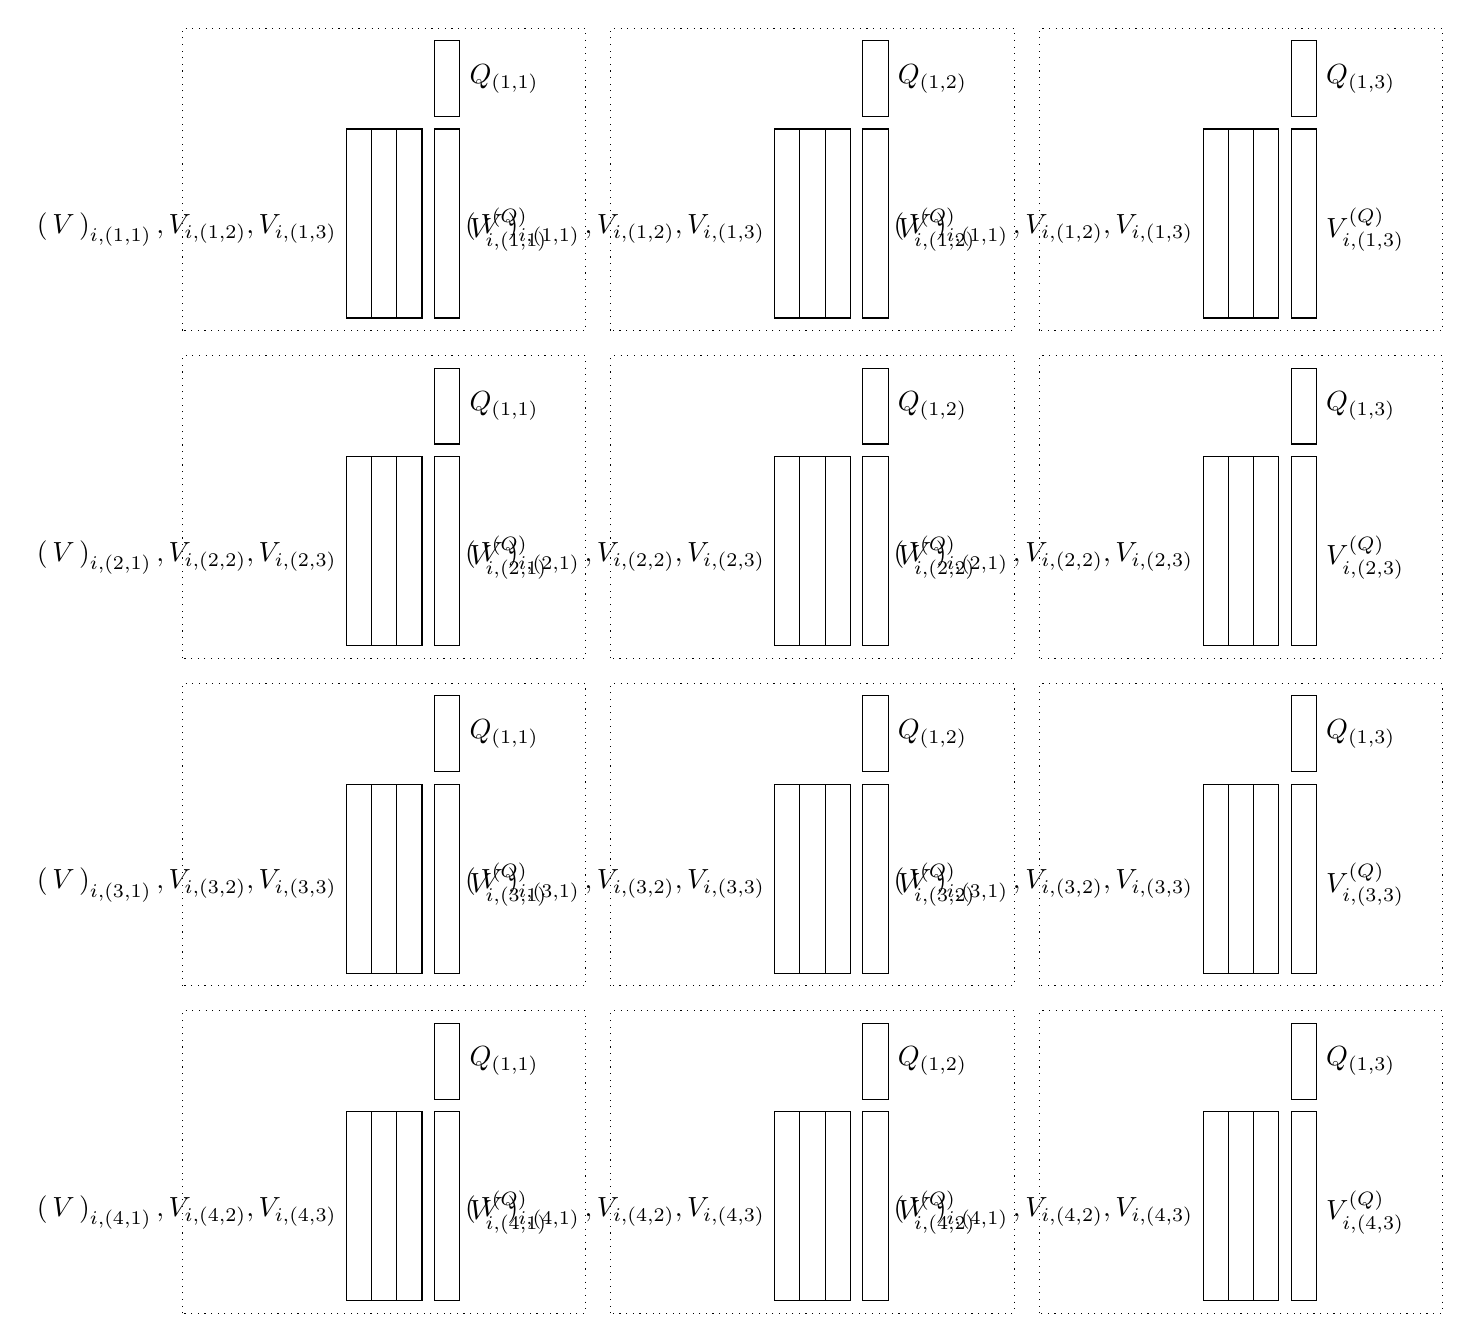
\begin{tikzpicture}[scale=16]
		% решетка процессов
		\draw [dotted] ( 0.00, 0.00 ) rectangle ( 0.32, 0.24 );
		\draw [dotted] ( 0.34, 0.00 ) rectangle ( 0.66, 0.24 );
		\draw [dotted] ( 0.68, 0.00 ) rectangle ( 1.00, 0.24 );
		\draw [dotted] ( 0.00, 0.26 ) rectangle ( 0.32, 0.50 );
		\draw [dotted] ( 0.34, 0.26 ) rectangle ( 0.66, 0.50 );
		\draw [dotted] ( 0.68, 0.26 ) rectangle ( 1.00, 0.50 );
		\draw [dotted] ( 0.00, 0.52 ) rectangle ( 0.32, 0.76 );
		\draw [dotted] ( 0.34, 0.52 ) rectangle ( 0.66, 0.76 );
		\draw [dotted] ( 0.68, 0.52 ) rectangle ( 1.00, 0.76 );
		\draw [dotted] ( 0.00, 0.78 ) rectangle ( 0.32, 1.02 );
		\draw [dotted] ( 0.34, 0.78 ) rectangle ( 0.66, 1.02 );
		\draw [dotted] ( 0.68, 0.78 ) rectangle ( 1.00, 1.02 );

		% процесс ( 1, 1 )
		\draw ( 0.13, 0.79 ) rectangle ( 0.15, 0.94 );
		\draw ( 0.15, 0.79 ) rectangle ( 0.17, 0.94 );
		\draw ( 0.17, 0.79 ) rectangle ( 0.19, 0.94 );
		\node [left] at ( 0.13, 0.86 ) {$\begin{pmatrix} V_{i,(1,1)}, \\ V_{i,(1,2)}, \\ V_{i,(1,3)} \end{pmatrix}$};
		\draw ( 0.20, 0.95 ) rectangle ( 0.22, 1.01 ) node [right] at ( 0.22, 0.98 ) {$Q_{(1,1)}$};
		\draw ( 0.20, 0.79 ) rectangle ( 0.22, 0.94 ) node [right] at ( 0.22, 0.86 ) {$V_{i,(1,1)}^{(Q)}$};

		% процесс ( 1, 2 )
		\draw ( 0.47, 0.79 ) rectangle ( 0.49, 0.94 );
		\draw ( 0.49, 0.79 ) rectangle ( 0.51, 0.94 );
		\draw ( 0.51, 0.79 ) rectangle ( 0.53, 0.94 );
		\node [left] at ( 0.47, 0.86 ) {$\begin{pmatrix} V_{i,(1,1)}, \\ V_{i,(1,2)}, \\ V_{i,(1,3)} \end{pmatrix}$};
		\draw ( 0.54, 0.95 ) rectangle ( 0.56, 1.01 ) node [right] at ( 0.56, 0.98 ) {$Q_{(1,2)}$};
		\draw ( 0.54, 0.79 ) rectangle ( 0.56, 0.94 ) node [right] at ( 0.56, 0.86 ) {$V_{i,(1,2)}^{(Q)}$};

		% процесс ( 1, 3 )
		\draw ( 0.81, 0.79 ) rectangle ( 0.83, 0.94 );
		\draw ( 0.83, 0.79 ) rectangle ( 0.85, 0.94 );
		\draw ( 0.85, 0.79 ) rectangle ( 0.87, 0.94 );
		\node [left] at ( 0.81, 0.86 ) {$\begin{pmatrix} V_{i,(1,1)}, \\ V_{i,(1,2)}, \\ V_{i,(1,3)} \end{pmatrix}$};
		\draw ( 0.88, 0.95 ) rectangle ( 0.90, 1.01 ) node [right] at ( 0.90, 0.98 ) {$Q_{(1,3)}$};
		\draw ( 0.88, 0.79 ) rectangle ( 0.90, 0.94 ) node [right] at ( 0.90, 0.86 ) {$V_{i,(1,3)}^{(Q)}$};

		% процесс ( 2, 1 )
		\draw ( 0.13, 0.53 ) rectangle ( 0.15, 0.68 );
		\draw ( 0.15, 0.53 ) rectangle ( 0.17, 0.68 );
		\draw ( 0.17, 0.53 ) rectangle ( 0.19, 0.68 );
		\node [left] at ( 0.13, 0.60 ) {$\begin{pmatrix} V_{i,(2,1)}, \\ V_{i,(2,2)}, \\ V_{i,(2,3)} \end{pmatrix}$};
		\draw ( 0.20, 0.69 ) rectangle ( 0.22, 0.75 ) node [right] at ( 0.22, 0.72 ) {$Q_{(1,1)}$};
		\draw ( 0.20, 0.53 ) rectangle ( 0.22, 0.68 ) node [right] at ( 0.22, 0.60 ) {$V_{i,(2,1)}^{(Q)}$};

		% процесс ( 2, 2 )
		\draw ( 0.47, 0.53 ) rectangle ( 0.49, 0.68 );
		\draw ( 0.49, 0.53 ) rectangle ( 0.51, 0.68 );
		\draw ( 0.51, 0.53 ) rectangle ( 0.53, 0.68 );
		\node [left] at ( 0.47, 0.60 ) {$\begin{pmatrix} V_{i,(2,1)}, \\ V_{i,(2,2)}, \\ V_{i,(2,3)} \end{pmatrix}$};
		\draw ( 0.54, 0.69 ) rectangle ( 0.56, 0.75 ) node [right] at ( 0.56, 0.72 ) {$Q_{(1,2)}$};
		\draw ( 0.54, 0.53 ) rectangle ( 0.56, 0.68 ) node [right] at ( 0.56, 0.60 ) {$V_{i,(2,2)}^{(Q)}$};

		% процесс ( 2, 3 )
		\draw ( 0.81, 0.53 ) rectangle ( 0.83, 0.68 );
		\draw ( 0.83, 0.53 ) rectangle ( 0.85, 0.68 );
		\draw ( 0.85, 0.53 ) rectangle ( 0.87, 0.68 );
		\node [left] at ( 0.81, 0.60 ) {$\begin{pmatrix} V_{i,(2,1)}, \\ V_{i,(2,2)}, \\ V_{i,(2,3)} \end{pmatrix}$};
		\draw ( 0.88, 0.69 ) rectangle ( 0.90, 0.75 ) node [right] at ( 0.90, 0.72 ) {$Q_{(1,3)}$};
		\draw ( 0.88, 0.53 ) rectangle ( 0.90, 0.68 ) node [right] at ( 0.90, 0.60 ) {$V_{i,(2,3)}^{(Q)}$};

		% процесс ( 3, 1 )
		\draw ( 0.13, 0.27 ) rectangle ( 0.15, 0.42 );
		\draw ( 0.15, 0.27 ) rectangle ( 0.17, 0.42 );
		\draw ( 0.17, 0.27 ) rectangle ( 0.19, 0.42 );
		\node [left] at ( 0.13, 0.34 ) {$\begin{pmatrix} V_{i,(3,1)}, \\ V_{i,(3,2)}, \\ V_{i,(3,3)} \end{pmatrix}$};
		\draw ( 0.20, 0.43 ) rectangle ( 0.22, 0.49 ) node [right] at ( 0.22, 0.46 ) {$Q_{(1,1)}$};
		\draw ( 0.20, 0.27 ) rectangle ( 0.22, 0.42 ) node [right] at ( 0.22, 0.34 ) {$V_{i,(3,1)}^{(Q)}$};

		% процесс ( 3, 2 )
		\draw ( 0.47, 0.27 ) rectangle ( 0.49, 0.42 );
		\draw ( 0.49, 0.27 ) rectangle ( 0.51, 0.42 );
		\draw ( 0.51, 0.27 ) rectangle ( 0.53, 0.42 );
		\node [left] at ( 0.47, 0.34 ) {$\begin{pmatrix} V_{i,(3,1)}, \\ V_{i,(3,2)}, \\ V_{i,(3,3)} \end{pmatrix}$};
		\draw ( 0.54, 0.43 ) rectangle ( 0.56, 0.49 ) node [right] at ( 0.56, 0.46 ) {$Q_{(1,2)}$};
		\draw ( 0.54, 0.27 ) rectangle ( 0.56, 0.42 ) node [right] at ( 0.56, 0.34 ) {$V_{i,(3,2)}^{(Q)}$};

		% процесс ( 3, 3 )
		\draw ( 0.81, 0.27 ) rectangle ( 0.83, 0.42 );
		\draw ( 0.83, 0.27 ) rectangle ( 0.85, 0.42 );
		\draw ( 0.85, 0.27 ) rectangle ( 0.87, 0.42 );
		\node [left] at ( 0.81, 0.34 ) {$\begin{pmatrix} V_{i,(3,1)}, \\ V_{i,(3,2)}, \\ V_{i,(3,3)} \end{pmatrix}$};
		\draw ( 0.88, 0.43 ) rectangle ( 0.90, 0.49 ) node [right] at ( 0.90, 0.46 ) {$Q_{(1,3)}$};
		\draw ( 0.88, 0.27 ) rectangle ( 0.90, 0.42 ) node [right] at ( 0.90, 0.34 ) {$V_{i,(3,3)}^{(Q)}$};

		% процесс ( 4, 1 )
		\draw ( 0.13, 0.01 ) rectangle ( 0.15, 0.16 );
		\draw ( 0.15, 0.01 ) rectangle ( 0.17, 0.16 );
		\draw ( 0.17, 0.01 ) rectangle ( 0.19, 0.16 );
		\node [left] at ( 0.13, 0.08 ) {$\begin{pmatrix} V_{i,(4,1)}, \\ V_{i,(4,2)}, \\ V_{i,(4,3)} \end{pmatrix}$};
		\draw ( 0.20, 0.17 ) rectangle ( 0.22, 0.23 ) node [right] at ( 0.22, 0.20 ) {$Q_{(1,1)}$};
		\draw ( 0.20, 0.01 ) rectangle ( 0.22, 0.16 ) node [right] at ( 0.22, 0.08 ) {$V_{i,(4,1)}^{(Q)}$};

		% процесс ( 4, 2 )
		\draw ( 0.47, 0.01 ) rectangle ( 0.49, 0.16 );
		\draw ( 0.49, 0.01 ) rectangle ( 0.51, 0.16 );
		\draw ( 0.51, 0.01 ) rectangle ( 0.53, 0.16 );
		\node [left] at ( 0.47, 0.08 ) {$\begin{pmatrix} V_{i,(4,1)}, \\ V_{i,(4,2)}, \\ V_{i,(4,3)} \end{pmatrix}$};
		\draw ( 0.54, 0.17 ) rectangle ( 0.56, 0.23 ) node [right] at ( 0.56, 0.20 ) {$Q_{(1,2)}$};
		\draw ( 0.54, 0.01 ) rectangle ( 0.56, 0.16 ) node [right] at ( 0.56, 0.08 ) {$V_{i,(4,2)}^{(Q)}$};

		% процесс ( 4, 3 )
		\draw ( 0.81, 0.01 ) rectangle ( 0.83, 0.16 );
		\draw ( 0.83, 0.01 ) rectangle ( 0.85, 0.16 );
		\draw ( 0.85, 0.01 ) rectangle ( 0.87, 0.16 );
		\node [left] at ( 0.81, 0.08 ) {$\begin{pmatrix} V_{i,(4,1)}, \\ V_{i,(4,2)}, \\ V_{i,(4,3)} \end{pmatrix}$};
		\draw ( 0.88, 0.17 ) rectangle ( 0.90, 0.23 ) node [right] at ( 0.90, 0.20 ) {$Q_{(1,3)}$};
		\draw ( 0.88, 0.01 ) rectangle ( 0.90, 0.16 ) node [right] at ( 0.90, 0.08 ) {$V_{i,(4,3)}^{(Q)}$};

	\end{tikzpicture}
	\caption{Вычисление $V_i^{(Q)}$ (вариант 1): умножение}
\end{figure}

\begin{figure}
	\begin{tikzpicture}[scale=16]
		% решетка процессов
		\draw [dotted] ( 0.00, 0.00 ) rectangle ( 0.32, 0.24 );
		\draw [dotted] ( 0.34, 0.00 ) rectangle ( 0.66, 0.24 );
		\draw [dotted] ( 0.68, 0.00 ) rectangle ( 1.00, 0.24 );
		\draw [dotted] ( 0.00, 0.26 ) rectangle ( 0.32, 0.50 );
		\draw [dotted] ( 0.34, 0.26 ) rectangle ( 0.66, 0.50 );
		\draw [dotted] ( 0.68, 0.26 ) rectangle ( 1.00, 0.50 );
		\draw [dotted] ( 0.00, 0.52 ) rectangle ( 0.32, 0.76 );
		\draw [dotted] ( 0.34, 0.52 ) rectangle ( 0.66, 0.76 );
		\draw [dotted] ( 0.68, 0.52 ) rectangle ( 1.00, 0.76 );
		\draw [dotted] ( 0.00, 0.78 ) rectangle ( 0.32, 1.02 );
		\draw [dotted] ( 0.34, 0.78 ) rectangle ( 0.66, 1.02 );
		\draw [dotted] ( 0.68, 0.78 ) rectangle ( 1.00, 1.02 );

		% процесс ( 1, 1 )
		\draw [dotted] ( 0.24, 0.79 ) rectangle ( 0.30, 0.94 );
		\draw ( 0.24, 0.79 ) rectangle ( 0.26, 0.94 );
		\draw ( 0.28, 0.79 ) rectangle ( 0.30, 0.94 );
		\draw [->] ( 0.26, 0.89 ) -- ( 0.58, 0.89 );
		\node [above left] at ( 0.30, 0.94 ) {$\begin{pmatrix} V_{i,(1,1)}^{(Q)} & - & V_{i,(1,3)}^{(Q)} \end{pmatrix}$};

		% процесс ( 1, 2 )
		\draw [dotted] ( 0.58, 0.79 ) rectangle ( 0.64, 0.94 );
		\draw ( 0.58, 0.79 ) rectangle ( 0.60, 0.94 );
		\draw ( 0.60, 0.79 ) rectangle ( 0.62, 0.94 );
		\draw [->] ( 0.62, 0.84 ) -- ( 0.94, 0.84 );
		\node [above left] at ( 0.64, 0.94 ) {$\begin{pmatrix} V_{i,(1,1)}^{(Q)} & V_{i,(1,2)}^{(Q)} & - \end{pmatrix}$};

		% процесс ( 1, 3 )
		\draw [dotted] ( 0.92, 0.79 ) rectangle ( 0.98, 0.94 );
		\draw ( 0.94, 0.79 ) rectangle ( 0.96, 0.94 );
		\draw ( 0.96, 0.79 ) rectangle ( 0.98, 0.94 );
		\draw [->] ( 0.97, 0.79 ) -- ( 0.97, 0.77 ) -- ( 0.29, 0.77 ) -- ( 0.29, 0.79 );
		\node [above left] at ( 0.98, 0.94 ) {$\begin{pmatrix} - & V_{i,(1,2)}^{(Q)} & V_{i,(1,3)}^{(Q)} \end{pmatrix}$};

		% процесс ( 2, 1 )
		\draw [dotted] ( 0.24, 0.53 ) rectangle ( 0.30, 0.68 );
		\draw ( 0.24, 0.53 ) rectangle ( 0.26, 0.68 );
		\draw ( 0.28, 0.53 ) rectangle ( 0.30, 0.68 );
		\draw [->] ( 0.26, 0.63 ) -- ( 0.58, 0.63 );
		\node [above left] at ( 0.30, 0.68 ) {$\begin{pmatrix} V_{i,(2,1)}^{(Q)} & - & V_{i,(2,3)}^{(Q)} \end{pmatrix}$};

		% процесс ( 2, 2 )
		\draw [dotted] ( 0.58, 0.53 ) rectangle ( 0.64, 0.68 );
		\draw ( 0.58, 0.53 ) rectangle ( 0.60, 0.68 );
		\draw ( 0.60, 0.53 ) rectangle ( 0.62, 0.68 );
		\draw [->] ( 0.62, 0.58 ) -- ( 0.94, 0.58 );
		\node [above left] at ( 0.64, 0.68 ) {$\begin{pmatrix} V_{i,(2,1)}^{(Q)} & V_{i,(2,2)}^{(Q)} & - \end{pmatrix}$};

		% процесс ( 2, 3 )
		\draw [dotted] ( 0.92, 0.53 ) rectangle ( 0.98, 0.68 );
		\draw ( 0.94, 0.53 ) rectangle ( 0.96, 0.68 );
		\draw ( 0.96, 0.53 ) rectangle ( 0.98, 0.68 );
		\draw [->] ( 0.97, 0.53 ) -- ( 0.97, 0.51 ) -- ( 0.29, 0.51 ) -- ( 0.29, 0.53 );
		\node [above left] at ( 0.98, 0.68 ) {$\begin{pmatrix} - & V_{i,(2,2)}^{(Q)} & V_{i,(2,3)}^{(Q)} \end{pmatrix}$};

		% процесс ( 3, 1 )
		\draw [dotted] ( 0.24, 0.27 ) rectangle ( 0.30, 0.42 );
		\draw ( 0.24, 0.27 ) rectangle ( 0.26, 0.42 );
		\draw ( 0.28, 0.27 ) rectangle ( 0.30, 0.42 );
		\draw [->] ( 0.26, 0.36 ) -- ( 0.58, 0.36 );
		\node [above left] at ( 0.30, 0.42 ) {$\begin{pmatrix} V_{i,(3,1)}^{(Q)} & - & V_{i,(3,3)}^{(Q)} \end{pmatrix}$};

		% процесс ( 3, 2 )
		\draw [dotted] ( 0.58, 0.27 ) rectangle ( 0.64, 0.42 );
		\draw ( 0.58, 0.27 ) rectangle ( 0.60, 0.42 );
		\draw ( 0.60, 0.27 ) rectangle ( 0.62, 0.42 );
		\draw [->] ( 0.62, 0.31 ) -- ( 0.94, 0.31 );
		\node [above left] at ( 0.65, 0.42 ) {$\begin{pmatrix} V_{i,(3,1)}^{(Q)} & V_{i,(3,2)}^{(Q)} & - \end{pmatrix}$};

		% процесс ( 3, 3 )
		\draw [dotted] ( 0.92, 0.27 ) rectangle ( 0.98, 0.42 );
		\draw ( 0.94, 0.27 ) rectangle ( 0.96, 0.42 );
		\draw ( 0.96, 0.27 ) rectangle ( 0.98, 0.42 );
		\draw [->] ( 0.97, 0.27 ) -- ( 0.97, 0.25 ) -- ( 0.29, 0.25 ) -- ( 0.29, 0.27 );
		\node [above left] at ( 0.98, 0.42 ) {$\begin{pmatrix} - & V_{i,(3,2)}^{(Q)} & V_{i,(3,3)}^{(Q)} \end{pmatrix}$};

		% процесс ( 4, 1 )
		\draw [dotted] ( 0.24, 0.01 ) rectangle ( 0.30, 0.16 );
		\draw ( 0.24, 0.01 ) rectangle ( 0.26, 0.16 );
		\draw ( 0.28, 0.01 ) rectangle ( 0.30, 0.16 );
		\draw [->] ( 0.26, 0.10 ) -- ( 0.58, 0.10 );
		\node [above left] at ( 0.30, 0.16 ) {$\begin{pmatrix} V_{i,(4,1)}^{(Q)} & - & V_{i,(4,3)}^{(Q)} \end{pmatrix}$};

		% процесс ( 4, 2 )
		\draw [dotted] ( 0.58, 0.01 ) rectangle ( 0.64, 0.16 );
		\draw ( 0.58, 0.01 ) rectangle ( 0.60, 0.16 );
		\draw ( 0.60, 0.01 ) rectangle ( 0.62, 0.16 );
		\draw [->] ( 0.62, 0.05 ) -- ( 0.94, 0.05 );
		\node [above left] at ( 0.64, 0.16 ) {$\begin{pmatrix} V_{i,(4,1)}^{(Q)} & V_{i,(4,2)}^{(Q)} & - \end{pmatrix}$};

		% процесс ( 4, 3 )
		\draw [dotted] ( 0.92, 0.01 ) rectangle ( 0.98, 0.16 );
		\draw ( 0.94, 0.01 ) rectangle ( 0.96, 0.16 );
		\draw ( 0.96, 0.01 ) rectangle ( 0.98, 0.16 );
		\draw [->] ( 0.97, 0.01 ) -- ( 0.97, -0.01 ) -- ( 0.29, -0.01 ) -- ( 0.29, 0.01 );
		\node [above left] at ( 0.98, 0.16 ) {$\begin{pmatrix} - & V_{i,(4,2)}^{(Q)} & V_{i,(4,3)}^{(Q)} \end{pmatrix}$};

	\end{tikzpicture}
	\caption{Вычисление $V_i^{(Q)}$ (вариант 1): сбор, шаг 1}
\end{figure}

\begin{figure}
	\begin{tikzpicture}[scale=16]
		% решетка процессов
		\draw [dotted] ( 0.00, 0.00 ) rectangle ( 0.32, 0.24 );
		\draw [dotted] ( 0.34, 0.00 ) rectangle ( 0.66, 0.24 );
		\draw [dotted] ( 0.68, 0.00 ) rectangle ( 1.00, 0.24 );
		\draw [dotted] ( 0.00, 0.26 ) rectangle ( 0.32, 0.50 );
		\draw [dotted] ( 0.34, 0.26 ) rectangle ( 0.66, 0.50 );
		\draw [dotted] ( 0.68, 0.26 ) rectangle ( 1.00, 0.50 );
		\draw [dotted] ( 0.00, 0.52 ) rectangle ( 0.32, 0.76 );
		\draw [dotted] ( 0.34, 0.52 ) rectangle ( 0.66, 0.76 );
		\draw [dotted] ( 0.68, 0.52 ) rectangle ( 1.00, 0.76 );
		\draw [dotted] ( 0.00, 0.78 ) rectangle ( 0.32, 1.02 );
		\draw [dotted] ( 0.34, 0.78 ) rectangle ( 0.66, 1.02 );
		\draw [dotted] ( 0.68, 0.78 ) rectangle ( 1.00, 1.02 );

		% процесс ( 1, 1 )
		\draw ( 0.24, 0.79 ) rectangle ( 0.26, 0.94 );
		\draw ( 0.26, 0.79 ) rectangle ( 0.28, 0.94 );
		\draw ( 0.28, 0.79 ) rectangle ( 0.30, 0.94 );
		\draw [->] ( 0.30, 0.89 ) -- ( 0.62, 0.89 );
		\node [above left] at ( 0.30, 0.94 ) {$\begin{pmatrix} V_{i,(1,1)}^{(Q)} & V_{i,(1,2)}^{(Q)} & V_{i,(1,3)}^{(Q)} \end{pmatrix}$};

		% процесс ( 1, 2 )
		\draw ( 0.58, 0.79 ) rectangle ( 0.60, 0.94 );
		\draw ( 0.60, 0.79 ) rectangle ( 0.62, 0.94 );
		\draw ( 0.62, 0.79 ) rectangle ( 0.64, 0.94 );
		\draw [->] ( 0.60, 0.84 ) -- ( 0.92, 0.84 );
		\node [above left] at ( 0.64, 0.94 ) {$\begin{pmatrix} V_{i,(1,1)}^{(Q)} & V_{i,(1,2)}^{(Q)} & V_{i,(1,3)}^{(Q)} \end{pmatrix}$};

		% процесс ( 1, 3 )
		\draw ( 0.92, 0.79 ) rectangle ( 0.94, 0.94 );
		\draw ( 0.94, 0.79 ) rectangle ( 0.96, 0.94 );
		\draw ( 0.96, 0.79 ) rectangle ( 0.98, 0.94 );
		\draw [->] ( 0.95, 0.79 ) -- ( 0.95, 0.77 ) -- ( 0.27, 0.77 ) -- ( 0.27, 0.79 );
		\node [above left] at ( 0.98, 0.94 ) {$\begin{pmatrix} V_{i,(1,1)}^{(Q)} & V_{i,(1,2)}^{(Q)} & V_{i,(1,3)}^{(Q)} \end{pmatrix}$};

		% процесс ( 2, 1 )
		\draw ( 0.24, 0.53 ) rectangle ( 0.26, 0.68 );
		\draw ( 0.26, 0.53 ) rectangle ( 0.28, 0.68 );
		\draw ( 0.28, 0.53 ) rectangle ( 0.30, 0.68 );
		\draw [->] ( 0.30, 0.63 ) -- ( 0.62, 0.63 );
		\node [above left] at ( 0.30, 0.68 ) {$\begin{pmatrix} V_{i,(2,1)}^{(Q)} & V_{i,(2,2)}^{(Q)} & V_{i,(2,3)}^{(Q)} \end{pmatrix}$};

		% процесс ( 2, 2 )
		\draw ( 0.58, 0.53 ) rectangle ( 0.60, 0.68 );
		\draw ( 0.60, 0.53 ) rectangle ( 0.62, 0.68 );
		\draw ( 0.62, 0.53 ) rectangle ( 0.64, 0.68 );
		\draw [->] ( 0.60, 0.58 ) -- ( 0.92, 0.58 );
		\node [above left] at ( 0.64, 0.68 ) {$\begin{pmatrix} V_{i,(2,1)}^{(Q)} & V_{i,(2,2)}^{(Q)} & V_{i,(2,3)}^{(Q)} \end{pmatrix}$};

		% процесс ( 2, 3 )
		\draw ( 0.92, 0.53 ) rectangle ( 0.94, 0.68 );
		\draw ( 0.94, 0.53 ) rectangle ( 0.96, 0.68 );
		\draw ( 0.96, 0.53 ) rectangle ( 0.98, 0.68 );
		\draw [->] ( 0.95, 0.53 ) -- ( 0.95, 0.51 ) -- ( 0.27, 0.51 ) -- ( 0.27, 0.53 );
		\node [above left] at ( 0.98, 0.68 ) {$\begin{pmatrix} V_{i,(2,1)}^{(Q)} & V_{i,(2,2)}^{(Q)} & V_{i,(2,3)}^{(Q)} \end{pmatrix}$};

		% процесс ( 3, 1 )
		\draw ( 0.24, 0.27 ) rectangle ( 0.26, 0.42 );
		\draw ( 0.26, 0.27 ) rectangle ( 0.28, 0.42 );
		\draw ( 0.28, 0.27 ) rectangle ( 0.30, 0.42 );
		\draw [->] ( 0.30, 0.36 ) -- ( 0.62, 0.36 );
		\node [above left] at ( 0.30, 0.42 ) {$\begin{pmatrix} V_{i,(3,1)}^{(Q)} & V_{i,(3,2)}^{(Q)} & V_{i,(3,3)}^{(Q)} \end{pmatrix}$};

		% процесс ( 3, 2 )
		\draw ( 0.58, 0.27 ) rectangle ( 0.60, 0.42 );
		\draw ( 0.60, 0.27 ) rectangle ( 0.62, 0.42 );
		\draw ( 0.62, 0.27 ) rectangle ( 0.64, 0.42 );
		\draw [->] ( 0.60, 0.31 ) -- ( 0.92, 0.31 );
		\node [above left] at ( 0.65, 0.42 ) {$\begin{pmatrix} V_{i,(3,1)}^{(Q)} & V_{i,(3,2)}^{(Q)} & V_{i,(3,3)}^{(Q)} \end{pmatrix}$};

		% процесс ( 3, 3 )
		\draw ( 0.92, 0.27 ) rectangle ( 0.94, 0.42 );
		\draw ( 0.94, 0.27 ) rectangle ( 0.96, 0.42 );
		\draw ( 0.96, 0.27 ) rectangle ( 0.98, 0.42 );
		\draw [->] ( 0.95, 0.27 ) -- ( 0.95, 0.25 ) -- ( 0.27, 0.25 ) -- ( 0.27, 0.27 );
		\node [above left] at ( 0.98, 0.42 ) {$\begin{pmatrix} V_{i,(3,1)}^{(Q)} & V_{i,(3,2)}^{(Q)} & V_{i,(3,3)}^{(Q)} \end{pmatrix}$};

		% процесс ( 4, 1 )
		\draw ( 0.24, 0.01 ) rectangle ( 0.26, 0.16 );
		\draw ( 0.26, 0.01 ) rectangle ( 0.28, 0.16 );
		\draw ( 0.28, 0.01 ) rectangle ( 0.30, 0.16 );
		\draw [->] ( 0.30,  0.10 ) -- ( 0.62, 0.10 );
		\node [above left] at ( 0.30, 0.16 ) {$\begin{pmatrix} V_{i,(4,1)}^{(Q)} & V_{i,(4,2)}^{(Q)} & V_{i,(4,3)}^{(Q)} \end{pmatrix}$};

		% процесс ( 4, 2 )
		\draw ( 0.58, 0.01 ) rectangle ( 0.60, 0.16 );
		\draw ( 0.60, 0.01 ) rectangle ( 0.62, 0.16 );
		\draw ( 0.62, 0.01 ) rectangle ( 0.64, 0.16 );
		\draw [->] ( 0.60, 0.05 ) -- ( 0.92, 0.05 );
		\node [above left] at ( 0.64, 0.16 ) {$\begin{pmatrix} V_{i,(4,1)}^{(Q)} & V_{i,(4,2)}^{(Q)} & V_{i,(4,3)}^{(Q)} \end{pmatrix}$};

		% процесс ( 4, 3 )
		\draw ( 0.92, 0.01 ) rectangle ( 0.94, 0.16 );
		\draw ( 0.94, 0.01 ) rectangle ( 0.96, 0.16 );
		\draw ( 0.96, 0.01 ) rectangle ( 0.98, 0.16 );
		\draw [->] ( 0.95, 0.01 ) -- ( 0.95, -0.01 ) -- ( 0.27, -0.01 ) -- ( 0.27, 0.01 );
		\node [above left] at ( 0.98, 0.16 ) {$\begin{pmatrix} V_{i,(4,1)}^{(Q)} & V_{i,(4,2)}^{(Q)} & V_{i,(4,3)}^{(Q)} \end{pmatrix}$};

	\end{tikzpicture}
	\caption{Вычисление $V_i^{(Q)}$ (вариант 1): сбор, шаг 2}
\end{figure}

\subsection{Вычисление $V_i^{(Q)} = V_i Q_i^{(inv)}$ (вариант 2)}

$$
	\begin{pmatrix}
		V_{i,(1,1)}^{(Q)} & V_{i,(1,2)}^{(Q)} & V_{i,(1,3)}^{(Q)} \\
		V_{i,(2,1)}^{(Q)} & V_{i,(2,2)}^{(Q)} & V_{i,(2,3)}^{(Q)} \\
		V_{i,(3,1)}^{(Q)} & V_{i,(3,2)}^{(Q)} & V_{i,(3,3)}^{(Q)} \\
		V_{i,(4,1)}^{(Q)} & V_{i,(4,2)}^{(Q)} & V_{i,(4,3)}^{(Q)}
	\end{pmatrix}
	=
	\begin{pmatrix}
		V_{i,(1,1)} & V_{i,(1,2)} & V_{i,(1,3)} \\
		V_{i,(2,1)} & V_{i,(2,2)} & V_{i,(2,3)} \\
		V_{i,(3,1)} & V_{i,(3,2)} & V_{i,(3,3)} \\
		V_{i,(4,1)} & V_{i,(4,2)} & V_{i,(4,3)}
	\end{pmatrix}
	\times
	\begin{pmatrix}
		Q_{i,(1,1)}^{(inv)} & Q_{i,(1,2)}^{(inv)} & Q_{i,(1,3)}^{(inv)} \\
		Q_{i,(2,1)}^{(inv)} & Q_{i,(2,2)}^{(inv)} & Q_{i,(2,3)}^{(inv)} \\
		Q_{i,(3,1)}^{(inv)} & Q_{i,(3,2)}^{(inv)} & Q_{i,(3,3)}^{(inv)}
	\end{pmatrix}
$$

$$
	\begin{pmatrix}
		\widetilde{V}_{i,(1,1)}^{(Q)} & \widetilde{V}_{i,(1,2)}^{(Q)} & \widetilde{V}_{i,(1,3)}^{(Q)} \\
		\widetilde{V}_{i,(2,1)}^{(Q)} & \widetilde{V}_{i,(2,2)}^{(Q)} & \widetilde{V}_{i,(2,3)}^{(Q)} \\
		\widetilde{V}_{i,(3,1)}^{(Q)} & \widetilde{V}_{i,(3,2)}^{(Q)} & \widetilde{V}_{i,(3,3)}^{(Q)} \\
		\widetilde{V}_{i,(4,1)}^{(Q)} & \widetilde{V}_{i,(4,2)}^{(Q)} & \widetilde{V}_{i,(4,3)}^{(Q)}
	\end{pmatrix}
	=
	\begin{pmatrix}
		V_{i,(1,1)} Q_{i,(1,1)}^{-1} & V_{i,(1,2)} Q_{i,(2,1)}^{-1} & V_{i,(1,3)} Q_{i,(3,1)}^{-1} \\
		V_{i,(2,1)} Q_{i,(1,1)}^{-1} & V_{i,(2,2)} Q_{i,(2,1)}^{-1} & V_{i,(2,3)} Q_{i,(3,1)}^{-1} \\
		V_{i,(3,1)} Q_{i,(1,1)}^{-1} & V_{i,(3,2)} Q_{i,(2,1)}^{-1} & V_{i,(3,3)} Q_{i,(3,1)}^{-1} \\
		V_{i,(4,1)} Q_{i,(1,1)}^{-1} & V_{i,(4,2)} Q_{i,(2,1)}^{-1} & V_{i,(4,3)} Q_{i,(3,1)}^{-1}
	\end{pmatrix}
$$

$$
	\begin{pmatrix}
		V_{i,(1,1)}^{(Q)} \\
		V_{i,(2,1)}^{(Q)} \\
		V_{i,(3,1)}^{(Q)} \\
		V_{i,(4,1)}^{(Q)}
	\end{pmatrix}
	=
	\begin{pmatrix}
		\widetilde{V}_{i,(1,1)}^Q + {}\widetilde{V}_{i,(1,2)}^Q + {}\widetilde{V}_{i,(1,3)}^Q \\
		\widetilde{V}_{i,(2,1)}^Q + {}\widetilde{V}_{i,(2,2)}^Q + {}\widetilde{V}_{i,(2,3)}^Q \\
		\widetilde{V}_{i,(3,1)}^Q + {}\widetilde{V}_{i,(3,2)}^Q + {}\widetilde{V}_{i,(3,3)}^Q \\
		\widetilde{V}_{i,(4,1)}^Q + {}\widetilde{V}_{i,(4,2)}^Q + {}\widetilde{V}_{i,(4,3)}^Q
	\end{pmatrix}
	=
	\begin{pmatrix}
		V_{i,(1,1)} Q_{i,(1,1)}^{-1} + V_{i,(1,2)} Q_{i,(2,1)}^{-1} + V_{i,(1,3)} Q_{i,(3,1)}^{-1} \\
		V_{i,(2,1)} Q_{i,(1,1)}^{-1} + V_{i,(2,2)} Q_{i,(2,1)}^{-1} + V_{i,(2,3)} Q_{i,(3,1)}^{-1} \\
		V_{i,(3,1)} Q_{i,(1,1)}^{-1} + V_{i,(3,2)} Q_{i,(2,1)}^{-1} + V_{i,(3,3)} Q_{i,(3,1)}^{-1} \\
		V_{i,(4,1)} Q_{i,(1,1)}^{-1} + V_{i,(4,2)} Q_{i,(2,1)}^{-1} + V_{i,(4,3)} Q_{i,(3,1)}^{-1}
	\end{pmatrix}
$$

\begin{figure}
	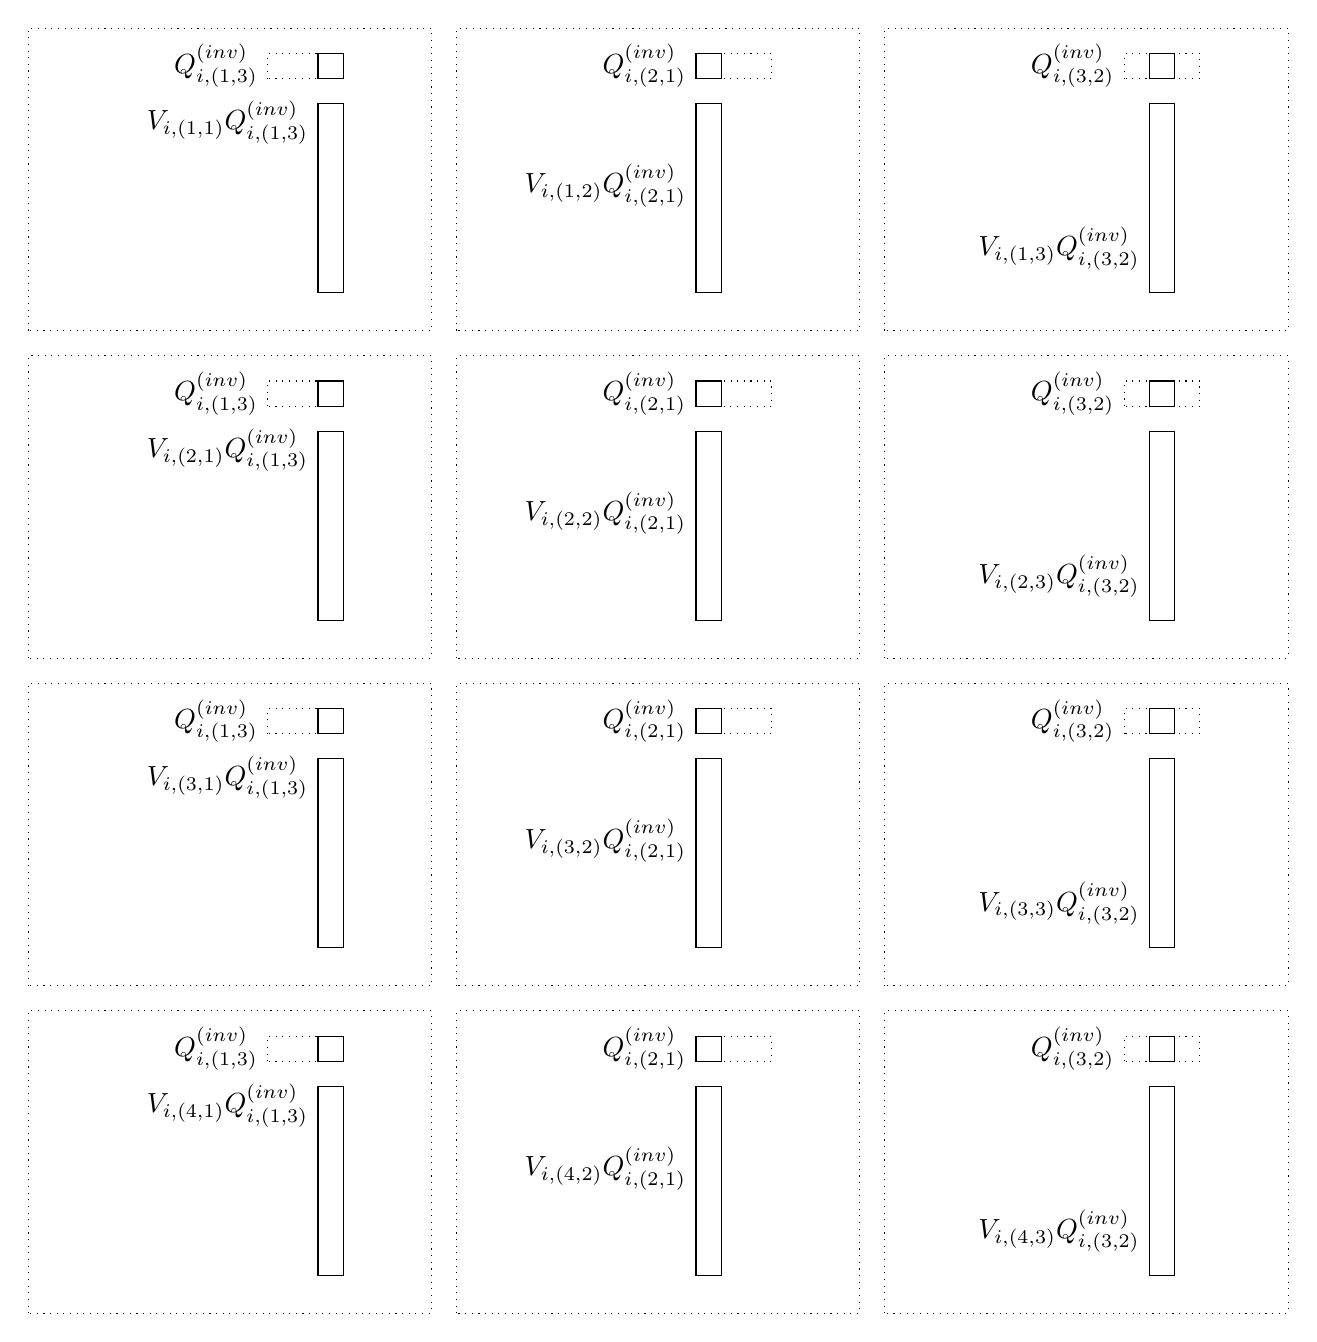
\begin{tikzpicture}[scale=16]
		% решетка процессов
		\draw [dotted] ( 0.00, 0.00 ) rectangle ( 0.32, 0.24 );
		\draw [dotted] ( 0.34, 0.00 ) rectangle ( 0.66, 0.24 );
		\draw [dotted] ( 0.68, 0.00 ) rectangle ( 1.00, 0.24 );
		\draw [dotted] ( 0.00, 0.26 ) rectangle ( 0.32, 0.50 );
		\draw [dotted] ( 0.34, 0.26 ) rectangle ( 0.66, 0.50 );
		\draw [dotted] ( 0.68, 0.26 ) rectangle ( 1.00, 0.50 );
		\draw [dotted] ( 0.00, 0.52 ) rectangle ( 0.32, 0.76 );
		\draw [dotted] ( 0.34, 0.52 ) rectangle ( 0.66, 0.76 );
		\draw [dotted] ( 0.68, 0.52 ) rectangle ( 1.00, 0.76 );
		\draw [dotted] ( 0.00, 0.78 ) rectangle ( 0.32, 1.02 );
		\draw [dotted] ( 0.34, 0.78 ) rectangle ( 0.66, 1.02 );
		\draw [dotted] ( 0.68, 0.78 ) rectangle ( 1.00, 1.02 );

		% процесс ( 1, 1 )
		\draw [dotted] ( 0.19, 0.98 ) rectangle ( 0.25, 1.00 );
		\draw ( 0.23, 0.98 ) rectangle ( 0.25, 1.00 ) node [left] at ( 0.19, 0.99 ) {$Q_{i,(1,3)}^{(inv)}$};
		\draw ( 0.23, 0.81 ) rectangle ( 0.25, 0.96 );
		\node [below left] at ( 0.23, 0.97 ) {$V_{i,(1,1)} Q_{i,(1,3)}^{(inv)}$};

		% процесс ( 1, 2 )
		\draw [dotted] ( 0.53, 0.98 ) rectangle ( 0.59, 1.00 );
		\draw ( 0.53, 0.98 ) rectangle ( 0.55, 1.00 ) node [left] at ( 0.53, 0.99 ) {$Q_{i,(2,1)}^{(inv)}$};
		\draw ( 0.53, 0.81 ) rectangle ( 0.55, 0.96 );
		\node [below left] at ( 0.53, 0.92 ) {$V_{i,(1,2)} Q_{i,(2,1)}^{(inv)}$};

		% процесс ( 1, 3 )
		\draw [dotted] ( 0.87, 0.98 ) rectangle ( 0.93, 1.00 );
		\draw ( 0.89, 0.98 ) rectangle ( 0.91, 1.00 ) node [left] at ( 0.87, 0.99 ) {$Q_{i,(3,2)}^{(inv)}$};
		\draw ( 0.89, 0.81 ) rectangle ( 0.91, 0.96 );
		\node [below left] at ( 0.89, 0.87 ) {$V_{i,(1,3)} Q_{i,(3,2)}^{(inv)}$};

		% процесс ( 2, 1 )
		\draw [dotted] ( 0.19, 0.72 ) rectangle ( 0.25, 0.74 );
		\draw ( 0.23, 0.72 ) rectangle ( 0.25, 0.74 ) node [left] at ( 0.19, 0.73 ) {$Q_{i,(1,3)}^{(inv)}$};
		\draw ( 0.23, 0.55 ) rectangle ( 0.25, 0.70 );
		\node [below left] at ( 0.23, 0.71 ) {$V_{i,(2,1)} Q_{i,(1,3)}^{(inv)}$};

		% процесс ( 2, 2 )
		\draw [dotted] ( 0.53, 0.72 ) rectangle ( 0.59, 0.74 );
		\draw ( 0.53, 0.72 ) rectangle ( 0.55, 0.74 ) node [left] at ( 0.53, 0.73 ) {$Q_{i,(2,1)}^{(inv)}$};
		\draw ( 0.53, 0.55 ) rectangle ( 0.55, 0.70 );
		\node [below left] at ( 0.53, 0.66 ) {$V_{i,(2,2)} Q_{i,(2,1)}^{(inv)}$};

		% процесс ( 2, 3 )
		\draw [dotted] ( 0.87, 0.72 ) rectangle ( 0.93, 0.74 );
		\draw ( 0.89, 0.72 ) rectangle ( 0.91, 0.74 ) node [left] at ( 0.87, 0.73 ) {$Q_{i,(3,2)}^{(inv)}$};
		\draw ( 0.89, 0.55 ) rectangle ( 0.91, 0.70 );
		\node [below left] at ( 0.89, 0.61 ) {$V_{i,(2,3)} Q_{i,(3,2)}^{(inv)}$};

		% процесс ( 3, 1 )
		\draw [dotted] ( 0.19, 0.46 ) rectangle ( 0.25, 0.48 );
		\draw ( 0.23, 0.46 ) rectangle ( 0.25, 0.48 ) node [left] at ( 0.19, 0.47 ) {$Q_{i,(1,3)}^{(inv)}$};
		\draw ( 0.23, 0.29 ) rectangle ( 0.25, 0.44 );
		\node [below left] at ( 0.23, 0.45 ) {$V_{i,(3,1)} Q_{i,(1,3)}^{(inv)}$};

		% процесс ( 3, 2 )
		\draw [dotted] ( 0.53, 0.46 ) rectangle ( 0.59, 0.48 );
		\draw ( 0.53, 0.46 ) rectangle ( 0.55, 0.48 ) node [left] at ( 0.53, 0.47 ) {$Q_{i,(2,1)}^{(inv)}$};
		\draw ( 0.53, 0.29 ) rectangle ( 0.55, 0.44 );
		\node [below left] at ( 0.53, 0.40 ) {$V_{i,(3,2)} Q_{i,(2,1)}^{(inv)}$};

		% процесс ( 3, 3 )
		\draw [dotted] ( 0.87, 0.46 ) rectangle ( 0.93, 0.48 );
		\draw ( 0.89, 0.46 ) rectangle ( 0.91, 0.48 ) node [left] at ( 0.87, 0.47 ) {$Q_{i,(3,2)}^{(inv)}$};
		\draw ( 0.89, 0.29 ) rectangle ( 0.91, 0.44 );
		\node [below left] at ( 0.89, 0.35 ) {$V_{i,(3,3)} Q_{i,(3,2)}^{(inv)}$};

		% процесс ( 4, 1 )
		\draw [dotted] ( 0.19, 0.20 ) rectangle ( 0.25, 0.22 );
		\draw ( 0.23, 0.20 ) rectangle ( 0.25, 0.22 ) node [left] at ( 0.19, 0.21 ) {$Q_{i,(1,3)}^{(inv)}$};
		\draw ( 0.23, 0.03 ) rectangle ( 0.25, 0.18 );
		\node [below left] at ( 0.23, 0.19 ) {$V_{i,(4,1)} Q_{i,(1,3)}^{(inv)}$};

		% процесс ( 4, 2 )
		\draw [dotted] ( 0.53, 0.20 ) rectangle ( 0.59, 0.22 );
		\draw ( 0.53, 0.20 ) rectangle ( 0.55, 0.22 ) node [left] at ( 0.53, 0.21 ) {$Q_{i,(2,1)}^{(inv)}$};
		\draw ( 0.53, 0.03 ) rectangle ( 0.55, 0.18 );
		\node [below left] at ( 0.53, 0.14 ) {$V_{i,(4,2)} Q_{i,(2,1)}^{(inv)}$};

		% процесс ( 4, 3 )
		\draw [dotted] ( 0.87, 0.20 ) rectangle ( 0.93, 0.22 );
		\draw ( 0.89, 0.20 ) rectangle ( 0.91, 0.22 ) node [left] at ( 0.87, 0.21 ) {$Q_{i,(3,2)}^{(inv)}$};
		\draw ( 0.89, 0.03 ) rectangle ( 0.91, 0.18 );
		\node [below left] at ( 0.89, 0.09 ) {$V_{i,(4,3)} Q_{i,(3,2)}^{(inv)}$};
	\end{tikzpicture}
	\caption{Вычисление $V_i^{(Q)}$ (вариант 2): шаг 1}
\end{figure}

\begin{figure}
	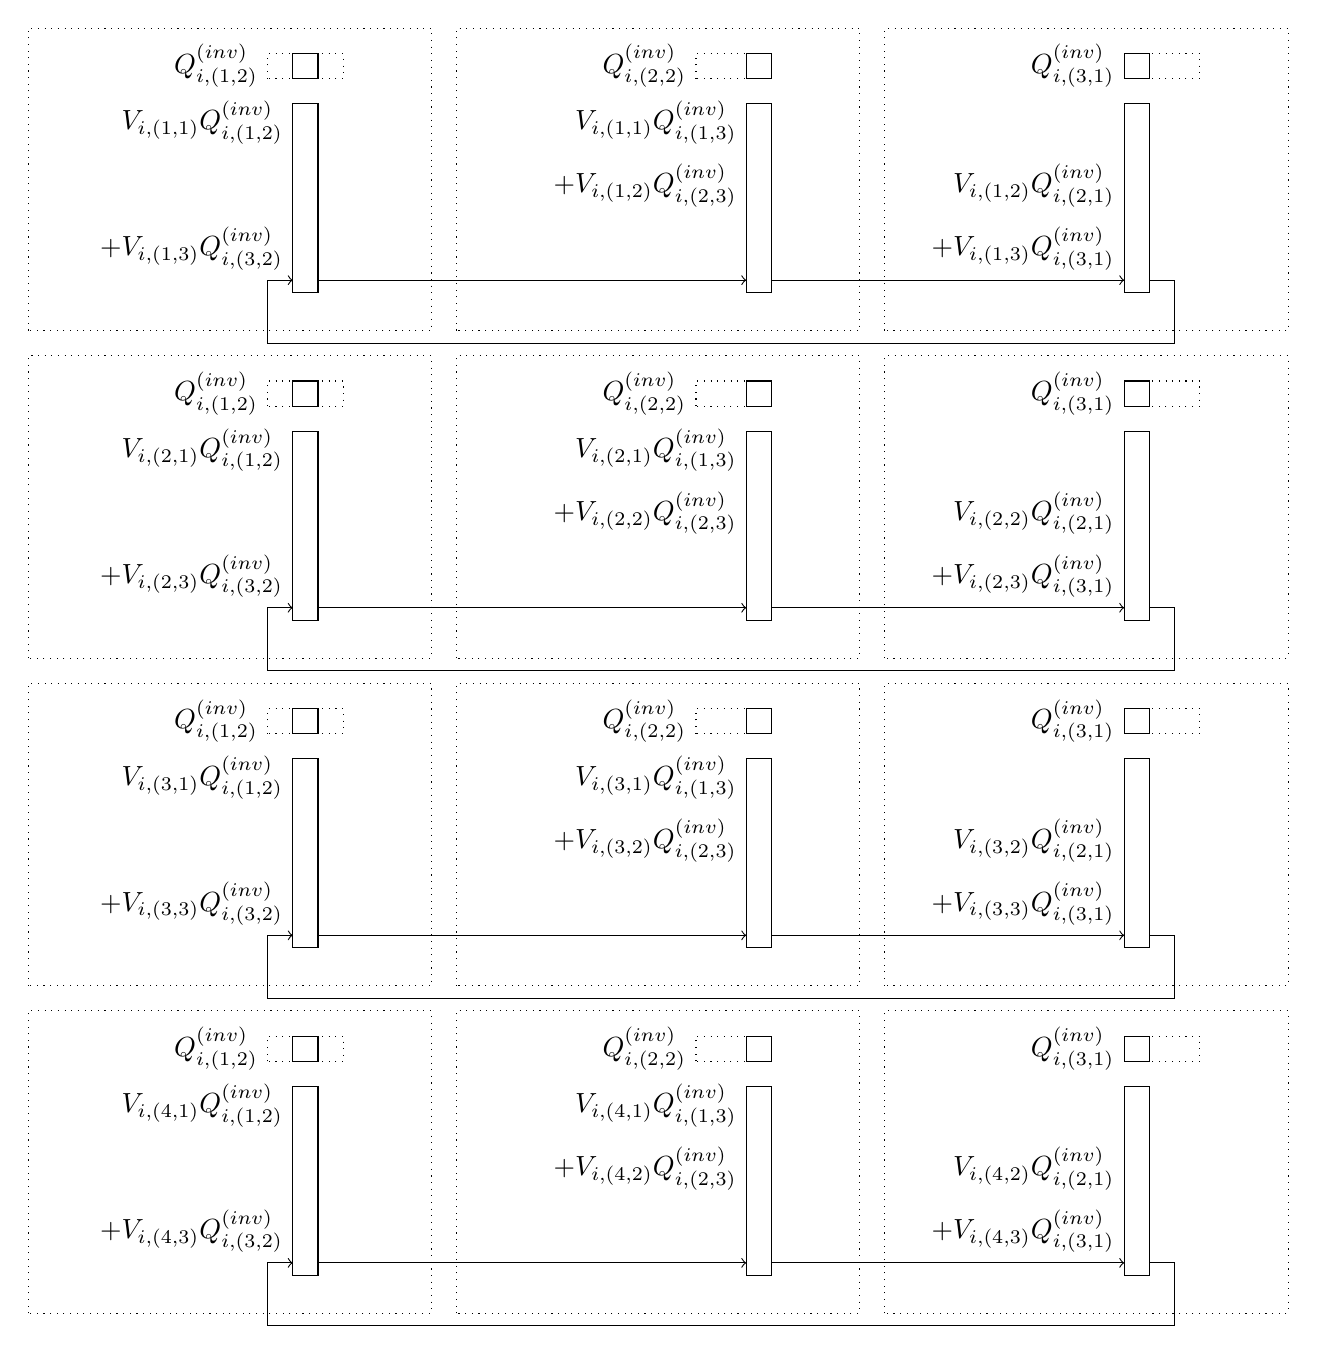
\begin{tikzpicture}[scale=16]
		% решетка процессов
		\draw [dotted] ( 0.00, 0.00 ) rectangle ( 0.32, 0.24 );
		\draw [dotted] ( 0.34, 0.00 ) rectangle ( 0.66, 0.24 );
		\draw [dotted] ( 0.68, 0.00 ) rectangle ( 1.00, 0.24 );
		\draw [dotted] ( 0.00, 0.26 ) rectangle ( 0.32, 0.50 );
		\draw [dotted] ( 0.34, 0.26 ) rectangle ( 0.66, 0.50 );
		\draw [dotted] ( 0.68, 0.26 ) rectangle ( 1.00, 0.50 );
		\draw [dotted] ( 0.00, 0.52 ) rectangle ( 0.32, 0.76 );
		\draw [dotted] ( 0.34, 0.52 ) rectangle ( 0.66, 0.76 );
		\draw [dotted] ( 0.68, 0.52 ) rectangle ( 1.00, 0.76 );
		\draw [dotted] ( 0.00, 0.78 ) rectangle ( 0.32, 1.02 );
		\draw [dotted] ( 0.34, 0.78 ) rectangle ( 0.66, 1.02 );
		\draw [dotted] ( 0.68, 0.78 ) rectangle ( 1.00, 1.02 );

		% процесс ( 1, 1 )
		\draw [dotted] ( 0.19, 0.98 ) rectangle ( 0.25, 1.00 );
		\draw ( 0.21, 0.98 ) rectangle ( 0.23, 1.00 ) node [left] at ( 0.19, 0.99 ) {$Q_{i,(1,2)}^{(inv)}$};
		\draw ( 0.21, 0.81 ) rectangle ( 0.23, 0.96 );
		\node [below left] at ( 0.21, 0.97 ) {$V_{i,(1,1)} Q_{i,(1,2)}^{(inv)}$};
		\node [below left] at ( 0.21, 0.87 ) {$+V_{i,(1,3)} Q_{i,(3,2)}^{(inv)}$};
		\draw [->] ( 0.23, 0.82 ) -- ( 0.57, 0.82 );

		% процесс ( 1, 2 )
		\draw [dotted] ( 0.53, 0.98 ) rectangle ( 0.59, 1.00 );
		\draw ( 0.57, 0.98 ) rectangle ( 0.59, 1.00 ) node [left] at ( 0.53, 0.99 ) {$Q_{i,(2,2)}^{(inv)}$};
		\draw ( 0.57, 0.81 ) rectangle ( 0.59, 0.96 );
		\node [below left] at ( 0.57, 0.97 ) {$V_{i,(1,1)} Q_{i,(1,3)}^{(inv)}$};
		\node [below left] at ( 0.57, 0.92 ) {$+V_{i,(1,2)} Q_{i,(2,3)}^{(inv)}$};
		\draw [->] ( 0.59, 0.82 ) -- ( 0.87, 0.82 );

		% процесс ( 1, 3 )
		\draw [dotted] ( 0.87, 0.98 ) rectangle ( 0.93, 1.00 );
		\draw ( 0.87, 0.98 ) rectangle ( 0.89, 1.00 ) node [left] at ( 0.87, 0.99 ) {$Q_{i,(3,1)}^{(inv)}$};
		\draw ( 0.87, 0.81 ) rectangle ( 0.89, 0.96 );
		\node [below left] at ( 0.87, 0.92 ) {$V_{i,(1,2)} Q_{i,(2,1)}^{(inv)}$};
		\node [below left] at ( 0.87, 0.87 ) {$+V_{i,(1,3)} Q_{i,(3,1)}^{(inv)}$};
		\draw [->] ( 0.89, 0.82 ) -- ( 0.91, 0.82 ) -- ( 0.91, 0.77 ) -- ( 0.19, 0.77 ) -- ( 0.19, 0.82 ) -- ( 0.21, 0.82 );

		% процесс ( 2, 1 )
		\draw [dotted] ( 0.19, 0.72 ) rectangle ( 0.25, 0.74 );
		\draw ( 0.21, 0.72 ) rectangle ( 0.23, 0.74 ) node [left] at ( 0.19, 0.73 ) {$Q_{i,(1,2)}^{(inv)}$};
		\draw ( 0.21, 0.55 ) rectangle ( 0.23, 0.70 );
		\node [below left] at ( 0.21, 0.71 ) {$V_{i,(2,1)} Q_{i,(1,2)}^{(inv)}$};
		\node [below left] at ( 0.21, 0.61 ) {$+V_{i,(2,3)} Q_{i,(3,2)}^{(inv)}$};
		\draw [->] ( 0.23, 0.56 ) -- ( 0.57, 0.56 );

		% процесс ( 2, 2 )
		\draw [dotted] ( 0.53, 0.72 ) rectangle ( 0.59, 0.74 );
		\draw ( 0.57, 0.72 ) rectangle ( 0.59, 0.74 ) node [left] at ( 0.53, 0.73 ) {$Q_{i,(2,2)}^{(inv)}$};
		\draw ( 0.57, 0.55 ) rectangle ( 0.59, 0.70 );
		\node [below left] at ( 0.57, 0.71 ) {$V_{i,(2,1)} Q_{i,(1,3)}^{(inv)}$};
		\node [below left] at ( 0.57, 0.66 ) {$+V_{i,(2,2)} Q_{i,(2,3)}^{(inv)}$};
		\draw [->] ( 0.59, 0.56 ) -- ( 0.87, 0.56 );

		% процесс ( 2, 3 )
		\draw [dotted] ( 0.87, 0.72 ) rectangle ( 0.93, 0.74 );
		\draw ( 0.87, 0.72 ) rectangle ( 0.89, 0.74 ) node [left] at ( 0.87, 0.73 ) {$Q_{i,(3,1)}^{(inv)}$};
		\draw ( 0.87, 0.55 ) rectangle ( 0.89, 0.70 );
		\node [below left] at ( 0.87, 0.66 ) {$V_{i,(2,2)} Q_{i,(2,1)}^{(inv)}$};
		\node [below left] at ( 0.87, 0.61 ) {$+V_{i,(2,3)} Q_{i,(3,1)}^{(inv)}$};
		\draw [->] ( 0.89, 0.56 ) -- ( 0.91, 0.56 ) -- ( 0.91, 0.51 ) -- ( 0.19, 0.51 ) -- ( 0.19, 0.56 ) -- ( 0.21, 0.56 );

		% процесс ( 3, 1 )
		\draw [dotted] ( 0.19, 0.46 ) rectangle ( 0.25, 0.48 );
		\draw ( 0.21, 0.46 ) rectangle ( 0.23, 0.48 ) node [left] at ( 0.19, 0.47 ) {$Q_{i,(1,2)}^{(inv)}$};
		\draw ( 0.21, 0.29 ) rectangle ( 0.23, 0.44 );
		\node [below left] at ( 0.21, 0.45 ) {$V_{i,(3,1)} Q_{i,(1,2)}^{(inv)}$};
		\node [below left] at ( 0.21, 0.35 ) {$+V_{i,(3,3)} Q_{i,(3,2)}^{(inv)}$};
		\draw [->] ( 0.23, 0.30 ) -- ( 0.57, 0.30 );

		% процесс ( 3, 2 )
		\draw [dotted] ( 0.53, 0.46 ) rectangle ( 0.59, 0.48 );
		\draw ( 0.57, 0.46 ) rectangle ( 0.59, 0.48 ) node [left] at ( 0.53, 0.47 ) {$Q_{i,(2,2)}^{(inv)}$};
		\draw ( 0.57, 0.29 ) rectangle ( 0.59, 0.44 );
		\node [below left] at ( 0.57, 0.45 ) {$V_{i,(3,1)} Q_{i,(1,3)}^{(inv)}$};
		\node [below left] at ( 0.57, 0.40 ) {$+V_{i,(3,2)} Q_{i,(2,3)}^{(inv)}$};
		\draw [->] ( 0.59, 0.30 ) -- ( 0.87, 0.30 );

		% процесс ( 3, 3 )
		\draw [dotted] ( 0.87, 0.46 ) rectangle ( 0.93, 0.48 );
		\draw ( 0.87, 0.46 ) rectangle ( 0.89, 0.48 ) node [left] at ( 0.87, 0.47 ) {$Q_{i,(3,1)}^{(inv)}$};
		\draw ( 0.87, 0.29 ) rectangle ( 0.89, 0.44 );
		\node [below left] at ( 0.87, 0.40 ) {$V_{i,(3,2)} Q_{i,(2,1)}^{(inv)}$};
		\node [below left] at ( 0.87, 0.35 ) {$+V_{i,(3,3)} Q_{i,(3,1)}^{(inv)}$};
		\draw [->] ( 0.89, 0.30 ) -- ( 0.91, 0.30 ) -- ( 0.91, 0.25 ) -- ( 0.19, 0.25 ) -- ( 0.19, 0.30 ) -- ( 0.21, 0.30 );

		% процесс ( 4, 1 )
		\draw [dotted] ( 0.19, 0.20 ) rectangle ( 0.25, 0.22 );
		\draw ( 0.21, 0.20 ) rectangle ( 0.23, 0.22 ) node [left] at ( 0.19, 0.21 ) {$Q_{i,(1,2)}^{(inv)}$};
		\draw ( 0.21, 0.03 ) rectangle ( 0.23, 0.18 );
		\node [below left] at ( 0.21, 0.19 ) {$V_{i,(4,1)} Q_{i,(1,2)}^{(inv)}$};
		\node [below left] at ( 0.21, 0.09 ) {$+V_{i,(4,3)} Q_{i,(3,2)}^{(inv)}$};
		\draw [->] ( 0.23, 0.04 ) -- ( 0.57, 0.04 );

		% процесс ( 4, 2 )
		\draw [dotted] ( 0.53, 0.20 ) rectangle ( 0.59, 0.22 );
		\draw ( 0.57, 0.20 ) rectangle ( 0.59, 0.22 ) node [left] at ( 0.53, 0.21 ) {$Q_{i,(2,2)}^{(inv)}$};
		\draw ( 0.57, 0.03 ) rectangle ( 0.59, 0.18 );
		\node [below left] at ( 0.57, 0.19 ) {$V_{i,(4,1)} Q_{i,(1,3)}^{(inv)}$};
		\node [below left] at ( 0.57, 0.14 ) {$+V_{i,(4,2)} Q_{i,(2,3)}^{(inv)}$};
		\draw [->] ( 0.59, 0.04 ) -- ( 0.87, 0.04 );

		% процесс ( 4, 3 )
		\draw [dotted] ( 0.87, 0.20 ) rectangle ( 0.93, 0.22 );
		\draw ( 0.87, 0.20 ) rectangle ( 0.89, 0.22 ) node [left] at ( 0.87, 0.21 ) {$Q_{i,(3,1)}^{(inv)}$};
		\draw ( 0.87, 0.03 ) rectangle ( 0.89, 0.18 );
		\node [below left] at ( 0.87, 0.14 ) {$V_{i,(4,2)} Q_{i,(2,1)}^{(inv)}$};
		\node [below left] at ( 0.87, 0.09 ) {$+V_{i,(4,3)} Q_{i,(3,1)}^{(inv)}$};
		\draw [->] ( 0.89, 0.04 ) -- ( 0.91, 0.04 ) -- ( 0.91, -0.01 ) -- ( 0.19, -0.01 ) -- ( 0.19, 0.04 ) -- ( 0.21, 0.04 );
	\end{tikzpicture}
	\caption{Вычисление $V_i^{(Q)}$ (вариант 2): шаг 2}
\end{figure}

\begin{figure}
	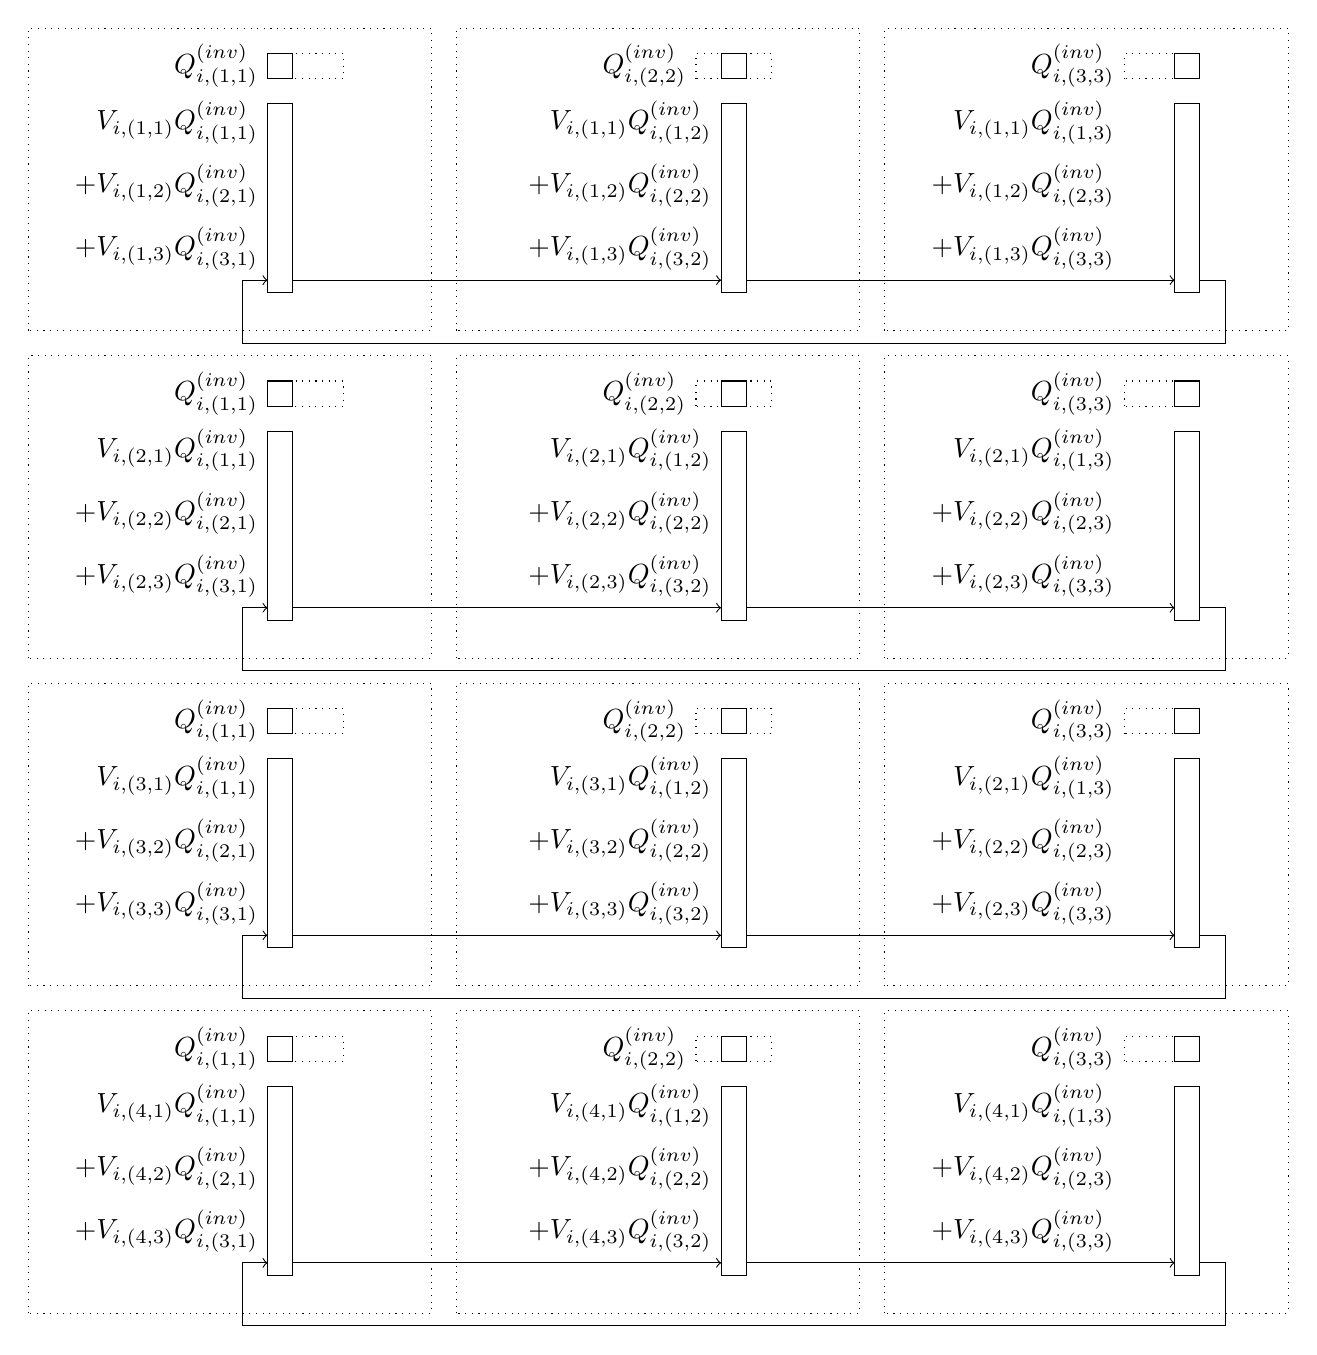
\begin{tikzpicture}[scale=16]
		% решетка процессов
		\draw [dotted] ( 0.00, 0.00 ) rectangle ( 0.32, 0.24 );
		\draw [dotted] ( 0.34, 0.00 ) rectangle ( 0.66, 0.24 );
		\draw [dotted] ( 0.68, 0.00 ) rectangle ( 1.00, 0.24 );
		\draw [dotted] ( 0.00, 0.26 ) rectangle ( 0.32, 0.50 );
		\draw [dotted] ( 0.34, 0.26 ) rectangle ( 0.66, 0.50 );
		\draw [dotted] ( 0.68, 0.26 ) rectangle ( 1.00, 0.50 );
		\draw [dotted] ( 0.00, 0.52 ) rectangle ( 0.32, 0.76 );
		\draw [dotted] ( 0.34, 0.52 ) rectangle ( 0.66, 0.76 );
		\draw [dotted] ( 0.68, 0.52 ) rectangle ( 1.00, 0.76 );
		\draw [dotted] ( 0.00, 0.78 ) rectangle ( 0.32, 1.02 );
		\draw [dotted] ( 0.34, 0.78 ) rectangle ( 0.66, 1.02 );
		\draw [dotted] ( 0.68, 0.78 ) rectangle ( 1.00, 1.02 );

		% процесс ( 1, 1 )
		\draw [dotted] ( 0.19, 0.98 ) rectangle ( 0.25, 1.00 );
		\draw ( 0.19, 0.98 ) rectangle ( 0.21, 1.00 ) node [left] at ( 0.19, 0.99 ) {$Q_{i,(1,1)}^{(inv)}$};
		\draw ( 0.19, 0.81 ) rectangle ( 0.21, 0.96 );
		\node [below left] at ( 0.19, 0.97 ) {$V_{i,(1,1)} Q_{i,(1,1)}^{(inv)}$};
		\node [below left] at ( 0.19, 0.92 ) {$+V_{i,(1,2)} Q_{i,(2,1)}^{(inv)}$};
		\node [below left] at ( 0.19, 0.87 ) {$+V_{i,(1,3)} Q_{i,(3,1)}^{(inv)}$};
		\draw [->] ( 0.21, 0.82 ) -- ( 0.55, 0.82 );

		% процесс ( 1, 2 )
		\draw [dotted] ( 0.53, 0.98 ) rectangle ( 0.59, 1.00 );
		\draw ( 0.55, 0.98 ) rectangle ( 0.57, 1.00 ) node [left] at ( 0.53, 0.99 ) {$Q_{i,(2,2)}^{(inv)}$};
		\draw ( 0.55, 0.81 ) rectangle ( 0.57, 0.96 );
		\node [below left] at ( 0.55, 0.97 ) {$V_{i,(1,1)} Q_{i,(1,2)}^{(inv)}$};
		\node [below left] at ( 0.55, 0.92 ) {$+V_{i,(1,2)} Q_{i,(2,2)}^{(inv)}$};
		\node [below left] at ( 0.55, 0.87 ) {$+V_{i,(1,3)} Q_{i,(3,2)}^{(inv)}$};
		\draw [->] ( 0.57, 0.82 ) -- ( 0.91, 0.82 );

		% процесс ( 1, 3 )
		\draw [dotted] ( 0.87, 0.98 ) rectangle ( 0.93, 1.00 );
		\draw ( 0.91, 0.98 ) rectangle ( 0.93, 1.00 ) node [left] at ( 0.87, 0.99 ) {$Q_{i,(3,3)}^{(inv)}$};
		\draw ( 0.91, 0.81 ) rectangle ( 0.93, 0.96 );
		\node [below left] at ( 0.87, 0.97 ) {$V_{i,(1,1)} Q_{i,(1,3)}^{(inv)}$};
		\node [below left] at ( 0.87, 0.92 ) {$+V_{i,(1,2)} Q_{i,(2,3)}^{(inv)}$};
		\node [below left] at ( 0.87, 0.87 ) {$+V_{i,(1,3)} Q_{i,(3,3)}^{(inv)}$};
		\draw [->] ( 0.93, 0.82 ) -- ( 0.95, 0.82 ) -- ( 0.95, 0.77 ) -- ( 0.17, 0.77 ) -- ( 0.17, 0.82 ) -- ( 0.19, 0.82 );

		% процесс ( 2, 1 )
		\draw [dotted] ( 0.19, 0.72 ) rectangle ( 0.25, 0.74 );
		\draw ( 0.19, 0.72 ) rectangle ( 0.21, 0.74 ) node [left] at ( 0.19, 0.73 ) {$Q_{i,(1,1)}^{(inv)}$};
		\draw ( 0.19, 0.55 ) rectangle ( 0.21, 0.70 );
		\node [below left] at ( 0.19, 0.71 ) {$V_{i,(2,1)} Q_{i,(1,1)}^{(inv)}$};
		\node [below left] at ( 0.19, 0.66 ) {$+V_{i,(2,2)} Q_{i,(2,1)}^{(inv)}$};
		\node [below left] at ( 0.19, 0.61 ) {$+V_{i,(2,3)} Q_{i,(3,1)}^{(inv)}$};
		\draw [->] ( 0.21, 0.56 ) -- ( 0.55, 0.56 );

		% процесс ( 2, 2 )
		\draw [dotted] ( 0.53, 0.72 ) rectangle ( 0.59, 0.74 );
		\draw ( 0.55, 0.72 ) rectangle ( 0.57, 0.74 ) node [left] at ( 0.53, 0.73 ) {$Q_{i,(2,2)}^{(inv)}$};
		\draw ( 0.55, 0.55 ) rectangle ( 0.57, 0.70 );
		\node [below left] at ( 0.55, 0.71 ) {$V_{i,(2,1)} Q_{i,(1,2)}^{(inv)}$};
		\node [below left] at ( 0.55, 0.66 ) {$+V_{i,(2,2)} Q_{i,(2,2)}^{(inv)}$};
		\node [below left] at ( 0.55, 0.61 ) {$+V_{i,(2,3)} Q_{i,(3,2)}^{(inv)}$};
		\draw [->] ( 0.57, 0.56 ) -- ( 0.91, 0.56 );

		% процесс ( 2, 3 )
		\draw [dotted] ( 0.87, 0.72 ) rectangle ( 0.93, 0.74 );
		\draw ( 0.91, 0.72 ) rectangle ( 0.93, 0.74 ) node [left] at ( 0.87, 0.73 ) {$Q_{i,(3,3)}^{(inv)}$};
		\draw ( 0.91, 0.55 ) rectangle ( 0.93, 0.70 );
		\node [below left] at ( 0.87, 0.71 ) {$V_{i,(2,1)} Q_{i,(1,3)}^{(inv)}$};
		\node [below left] at ( 0.87, 0.66 ) {$+V_{i,(2,2)} Q_{i,(2,3)}^{(inv)}$};
		\node [below left] at ( 0.87, 0.61 ) {$+V_{i,(2,3)} Q_{i,(3,3)}^{(inv)}$};
		\draw [->] ( 0.93, 0.56 ) -- ( 0.95, 0.56 ) -- ( 0.95, 0.51 ) -- ( 0.17, 0.51 ) -- ( 0.17, 0.56 ) -- ( 0.19, 0.56 );

		% процесс ( 3, 1 )
		\draw [dotted] ( 0.19, 0.46 ) rectangle ( 0.25, 0.48 );
		\draw ( 0.19, 0.46 ) rectangle ( 0.21, 0.48 ) node [left] at ( 0.19, 0.47 ) {$Q_{i,(1,1)}^{(inv)}$};
		\draw ( 0.19, 0.29 ) rectangle ( 0.21, 0.44 );
		\node [below left] at ( 0.19, 0.45 ) {$V_{i,(3,1)} Q_{i,(1,1)}^{(inv)}$};
		\node [below left] at ( 0.19, 0.40 ) {$+V_{i,(3,2)} Q_{i,(2,1)}^{(inv)}$};
		\node [below left] at ( 0.19, 0.35 ) {$+V_{i,(3,3)} Q_{i,(3,1)}^{(inv)}$};
		\draw [->] ( 0.21, 0.30 ) -- ( 0.55, 0.30 );

		% процесс ( 3, 2 )
		\draw [dotted] ( 0.53, 0.46 ) rectangle ( 0.59, 0.48 );
		\draw ( 0.55, 0.46 ) rectangle ( 0.57, 0.48 ) node [left] at ( 0.53, 0.47 ) {$Q_{i,(2,2)}^{(inv)}$};
		\draw ( 0.55, 0.29 ) rectangle ( 0.57, 0.44 );
		\node [below left] at ( 0.55, 0.45 ) {$V_{i,(3,1)} Q_{i,(1,2)}^{(inv)}$};
		\node [below left] at ( 0.55, 0.40 ) {$+V_{i,(3,2)} Q_{i,(2,2)}^{(inv)}$};
		\node [below left] at ( 0.55, 0.35 ) {$+V_{i,(3,3)} Q_{i,(3,2)}^{(inv)}$};
		\draw [->] ( 0.57, 0.30 ) -- ( 0.91, 0.30 );

		% процесс ( 3, 3 )
		\draw [dotted] ( 0.87, 0.46 ) rectangle ( 0.93, 0.48 );
		\draw ( 0.91, 0.46 ) rectangle ( 0.93, 0.48 ) node [left] at ( 0.87, 0.47 ) {$Q_{i,(3,3)}^{(inv)}$};
		\draw ( 0.91, 0.29 ) rectangle ( 0.93, 0.44 );
		\node [below left] at ( 0.87, 0.45 ) {$V_{i,(2,1)} Q_{i,(1,3)}^{(inv)}$};
		\node [below left] at ( 0.87, 0.40 ) {$+V_{i,(2,2)} Q_{i,(2,3)}^{(inv)}$};
		\node [below left] at ( 0.87, 0.35 ) {$+V_{i,(2,3)} Q_{i,(3,3)}^{(inv)}$};
		\draw [->] ( 0.93, 0.30 ) -- ( 0.95, 0.30 ) -- ( 0.95, 0.25 ) -- ( 0.17, 0.25 ) -- ( 0.17, 0.30 ) -- ( 0.19, 0.30 );

		% процесс ( 4, 1 )
		\draw [dotted] ( 0.19, 0.20 ) rectangle ( 0.25, 0.22 );
		\draw ( 0.19, 0.20 ) rectangle ( 0.21, 0.22 ) node [left] at ( 0.19, 0.21 ) {$Q_{i,(1,1)}^{(inv)}$};
		\draw ( 0.19, 0.03 ) rectangle ( 0.21, 0.18 );
		\node [below left] at ( 0.19, 0.19 ) {$V_{i,(4,1)} Q_{i,(1,1)}^{(inv)}$};
		\node [below left] at ( 0.19, 0.14 ) {$+V_{i,(4,2)} Q_{i,(2,1)}^{(inv)}$};
		\node [below left] at ( 0.19, 0.09 ) {$+V_{i,(4,3)} Q_{i,(3,1)}^{(inv)}$};
		\draw [->] ( 0.21, 0.04 ) -- ( 0.55, 0.04 );

		% процесс ( 4, 2 )
		\draw [dotted] ( 0.53, 0.20 ) rectangle ( 0.59, 0.22 );
		\draw ( 0.55, 0.20 ) rectangle ( 0.57, 0.22 ) node [left] at ( 0.53, 0.21 ) {$Q_{i,(2,2)}^{(inv)}$};
		\draw ( 0.55, 0.03 ) rectangle ( 0.57, 0.18 );
		\node [below left] at ( 0.55, 0.19 ) {$V_{i,(4,1)} Q_{i,(1,2)}^{(inv)}$};
		\node [below left] at ( 0.55, 0.14 ) {$+V_{i,(4,2)} Q_{i,(2,2)}^{(inv)}$};
		\node [below left] at ( 0.55, 0.09 ) {$+V_{i,(4,3)} Q_{i,(3,2)}^{(inv)}$};
		\draw [->] ( 0.57, 0.04 ) -- ( 0.91, 0.04 );

		% процесс ( 4, 3 )
		\draw [dotted] ( 0.87, 0.20 ) rectangle ( 0.93, 0.22 );
		\draw ( 0.91, 0.20 ) rectangle ( 0.93, 0.22 ) node [left] at ( 0.87, 0.21 ) {$Q_{i,(3,3)}^{(inv)}$};
		\draw ( 0.91, 0.03 ) rectangle ( 0.93, 0.18 );
		\node [below left] at ( 0.87, 0.19 ) {$V_{i,(4,1)} Q_{i,(1,3)}^{(inv)}$};
		\node [below left] at ( 0.87, 0.14 ) {$+V_{i,(4,2)} Q_{i,(2,3)}^{(inv)}$};
		\node [below left] at ( 0.87, 0.09 ) {$+V_{i,(4,3)} Q_{i,(3,3)}^{(inv)}$};
		\draw [->] ( 0.93, 0.04 ) -- ( 0.95, 0.04 ) -- ( 0.95, -0.01 ) -- ( 0.17, -0.01 ) -- ( 0.17, 0.04 ) -- ( 0.19, 0.04 );
	\end{tikzpicture}
	\caption{Вычисление $V_i^{(Q)}$ (вариант 2): шаг 3}
\end{figure}

\subsection{Вычисление $X_i = V_i^{(Q)} V_i^{(B)}$}

\begin{figure}
	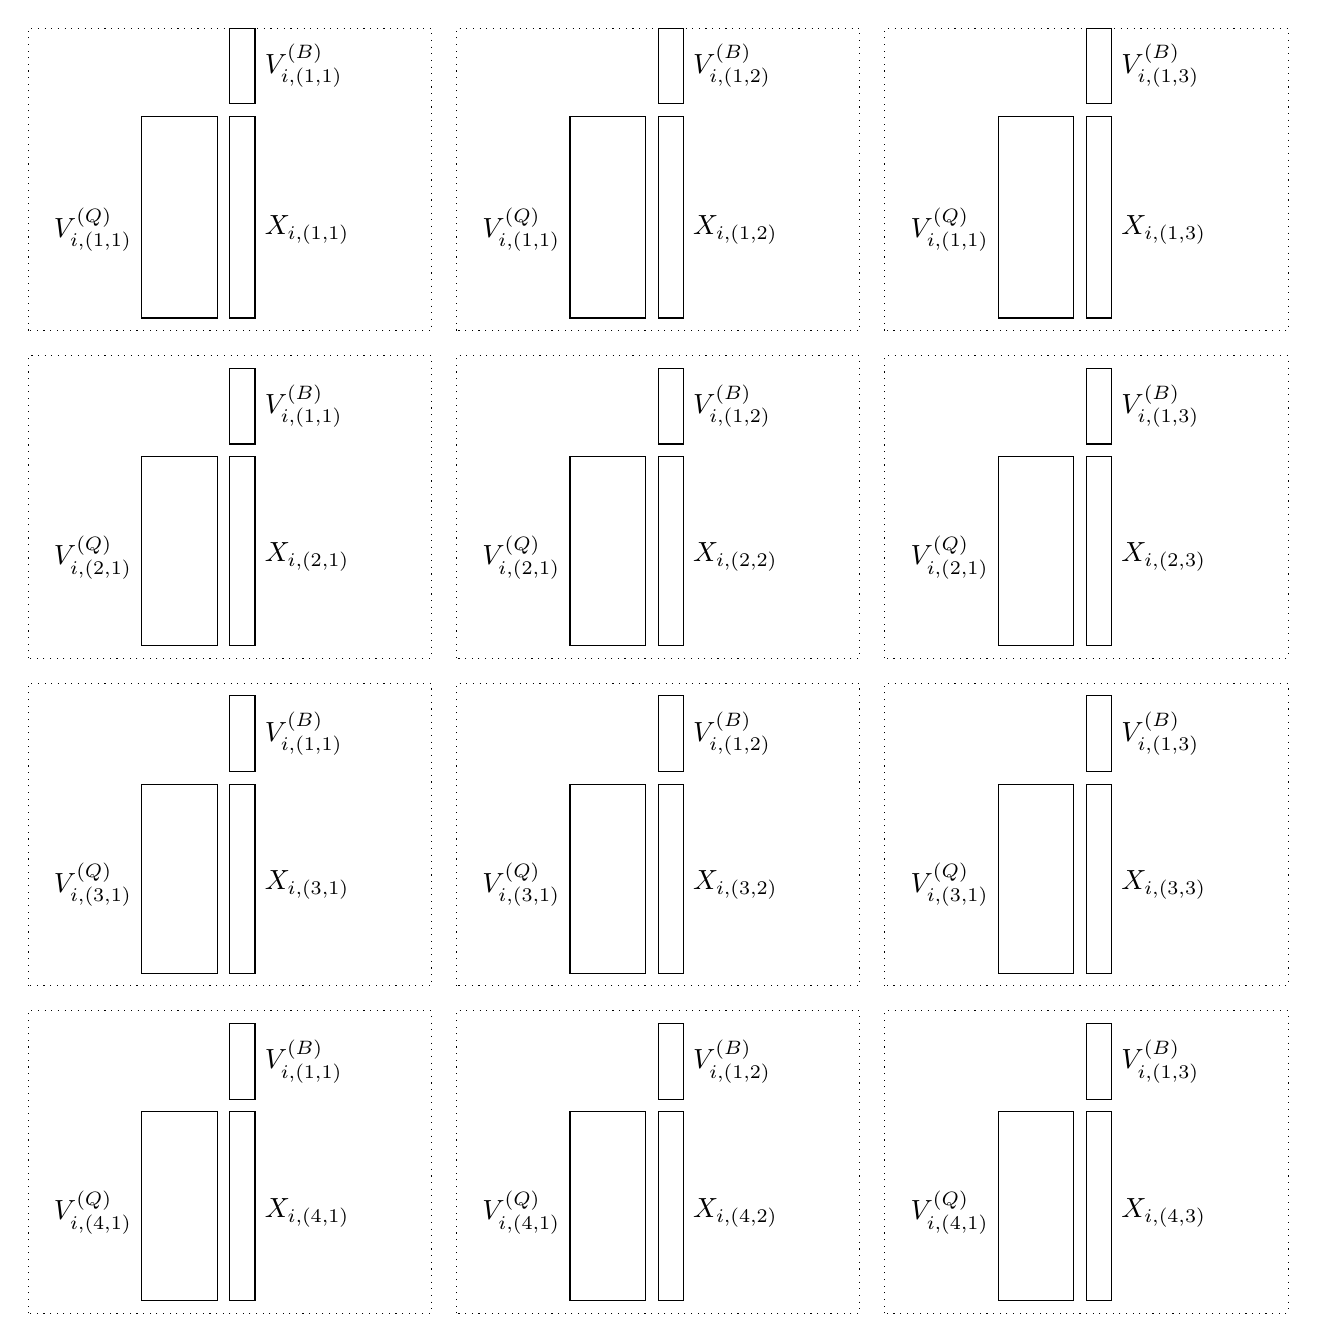
\begin{tikzpicture}[scale=16]
		% решетка процессов
		\draw [dotted] ( 0.00, 0.00 ) rectangle ( 0.32, 0.24 );
		\draw [dotted] ( 0.34, 0.00 ) rectangle ( 0.66, 0.24 );
		\draw [dotted] ( 0.68, 0.00 ) rectangle ( 1.00, 0.24 );
		\draw [dotted] ( 0.00, 0.26 ) rectangle ( 0.32, 0.50 );
		\draw [dotted] ( 0.34, 0.26 ) rectangle ( 0.66, 0.50 );
		\draw [dotted] ( 0.68, 0.26 ) rectangle ( 1.00, 0.50 );
		\draw [dotted] ( 0.00, 0.52 ) rectangle ( 0.32, 0.76 );
		\draw [dotted] ( 0.34, 0.52 ) rectangle ( 0.66, 0.76 );
		\draw [dotted] ( 0.68, 0.52 ) rectangle ( 1.00, 0.76 );
		\draw [dotted] ( 0.00, 0.78 ) rectangle ( 0.32, 1.02 );
		\draw [dotted] ( 0.34, 0.78 ) rectangle ( 0.66, 1.02 );
		\draw [dotted] ( 0.68, 0.78 ) rectangle ( 1.00, 1.02 );

		% процесс ( 1, 1 )
		\draw ( 0.09, 0.79 ) rectangle ( 0.15, 0.95 ) node [left] at ( 0.09, 0.86 ) {$V_{i,(1,1)}^{(Q)}$};
		\draw ( 0.16, 0.96 ) rectangle ( 0.18, 1.02 ) node [right] at ( 0.18, 0.99 ) {$V_{i,(1,1)}^{(B)}$};
		\draw ( 0.16, 0.79 ) rectangle ( 0.18, 0.95 ) node [right] at ( 0.18, 0.86 ) {$X_{i,(1,1)}$};

		% процесс ( 1, 2 )
		\draw ( 0.43, 0.79 ) rectangle ( 0.49, 0.95 ) node [left] at ( 0.43, 0.86 ) {$V_{i,(1,1)}^{(Q)}$};
		\draw ( 0.50, 0.96 ) rectangle ( 0.52, 1.02 ) node [right] at ( 0.52, 0.99 ) {$V_{i,(1,2)}^{(B)}$};
		\draw ( 0.50, 0.79 ) rectangle ( 0.52, 0.95 ) node [right] at ( 0.52, 0.86 ) {$X_{i,(1,2)}$};

		% процесс ( 1, 3 )
		\draw ( 0.77, 0.79 ) rectangle ( 0.83, 0.95 ) node [left] at ( 0.77, 0.86 ) {$V_{i,(1,1)}^{(Q)}$};
		\draw ( 0.84, 0.96 ) rectangle ( 0.86, 1.02 ) node [right] at ( 0.86, 0.99 ) {$V_{i,(1,3)}^{(B)}$};
		\draw ( 0.84, 0.79 ) rectangle ( 0.86, 0.95 ) node [right] at ( 0.86, 0.86 ) {$X_{i,(1,3)}$};

		% процесс ( 2, 1 )
		\draw ( 0.09, 0.53 ) rectangle ( 0.15, 0.68 ) node [left] at ( 0.09, 0.60 ) {$V_{i,(2,1)}^{(Q)}$};
		\draw ( 0.16, 0.69 ) rectangle ( 0.18, 0.75 ) node [right] at ( 0.18, 0.72 ) {$V_{i,(1,1)}^{(B)}$};
		\draw ( 0.16, 0.53 ) rectangle ( 0.18, 0.68 ) node [right] at ( 0.18, 0.60 ) {$X_{i,(2,1)}$};

		% процесс ( 2, 2 )
		\draw ( 0.43, 0.53 ) rectangle ( 0.49, 0.68 ) node [left] at ( 0.43, 0.60 ) {$V_{i,(2,1)}^{(Q)}$};
		\draw ( 0.50, 0.69 ) rectangle ( 0.52, 0.75 ) node [right] at ( 0.52, 0.72 ) {$V_{i,(1,2)}^{(B)}$};
		\draw ( 0.50, 0.53 ) rectangle ( 0.52, 0.68 ) node [right] at ( 0.52, 0.60 ) {$X_{i,(2,2)}$};

		% процесс ( 2, 3 )
		\draw ( 0.77, 0.53 ) rectangle ( 0.83, 0.68 ) node [left] at ( 0.77, 0.60 ) {$V_{i,(2,1)}^{(Q)}$};
		\draw ( 0.84, 0.69 ) rectangle ( 0.86, 0.75 ) node [right] at ( 0.86, 0.72 ) {$V_{i,(1,3)}^{(B)}$};
		\draw ( 0.84, 0.53 ) rectangle ( 0.86, 0.68 ) node [right] at ( 0.86, 0.60 ) {$X_{i,(2,3)}$};

		% процесс ( 3, 1 )
		\draw ( 0.09, 0.27 ) rectangle ( 0.15, 0.42 ) node [left] at ( 0.09, 0.34 ) {$V_{i,(3,1)}^{(Q)}$};
		\draw ( 0.16, 0.43 ) rectangle ( 0.18, 0.49 ) node [right] at ( 0.18, 0.46 ) {$V_{i,(1,1)}^{(B)}$};
		\draw ( 0.16, 0.27 ) rectangle ( 0.18, 0.42 ) node [right] at ( 0.18, 0.34 ) {$X_{i,(3,1)}$};

		% процесс ( 3, 2 )
		\draw ( 0.43, 0.27 ) rectangle ( 0.49, 0.42 ) node [left] at ( 0.43, 0.34 ) {$V_{i,(3,1)}^{(Q)}$};
		\draw ( 0.50, 0.43 ) rectangle ( 0.52, 0.49 ) node [right] at ( 0.52, 0.46 ) {$V_{i,(1,2)}^{(B)}$};
		\draw ( 0.50, 0.27 ) rectangle ( 0.52, 0.42 ) node [right] at ( 0.52, 0.34 ) {$X_{i,(3,2)}$};

		% процесс ( 3, 3 )
		\draw ( 0.77, 0.27 ) rectangle ( 0.83, 0.42 ) node [left] at ( 0.77, 0.34 ) {$V_{i,(3,1)}^{(Q)}$};
		\draw ( 0.84, 0.43 ) rectangle ( 0.86, 0.49 ) node [right] at ( 0.86, 0.46 ) {$V_{i,(1,3)}^{(B)}$};
		\draw ( 0.84, 0.27 ) rectangle ( 0.86, 0.42 ) node [right] at ( 0.86, 0.34 ) {$X_{i,(3,3)}$};

		% процесс ( 4, 1 )
		\draw ( 0.09, 0.01 ) rectangle ( 0.15, 0.16 ) node [left] at ( 0.09, 0.08 ) {$V_{i,(4,1)}^{(Q)}$};
		\draw ( 0.16, 0.17 ) rectangle ( 0.18, 0.23 ) node [right] at ( 0.18, 0.20 ) {$V_{i,(1,1)}^{(B)}$};
		\draw ( 0.16, 0.01 ) rectangle ( 0.18, 0.16 ) node [right] at ( 0.18, 0.08 ) {$X_{i,(4,1)}$};

		% процесс ( 4, 2 )
		\draw ( 0.43, 0.01 ) rectangle ( 0.49, 0.16 ) node [left] at ( 0.43, 0.08 ) {$V_{i,(4,1)}^{(Q)}$};
		\draw ( 0.50, 0.17 ) rectangle ( 0.52, 0.23 ) node [right] at ( 0.52, 0.20 ) {$V_{i,(1,2)}^{(B)}$};
		\draw ( 0.50, 0.01 ) rectangle ( 0.52, 0.16 ) node [right] at ( 0.52, 0.08 ) {$X_{i,(4,2)}$};

		% процесс ( 4, 3 )
		\draw ( 0.77, 0.01 ) rectangle ( 0.83, 0.16 ) node [left] at ( 0.77, 0.08 ) {$V_{i,(4,1)}^{(Q)}$};
		\draw ( 0.84, 0.17 ) rectangle ( 0.86, 0.23 ) node [right] at ( 0.86, 0.20 ) {$V_{i,(1,3)}^{(B)}$};
		\draw ( 0.84, 0.01 ) rectangle ( 0.86, 0.16 ) node [right] at ( 0.86, 0.08 ) {$X_{i,(4,3)}$};
	\end{tikzpicture}
	\caption{Вычисление $X_i$}
\end{figure}

\section{Заметки}

\begin{itemize}
	\item Вообще говоря теперь можно проверить нет ли среди столбцов матрицы $BW$ нулевых;
	\item что означает нулевая матрица $W_i^T S^T S W_i$?
\end{itemize}
